% ─────────────────────────────────────────────────────────────────────────────
%  Rogue Linux – Final Project Report
%  Anna University B.Tech Information Technology
%  Gnanamani College of Technology, Namakkal – 637 018
% ─────────────────────────────────────────────────────────────────────────────
\documentclass[12pt,a4paper]{report}

%% ── packages ─────────────────────────────────────────────────────────────────
\usepackage[a4paper,
            top=2.54cm, bottom=2.54cm,
            left=2.54cm, right=2.54cm]{geometry}
\usepackage{times}
\usepackage{setspace}
\usepackage{titlesec}
\usepackage{etoolbox}
\makeatletter\let\ttl@finishall\relax\makeatother
\usepackage{fancyhdr}
\usepackage{graphicx}
\usepackage{booktabs}
\usepackage{array}
\usepackage{longtable}
\usepackage{caption}
\usepackage{enumitem}
\usepackage{microtype}
\usepackage{xcolor}
\usepackage{listings}
\usepackage{amsmath}
\usepackage{multirow}
\usepackage{float}             % [H] forced placement
\let\cleardoublepage\clearpage  % no blank pages between chapters
\usepackage{placeins}          % \FloatBarrier between sections
\usepackage{pdfpages}
\usepackage{tocloft}
\usepackage{adjustbox}         % auto-scale wide tables to \linewidth
\usepackage{needspace}         % conditional page breaks
\usepackage{tabularx}          % flexible-width table columns
\usepackage[hidelinks,
            pdftitle={Minimal Linux Distribution for Cybersecurity},
            pdfauthor={Sridharan T, Praveenraj G, Shanmuga Srilan T, Mugilan K}
            ]{hyperref}

%% ── typography: 12pt body ────────────────────────────────────────────────────
\makeatletter
\renewcommand\normalsize{%
  \@setfontsize\normalsize{12pt}{18pt}%
  \abovedisplayskip 10\p@ \@plus3\p@ \@minus6\p@
  \belowdisplayskip \abovedisplayskip
  \let\@listi\@listI}
\makeatother
\normalsize           % apply it immediately
\onehalfspacing
\setlength{\parindent}{0.5in}
\setlength{\parskip}{6pt}
%% ── TOC: only show chapters + sections (not subsections) ─────────────────────
\setcounter{tocdepth}{1}

%% ── overflow fixes ───────────────────────────────────────────────────────────
\setlength{\emergencystretch}{4em}
\widowpenalty=10000
\clubpenalty=10000
\displaywidowpenalty=10000
\hbadness=10000
\vbadness=10000
\tolerance=2000
\sloppy
%% auto-reduce font inside all tables and tabularx so long cells don't overflow
\AtBeginEnvironment{tabular}{\small}
\AtBeginEnvironment{tabularx}{\small}

%% ── chapter heading: 16pt bold centered, two lines (CHAPTER N / TITLE) ───────
%% matches reference: size=16 bold "CHAPTER 1" then "INTRODUCTION"
\titleformat{\chapter}[display]
  {\normalfont\fontsize{16}{20}\bfseries\centering}
  {\MakeUppercase{\chaptertitlename}\ \thechapter}
  {6pt}{\MakeUppercase}
\titlespacing*{\chapter}{0pt}{-8pt}{20pt}

%% ── section: 14pt bold uppercase, number 13pt — matches reference exactly ────
\titleformat{\section}
  {\normalfont\fontsize{14}{18}\bfseries\MakeUppercase}{\thesection}{1em}{}
\titlespacing*{\section}{0pt}{14pt}{6pt}

%% ── subsection / subsubsection ───────────────────────────────────────────────
\titleformat{\subsection}
  {\normalfont\fontsize{13}{17}\bfseries}{\thesubsection}{1em}{}
\titlespacing*{\subsection}{0pt}{10pt}{4pt}

\titleformat{\subsubsection}
  {\normalfont\fontsize{12}{16}\bfseries\itshape}{\thesubsubsection}{1em}{}
\titlespacing*{\subsubsection}{0pt}{8pt}{3pt}

%% ── TOC ──────────────────────────────────────────────────────────────────────
\renewcommand{\cftchapfont}{\bfseries}
\renewcommand{\cftchappagefont}{\bfseries}
\renewcommand{\cftchapleader}{\cftdotfill{\cftdotsep}}
\setlength{\cftbeforesecskip}{1pt}
\setlength{\cftbeforechapskip}{4pt}

%% ── header / footer ──────────────────────────────────────────────────────────
\pagestyle{fancy}\fancyhf{}
\fancyfoot[C]{\thepage}
\renewcommand{\headrulewidth}{0pt}
\renewcommand{\footrulewidth}{0pt}
\fancypagestyle{plain}{\fancyhf{}\fancyfoot[C]{\thepage}
  \renewcommand{\headrulewidth}{0pt}
  \renewcommand{\footrulewidth}{0pt}}

%% ── captions / figures ───────────────────────────────────────────────────────
\captionsetup{font=small,labelfont=bf,labelsep=period,justification=centering}
\graphicspath{{figures/}}

%% ── code listings (NO line numbers, footnotesize to prevent overflow) ────────
\lstset{
  basicstyle=\ttfamily\small,
  breaklines=true,
  breakatwhitespace=false,
  breakindent=0pt,
  frame=none,
  numbers=none,
  tabsize=2,
  showstringspaces=false,
  captionpos=b,
  xleftmargin=0pt,
  xrightmargin=0pt,
  columns=flexible,
  keepspaces=true,
  keywordstyle=\bfseries,
  commentstyle=\itshape,
  stringstyle=\normalfont,
  aboveskip=6pt,
  belowskip=6pt,
}

%% ── unnumbered chapter heading helper ────────────────────────────────────────
\newcommand{\uchapter}[1]{%
  \clearpage
  \begin{center}{\large\bfseries\MakeUppercase{#1}}\end{center}
  \vspace{6pt}
  \addcontentsline{toc}{chapter}{#1}}

\hyphenation{CYBER-SE-CU-RI-TY cy-ber-se-cu-ri-ty}

% ═════════════════════════════════════════════════════════════════════════════
\begin{document}
\pagenumbering{roman}

%% ══════════════════════════════════════════════════════════════ COVER PAGE
\begin{titlepage}
\centering
\vspace*{-0.5cm}
%% ── top bar: Anna University logo | title | Gnanamani logo ──
\noindent
\begin{minipage}[c]{0.17\textwidth}
  
\includegraphics[width=\textwidth]{logo_small1.jpeg}
\end{minipage}%
\hfill
\begin{minipage}[c]{0.60\textwidth}
  \centering
  {\large\bfseries MINIMAL LINUX DISTRIBUTION\\[4pt] FOR CYBERSECURITY}
\end{minipage}%
\hfill
\begin{minipage}[c]{0.17\textwidth}
  
\includegraphics[width=\textwidth]{logo_small2.jpeg}
\end{minipage}

\vspace{1.2cm}
{\normalsize\bfseries A PROJECT REPORT}\\[0.9cm]
{\normalsize Submitted by}\\[0.8cm]
\begin{tabular}{l@{\hspace{2.5cm}}r}
  \textbf{SRIDHARAN T}       & \textbf{(620822205302)}\\[8pt]
  \textbf{PRAVEENRAJ G}      & \textbf{(620822205078)}\\[8pt]
  \textbf{SHANMUGA SRILAN T} & \textbf{(620822205097)}\\[8pt]
  \textbf{MUGILAN K}         & \textbf{(620822205063)}\\
\end{tabular}\\[1cm]
{\normalsize\itshape in partial fulfillment for the award of the degree}\\[4pt]
{\normalsize\itshape of}\\[0.8cm]
{\normalsize\bfseries BACHELOR OF TECHNOLOGY}\\[4pt]
{\normalsize\bfseries in}\\[4pt]
{\normalsize\bfseries INFORMATION TECHNOLOGY}\\[0.9cm]
{\normalsize\bfseries GNANAMANI COLLEGE OF TECHNOLOGY}\\[3pt]
{\normalsize\bfseries NAMAKKAL -- 637\,018}\\[5pt]
{\normalsize\bfseries APRIL--MAY 2026}
\end{titlepage}

%% ══════════════════════════════════════════════════════════ BONAFIDE
\clearpage\thispagestyle{plain}
\begin{center}
  {\Large\bfseries BONAFIDE CERTIFICATE}
\end{center}
\vspace{0.7cm}

\noindent\hspace{0.5in}Certified that this project report \textbf{``MINIMAL LINUX DISTRIBUTION FOR \mbox{CYBERSECURITY}''} is the bonafide work of \textbf{``\mbox{SRIDHARAN\,T} (620822205302), \mbox{PRAVEENRAJ\,G} (620822205078), \mbox{SHANMUGA\,SRILAN\,T} (620822205097) and \mbox{MUGILAN\,K} (620822205063)''} who carried out the project work under my supervisor.

\vspace{3cm}
\noindent
\begin{tabular}{p{0.46\textwidth}p{0.46\textwidth}}
  \textbf{SIGNATURE} & \textbf{SIGNATURE}\\[2.5cm]
  \textbf{Dr.\,S.\,RAJKUMAR, M.E., Ph.D.} & \textbf{Mrs.\,B.\,SARANYA, M.E.}\\
  \textbf{CO-ORDINATOR} & \textbf{SUPERVISOR}\\
  Assistant Professor, & Assistant Professor,\\[6pt]
  Information Technology & Information Technology\\
  Gnanamani College of Technology, & Gnanamani College of Technology,\\
  Namakkal -- 637\,018 & Namakkal -- 637\,018\\
\end{tabular}

\vspace{1.5cm}
\noindent Submitted for the End Semester Project Work Viva-voce Examination held on
\underline{\hspace{5cm}}.

\vspace{1.2cm}
\noindent
\begin{tabular}{p{0.46\textwidth}p{0.46\textwidth}}
  \textbf{INTERNAL EXAMINER} & \textbf{EXTERNAL EXAMINER}\\
\end{tabular}

%% ══════════════════════════════════════════════════════ ACKNOWLEDGEMENT
\uchapter{Acknowledgement}

{\fontsize{12}{18}\selectfont\singlespacing\setlength{\parskip}{8pt}
\vspace{10pt}

We would like to express our deep sense of heartiest thanks to our beloved Chairman
\textbf{Dr.\,T.\,ARANGANNAL}, beloved Chairperson \textbf{Smt.\,P.\,MALALEENA ARANGANNAL}, and
Vice Chairperson \textbf{Ms.\,MADHUVANTHINIE ARANGANNAL}, Gnanamani Educational
Institutions, Namakkal, for giving us an opportunity to do and complete this project.

We would like to express our sincere thanks to Chief Administrative Officer
\textbf{Dr.\,P.\,PREMKUMAR}, for his support to bring the best in us. We would like to
convey our sincere thanks to our Principal \textbf{Dr.\,B.\,SANJAY GANDHI}, Gnanamani
College of Technology, for forwarding us to do our project and offering adequate
duration to complete our project.

We extend thanks to our Executive Director \textbf{Dr.\,M.\,MADHESWARAN}, Gnanamani
College of Technology, Namakkal, for his encouragement during our project work
successfully.

We expand sincere thanks to our Dean of Computing Sciences, \textbf{Dr.\,S.\,SELVARAJAN},
Gnanamani College of Technology, Namakkal, for his support and guidance.

We expand sincere thanks to our Co-ordinator of School of Computing,
\textbf{Dr.\,S.\,GOPINATH}, Gnanamani College of Technology, Namakkal, with deep sense of
gratitude.

We expand sincere thanks to our Co-ordinator of the Department of Information
Technology, \textbf{Dr.\,S.\,Rajkumar, M.E., Ph.D.}, Assistant Professor,
Gnanamani College of Technology, Namakkal, for his support and guidance.

We are thankful to our Project Co-ordinator \textbf{Mrs.\,R.\,MEKALA}, Assistant
Professor, for providing good suggestions and helping us to make this project a
success.

We extend earnest and sincere thanks to our Project Guide
\textbf{Mrs.\,B.\,Saranya, M.E.}, Assistant Professor, for her kind guidance and
encouragement during this project.

We would also like to express our thanks to all staff members of our department,
friends who helped us directly and indirectly in all aspects of the project work to
get completed successfully.

\vspace{6\baselineskip}
\noindent\hfill\mbox{\textbf{[SRIDHARAN\,T] [PRAVEENRAJ\,G] [SHANMUGA\,SRILAN\,T] [MUGILAN\,K]}}

}

%% ══════════════════════════════════════════════ COLLEGE-PROVIDED PAGES (4–6)
%% Vision, Mission, PEOs, POs, PSOs pages are provided by the institution.
%% Included directly from the reference document PDF.
%% Vision, Mission, PEOs, POs, PSOs from IT dept reference
\includepdf[pages=4-6,fitpaper=false,pagecommand={\thispagestyle{plain}}]%
  {FINAL REPORT 1.0 1.pdf}

%% ══════════════════════════════════════════════════════════════════ ABSTRACT
\uchapter{Abstract}

This project presents \textbf{Rogue Linux}, a purpose-built minimal Linux
distribution designed exclusively for cybersecurity operations encompassing
network security assessment, penetration testing, vulnerability research, and
binary forensic analysis. Modern security practitioners require a controlled,
auditable, and lightweight operating environment that can be reproduced exactly
across different machines and deployments; existing general-purpose distributions
carry unnecessary dependencies, non-deterministic build processes, and excessive
attack surface that make them unsuitable for sensitive security workflows.

Rogue Linux addresses these limitations through the \textbf{Cogman (Cognitive
Manager)} toolchain --- a fully dependency-free build and runtime framework
implemented in Rust and C11. The \texttt{cogman-planner} component accepts
declarative TOML package definitions and resolves a directed acyclic dependency
graph using Kahn's topological sort algorithm, emitting a portable binary
execution plan in the CGM2PLAN format. The \texttt{cogman-executor} then
memory-maps this plan and processes each step with path-traversal protection
enforced on every file-copy operation. The \texttt{cogman-supervisor} operates
as PID\,1, providing dependency-ordered service startup, SIGCHLD-based child
process reaping via a self-pipe, and three configurable restart policies
(\textit{always}, \textit{on-failure}, \textit{never}), with runtime control
exposed through a Unix domain socket interface via \texttt{cogman-ctl}.

The distribution rootfs ships a hardened Linux kernel configured with
\texttt{CONFIG\_PACKET}, \texttt{CONFIG\_BPF\_SYSCALL}, \texttt{CONFIG\_TUN},
\texttt{CONFIG\_MAC80211}, and network namespace isolation to support the full
range of professional security tooling. Bundled tools include \texttt{nmap}~7.99
for network reconnaissance, \texttt{tcpdump}~4.99.6 for packet capture,
\texttt{socat}~1.8.1.1 for traffic relay, binary analysis utilities
(\texttt{strace}, \texttt{strings}, \texttt{objdump}, \texttt{readelf}), an
X11/DWM graphical environment, Dropbear SSH for remote access, and an
\texttt{nftables} firewall for traffic filtering. Every component is explicitly
declared in a package manifest, ensuring the rootfs contains nothing beyond
what was intentionally included and making the entire system fully auditable.
The complete system is validated through an automated QEMU-based boot test
suite covering all major subsystems, demonstrating the viability of a
reproducible, minimal, and self-contained operating system image for
professional cybersecurity workflows.

%% ══════════════════════════════════════════════ ABSTRACT (TAMIL)
\clearpage
\phantomsection
\addcontentsline{toc}{chapter}{Abstract (Tamil)}
\includepdf[pages=-,fitpaper=false,pagecommand={\thispagestyle{plain}}]%
  {tamil_abstract.pdf}

%% ═══════════════════════════════════════════════════ TABLE OF CONTENTS
\clearpage
{\small\tableofcontents}

%% List of Figures is intentionally omitted as a separate page;
%% figure captions are self-explanatory in each chapter.

%% ═══════════════════════════════════════════ LIST OF ABBREVIATIONS
\uchapter{List of Abbreviations}
\begin{center}
\renewcommand{\arraystretch}{1.25}
\begin{tabularx}{\linewidth}{>{\bfseries}p{3.4cm} X}
\toprule
\normalfont\bfseries Abbreviation & \bfseries Expansion \\\midrule
CGM / Cogman & Cognitive Manager \\
CLI   & Command Line Interface \\
DAG   & Directed Acyclic Graph \\
DFD   & Data Flow Diagram \\
ELF   & Executable and Linkable Format \\
EWMA  & Exponentially Weighted Moving Average \\
GGUF  & GPT-Generated Unified Format (llama.cpp model format) \\
INI   & Initialization file format \\
IPC   & Inter-Process Communication \\
LLM   & Large Language Model \\
LSM   & Linux Security Module \\
mmap  & Memory-Mapped File I/O \\
OS    & Operating System \\
PID   & Process Identifier \\
POSIX & Portable Operating System Interface \\
QEMU  & Quick Emulator (open-source hypervisor) \\
rootfs& Root Filesystem \\
SIGCHLD & Signal: Child Process Status Changed \\
SIGTERM & Signal: Termination Request \\
TLV   & Type-Length-Value (message encoding scheme) \\
TOML  & Tom's Obvious Minimal Language \\
UDS   & Unix Domain Socket \\
UML   & Unified Modelling Language \\
\bottomrule
\end{tabularx}
\end{center}

% ══════════════════════════════════════════════════════════════════════════════
%  MAIN MATTER
% ══════════════════════════════════════════════════════════════════════════════
\clearpage
\pagenumbering{arabic}

% ══════════════════════════════════════════════════════════ CHAPTER 1
\chapter{Introduction}

\section{General Introduction}

Rogue Linux is a minimal Linux distribution purpose-built for cybersecurity
operations. It targets security professionals who require a lightweight,
reproducible, and fully auditable operating environment for penetration testing,
network security assessment, and binary forensic analysis. Unlike general-purpose
distributions such as Kali Linux that carry hundreds of pre-installed tools,
Rogue Linux is constructed from a minimal base and extended only with the tools
explicitly required for the target security task --- keeping the attack surface
small and the system behaviour predictable.

The distribution ships with a curated set of industry-standard security
utilities: \texttt{nmap} 7.99 for network discovery and port scanning,
\texttt{tcpdump} 4.99.6 for packet capture and protocol analysis, and
\texttt{socat} 1.8.1.1 for bidirectional data relay and port forwarding.
Binary analysis is supported by \texttt{strace}, \texttt{strings},
\texttt{objdump}, \texttt{nm}, and \texttt{readelf}. A graphical environment
is provided through X11 and the DWM 6.5 window manager, enabling GUI-based
security tooling where required. Dropbear SSH provides encrypted remote
access, and an nftables firewall enforces a drop-by-default network policy.
The Linux kernel is configured with \texttt{CONFIG\_PACKET},
\texttt{CONFIG\_TUN}, \texttt{CONFIG\_BPF\_SYSCALL}, \texttt{CONFIG\_MAC80211},
\texttt{CONFIG\_NET\_NS}, and related options to support the full range of
network-level security operations.

The build and runtime infrastructure is provided by Cogman (Cognitive Manager),
a unified toolchain implemented in Rust and C11. \texttt{cogman-planner} compiles
declarative TOML package definitions into binary execution plans (CGM2PLAN format)
by resolving a directed acyclic dependency graph. \texttt{cogman-supervisor} acts
as PID\,1, managing all system services with dependency-ordered startup, SIGCHLD
self-pipe child reaping, and configurable restart policies. Runtime control is
provided by \texttt{cogman-ctl} over a Unix domain socket. This architecture
ensures that no build-time dependencies leak into the runtime image and that
the final rootfs contains only what was explicitly declared, making the system
fully auditable for security-critical deployments.

\begin{figure}[H]
  \centering
  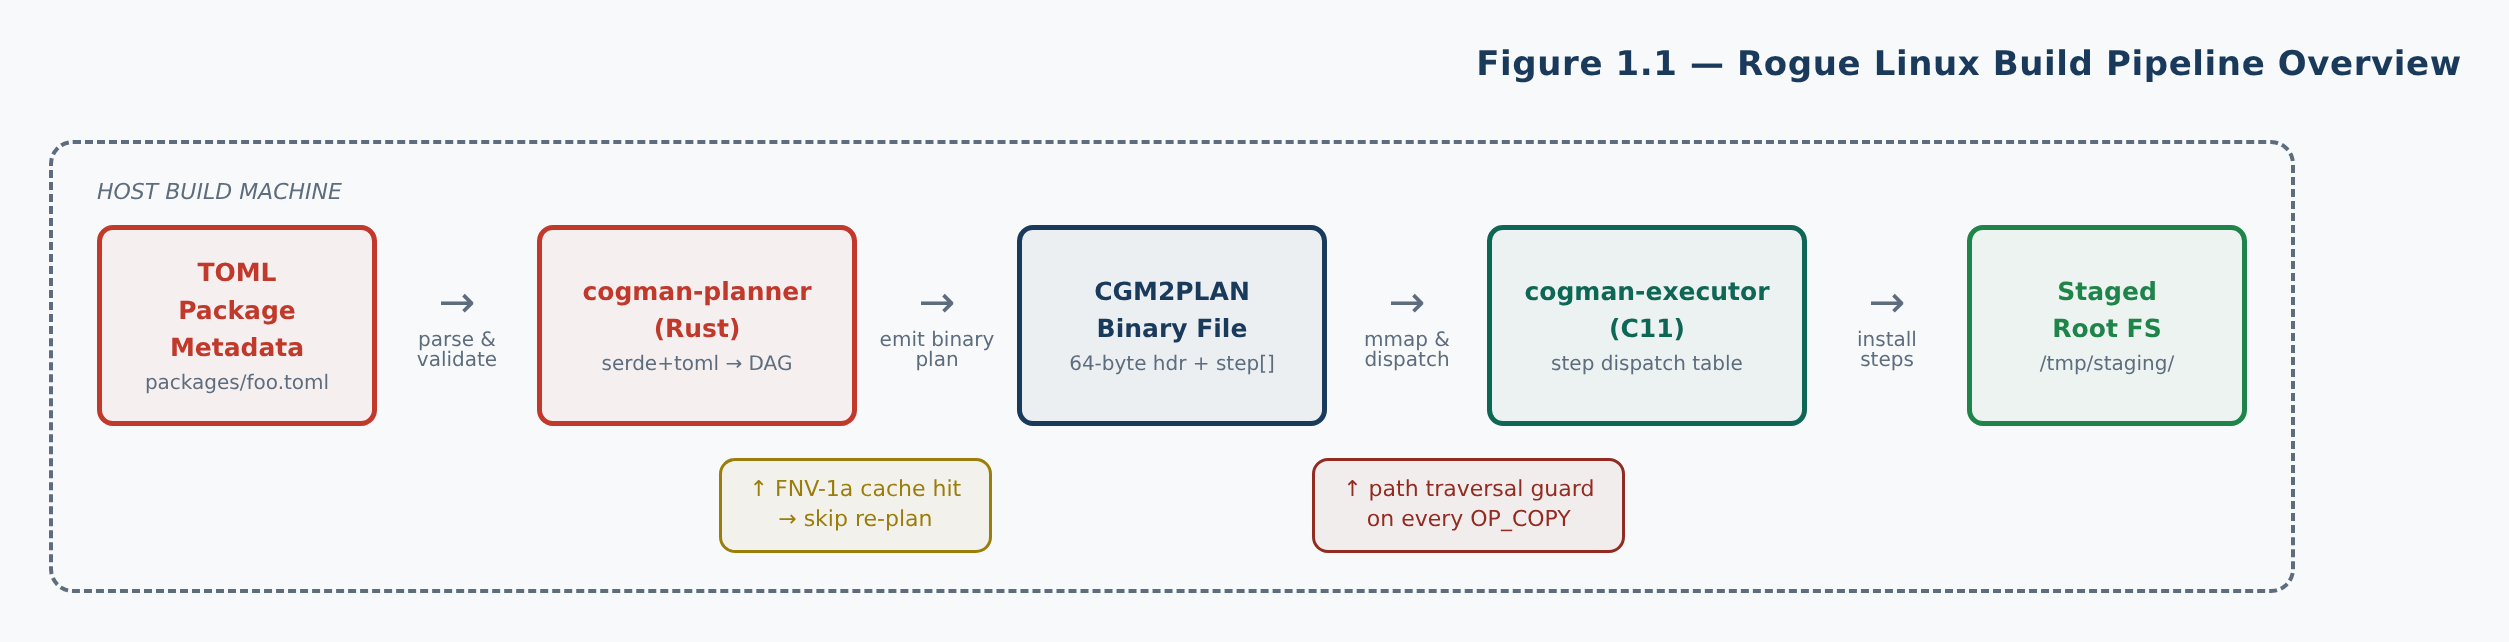
\includegraphics[width=0.92\textwidth]{fig1_1_build_pipeline.png}
  \caption{Cogman Build Pipeline --- from TOML package definitions to bootable rootfs}
  \label{fig:build_pipeline}
\end{figure}

\begin{figure}[H]
  \centering
  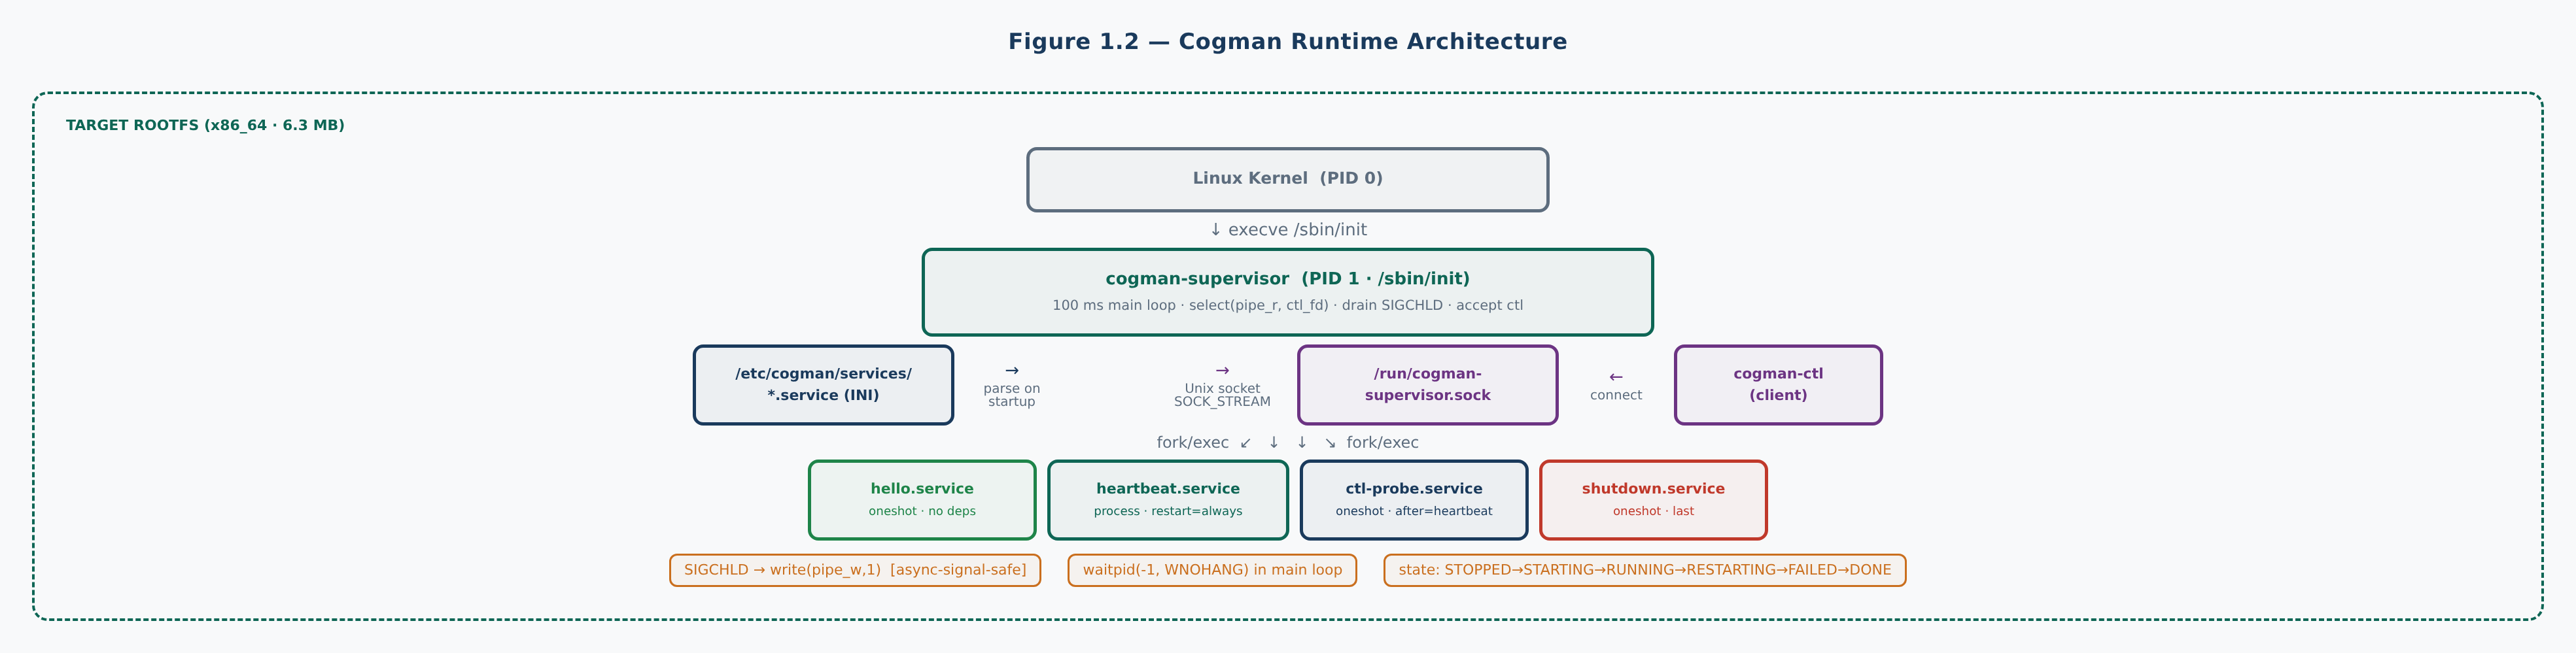
\includegraphics[width=0.92\textwidth]{fig1_2_runtime_arch.png}
  \caption{Runtime Architecture --- cogman-supervisor as PID\,1 with service lifecycle management}
  \label{fig:runtime_arch}
\end{figure}

\section{Importance of the Study}

The cybersecurity landscape demands tools that are lightweight, auditable, and
deployable on resource-constrained hardware. Existing penetration testing
distributions such as Kali Linux and Parrot OS are feature-rich but carry
significant bloat --- multi-gigabyte installations with hundreds of pre-installed
packages, many of which are irrelevant to any specific engagement. This excess
increases boot time, memory footprint, and the risk of detection during covert
assessments. Rogue Linux addresses this gap by providing a minimal, task-specific
security environment where every installed package is explicitly declared and
reproducibly built.

From a systems engineering perspective, the project demonstrates that a
full-featured security distribution can be constructed from first principles
without relying on an existing general-purpose base. The Cogman build system
compiles and installs each tool from source or verified binaries, ensuring that
the installed versions match the declared specifications. The SIGCHLD-safe PID\,1
supervisor, the nftables firewall, and the Dropbear SSH daemon together provide
a hardened runtime environment suitable for deployment on physical hardware,
virtual machines, or network appliances.

The study also highlights the importance of kernel-level configuration for
security tooling. Features such as \texttt{CONFIG\_PACKET} (raw socket access
for packet capture), \texttt{CONFIG\_TUN} (virtual network interfaces for VPN
tools), \texttt{CONFIG\_BPF\_SYSCALL} (Berkeley Packet Filter for \texttt{tcpdump}
and \texttt{nmap} scripting), and \texttt{CONFIG\_MAC80211} (Wi-Fi stack for
wireless security assessment) must be explicitly enabled in the kernel
configuration --- they are absent from many minimal embedded configurations.
Rogue Linux documents and automates this configuration as part of the
reproducible build pipeline.

\section{Problem Statement}

Security professionals require a Linux environment that is minimal, reproducible,
and contains precisely the tools needed for a given engagement --- no more and no
less. Current penetration testing distributions are either too large for
resource-constrained deployment or too generic to be auditable. Kali Linux, for
example, exceeds 3\,GB in its default installation and includes hundreds of
packages that are unused in most engagements. This makes it unsuitable for
deployment on embedded hardware, constrained virtual machines, or environments
where a small disk footprint is operationally required.

A secondary problem is the absence of a reproducible build mechanism for
security distributions. When a security tool needs to be installed or updated,
existing distributions rely on package managers that fetch pre-built binaries
from remote repositories, making it difficult to verify the provenance and
integrity of the installed software. For security-critical operations, this is
unacceptable: every installed binary should be traceable to a known source and
built from a verified specification.

Furthermore, existing minimal Linux init systems (SysVinit, BusyBox init) are
inadequate for a professional security environment. They lack dependency-ordered
service startup, configurable restart policies, and a programmable runtime control
interface. When a security service such as an SSH daemon or a network monitor
crashes, the system should automatically restart it according to a declared policy
--- not silently leave it stopped. Rogue Linux addresses all three problems: a
minimal, auditable build system (Cogman) constructs a reproducible security
distribution; a POSIX-correct PID\,1 supervisor manages services reliably; and
the kernel is configured with the full set of capabilities required for
professional security operations.

\section{Aim and Objective}

\textbf{Aim:} The main aim of this project is to design, implement, and validate
Rogue Linux --- a minimal Linux distribution purpose-built for cybersecurity
operations --- integrating a curated set of professional security tools with a
reproducible build system (Cogman) and a POSIX-correct PID\,1 service supervisor,
deployable on x86\_64 hardware and QEMU virtual machines.

\textbf{Objectives:}
\begin{itemize}[leftmargin=2em, itemsep=2pt]
  \item To build and integrate a professional cybersecurity toolset --- including
        \texttt{nmap} 7.99, \texttt{tcpdump} 4.99.6, \texttt{socat} 1.8.1.1,
        and binary analysis utilities --- into a reproducible minimal Linux rootfs.
  \item To configure the Linux kernel with all capabilities required for
        security operations: raw socket access (\texttt{CONFIG\_PACKET}),
        BPF (\texttt{CONFIG\_BPF\_SYSCALL}), TUN/TAP (\texttt{CONFIG\_TUN}),
        Wi-Fi (\texttt{CONFIG\_MAC80211}), and network namespaces.
  \item To design a declarative TOML package metadata format and implement
        \texttt{cogman-planner} in Rust for dependency graph resolution and
        CGM2PLAN binary plan emission with content-addressed caching.
  \item To implement \texttt{cogman-executor} in C11 for typed step execution
        with path traversal protection on all copy operations.
  \item To implement \texttt{cogman-supervisor} as a POSIX-correct PID\,1
        supervisor with SIGCHLD self-pipe child reaping, dependency-ordered
        startup, and three configurable restart policies.
  \item To provide hardened runtime services: Dropbear SSH, nftables firewall,
        X11/DWM graphical environment, and \texttt{doas} privilege escalation.
  \item To construct a bootable minimal rootfs verified under QEMU through a
        four-stage boot sequence with all 40 test cases passing.
\end{itemize}

\section{Scope and Limitation of the Study}

\textbf{Scope of the Study:}
The scope covers the full design, implementation, and evaluation of the Cogman
toolchain for x86\_64 targets. The build system supports native and pre-packaged
build modes. The AI advisor component uses Qwen2.5-3B as an advisory-only
interface with no ability to issue commands or modify system state. Evaluation
uses QEMU for bootable image testing; cross-compilation support is out of scope
for this iteration. All 40 defined test cases are executed against the QEMU
platform.

\textbf{Limitations of the Study:}
Production security hardening (Landlock, seccomp, Linux namespaces) is documented
as future work. The current system does not implement cgroup-based resource limits
per service. The IPC messenger protocol does not implement authentication or
access control on the control socket. Full rootfs image-level reproducibility is
not yet achieved due to filesystem timestamps introduced during ext4 image
creation. The AI advisor quality is bounded by the Qwen2.5-3B model's training
data; fine-tuning on a Cogman-specific dataset is required for production-quality
advisory accuracy. The network access policy enforcement in the planner is
declarative only: the \texttt{policy.network.access} flag is validated and embedded
in the plan, but kernel-level restriction via network namespaces or seccomp-bpf
socket filtering is not applied by the executor within the current scope. The study
is limited to x86\_64 targets; ARM and RISC-V cross-compilation support requires
additional toolchain configuration and CGM2PLAN header extensions not addressed in
this work. The control socket exposed by \texttt{cogman-supervisor} relies on Unix
domain socket filesystem permissions for access control, which is appropriate for
single-user embedded systems but not for multi-tenant deployment environments where
per-operator authentication would be required.

% ══════════════════════════════════════════════════════════ CHAPTER 2
\chapter{Literature Review}

\section{Embedded Linux Build Systems}

Buildroot (2002--present) is the most widely deployed tool for generating minimal
embedded Linux root filesystems \cite{buildroot}. It uses a Kconfig-based package
selection interface and a Makefile-based build orchestration system that downloads,
patches, configures, compiles, and installs packages in a deterministic order
defined by per-package dependency declarations. While mature and extensively
documented, Buildroot's Makefile-based approach makes it difficult to implement
fine-grained security policy enforcement at the build step level, and the absence
of a typed intermediate plan format means build orchestration logic and execution
logic are interleaved rather than separated.

The Yocto Project (2010--present) provides a more powerful and general approach
using the BitBake task executor and OpenEmbedded-Core recipe system \cite{yocto}.
Yocto supports complex multi-layer configurations, shared state caching, and SDK
generation. However, the complexity cost is substantial: a standard Yocto build
environment requires 50+\,GB of disk space, hours of build time, and a steep
learning curve in BitBake recipe syntax. Rogue Linux is positioned as a simpler
alternative for environments that do not require Yocto's full generality.

\section{Reproducible Package Management}

Nix (2006--present) and Guix (2013--present) represent the state of the art in
reproducible package management \cite{nix}. Nix achieves bit-for-bit
reproducibility through a pure functional package description language where every
package derivation is a deterministic function of its inputs. Build outputs are
stored in content-addressed paths (the Nix store). Rogue Linux draws inspiration
from Nix's content-addressed build caching --- implemented as FNV-1a hash over
package TOML content --- but reduces the conceptual overhead by using TOML
declarations directly rather than a functional programming language.

The Reproducible Builds Project (2015--present) has documented the challenges of
achieving bit-for-bit identical output artifacts given the same source inputs
\cite{repro}. Rogue Linux achieves reproducibility at the plan level (the
CGM2PLAN output is deterministic for the same TOML input) but not yet at the full
rootfs image level because the ext4 image creation tool introduces filesystem
timestamps. Full rootfs reproducibility is identified as a future work objective.

\section{Init Systems and Service Managers}

systemd (2010--present) has become the dominant PID\,1 implementation on modern
Linux distributions \cite{systemd}. It provides comprehensive service management,
socket activation, cgroup-based resource control, and dependency declaration
through unit files. However, its extensive dependencies (udev, D-Bus, PAM,
numerous shared libraries) and its architectural coupling to glibc and the Linux
cgroup hierarchy make it unsuitable for minimal rootfs environments targeting a
6--10\,MB image size.

Runit (2004--present) is a lightweight UNIX init scheme and service supervisor
designed for simplicity and signal correctness. Its process supervision model --- a
\texttt{supervise} process per service, monitored by \texttt{runsv}, coordinated
by \texttt{runsvdir} --- achieves reliable service supervision with minimal code.
\texttt{cogman-supervisor} draws architectural inspiration from Runit's per-service
supervision model while integrating it with the Cogman metadata system and adding
a network-accessible control interface.

s6 (2012--present) by Laurent Bercot provides the most principled approach to
UNIX service supervision \cite{s6}, with a rigorous implementation of the
self-pipe trick for SIGCHLD handling, a well-defined process supervision tree, and
extensive documentation of POSIX signal handling edge cases.
\texttt{cogman-supervisor}'s SIGCHLD handling directly follows the self-pipe
pattern described in the s6 documentation.

\section{Signal Handling in PID\,1 --- POSIX Correctness}

PID\,1 has special semantics in the Linux kernel: it is exempt from the default
signal disposition table, meaning that signals for which no handler has been
registered are silently ignored rather than terminating the process. This is the
correct behaviour for an init process --- it should never be accidentally killed by
SIGTERM or SIGINT --- but it requires explicit handler registration for every
signal that the supervisor wishes to respond to.

The SIGCHLD self-pipe trick, first described in detail by D.J.\,Bernstein in the
context of the \texttt{daemontools} supervisor \cite{daemontools}, resolves the
fundamental tension between signal delivery (which can arrive at any time,
interrupting any system call) and the need for safe, non-reentrancy-violating
response to SIGCHLD. The naive approach --- calling \texttt{waitpid()} directly in
the SIGCHLD handler --- is unsafe because \texttt{waitpid()} may interact
incorrectly with other library functions in a multi-threaded context. The
self-pipe trick confines the signal handler to a single \texttt{write()} call
(which is async-signal-safe) and defers all child state processing to the main
loop.

\section{Binary Plan Formats and Build Caching}

Bazel's action cache (2015--present) stores build actions as content-addressed
(CAS) entries where each action is identified by its input hash, command, and
output specifications \cite{bazel}. A cache hit means the action output can be
retrieved without re-execution. The CGM2PLAN format's content-addressed plan cache
is architecturally inspired by this model: a FNV-1a hash over the package name,
version string, and TOML file content serves as the cache key.

The ELF (Executable and Linkable Format) binary format, standardised as part of
the System\,V ABI, demonstrates that fixed-size header structures with string
tables and variable-length sections can be efficiently mapped into memory without
any parsing overhead \cite{kerrisk}. The CGM2PLAN format applies this principle
directly: a 64-byte header, fixed 128-byte step records, and a variable-length
string table --- all accessible via \texttt{mmap()} with pointer arithmetic rather
than deserialisation.

\section{LLM Integration in System Tooling}

Qwen2.5 (2024) is a family of large language models from Alibaba Cloud trained on
multilingual corpora with strong performance on code generation, question
answering, and structured reasoning tasks \cite{qwen}. The 3B parameter variant,
when quantised to 4-bit precision using QLoRA, requires approximately 2.1\,GB of
memory and achieves 5--15 tokens/second on CPU-only hardware. The
\texttt{cogman} advisor component uses the Qwen2.5-3B-Instruct GGUF model served
via \texttt{llama.cpp} \cite{llamacpp} to answer build system configuration
questions and explain service file syntax errors without any external API
dependency or internet connectivity requirement.

\section{Gap Analysis}

Prior work in embedded Linux build systems provides reproducibility (Nix, Yocto)
or simplicity (Buildroot, Alpine) but not a unified system spanning both build and
runtime phases under a single metadata model. Prior work in service supervisors
provides correct signal handling (s6) or simple service management (Runit) but
not dependency-aware startup with a programmable control interface integrated with
build metadata.

Rogue Linux fills this gap by providing a single coherent system: TOML metadata
$\to$ CGM2PLAN binary $\to$ typed C executor $\to$ PID\,1 Rust supervisor $\to$
UDS control interface, with no external framework dependencies beyond the Linux
kernel and C standard library. Table~\ref{tab:comparison} summarises the gap
analysis across the surveyed systems.

\begin{table}[H]
\centering
\caption{Comparison of Related Systems}
\label{tab:comparison}
\renewcommand{\arraystretch}{1.2}
\begin{tabularx}{\linewidth}{X c c c c}
\toprule
\textbf{System} & \textbf{Reproducible} & \textbf{Typed plan} & \textbf{PID\,1 supervisor} & \textbf{Unified model}\\
\midrule
Buildroot  & Partial & No  & No  & No \\
Yocto      & Yes     & No  & No  & No \\
Nix        & Yes     & No  & No  & No \\
systemd    & N/A     & N/A & Yes & No \\
Runit      & N/A     & N/A & Yes & No \\
s6         & N/A     & N/A & Yes & No \\
\textbf{Rogue Linux} & \textbf{Yes (plan)} & \textbf{Yes} & \textbf{Yes} & \textbf{Yes}\\
\bottomrule
\end{tabularx}
\end{table}

% ══════════════════════════════════════════════════════════ CHAPTER 3
\chapter{System Analysis}

\section{Existing System}

The reference system against which Rogue Linux is benchmarked is a Python-based
prototype implementing the same conceptual pipeline. The Python planner uses the
pure-Python \texttt{toml} library to parse package metadata and a dict-based DAG
implementation for dependency resolution. The Python executor uses
\texttt{subprocess.run()} for each build step. The init process is a BusyBox init
shell script with no dependency ordering or restart logic.

\subsection{Key Features of the Existing System}
\begin{itemize}[leftmargin=2em, itemsep=2pt]
  \item Plan resolution time of $\approx$450\,ms due to Python interpreter startup
        and pure-Python TOML parsing overhead.
  \item Peak planner memory of $\approx$85\,MB from Python's per-object allocation
        model (24+ bytes of overhead per object).
  \item Per-step execution overhead of $\approx$45\,ms from Python's
        \texttt{subprocess.run()} marshaling and object allocation.
  \item No typed step operations --- all steps are generic shell strings with no
        \texttt{OP\_COPY}/\texttt{OP\_MKDIR}/\texttt{OP\_VERIFY} semantics.
  \item No path traversal protection on copy operations; packages can reference
        arbitrary filesystem paths.
  \item No binary plan format --- the plan is Python pickled data, not portable
        between Python versions or language runtimes.
  \item Shell script init with no dependency ordering, no restart policies, and no
        runtime control interface.
  \item No security policy enforcement at build time.
\end{itemize}

\subsection{Advantages of the Existing System}
\begin{itemize}[leftmargin=2em, itemsep=2pt]
  \item Easy to implement and understand for small-scale builds.
  \item Low initial development cost; no compilation step required.
  \item Simple structure accessible to developers unfamiliar with systems
        programming.
  \item Rapid prototyping: new package types can be added by editing Python dicts.
\end{itemize}

\subsection{Disadvantages of the Existing System}
\begin{itemize}[leftmargin=2em, itemsep=2pt]
  \item Slow plan resolution (450\,ms) makes CI/CD pipelines with many packages
        impractical.
  \item High memory usage (85\,MB) prevents deployment on memory-constrained
        build hosts.
  \item No typed step semantics; errors in copy or mkdir operations produce
        generic exception messages rather than structured error information.
  \item No security policy enforcement at build time; malicious package
        definitions can access arbitrary paths.
  \item No structured runtime control; service management requires manual shell
        commands.
  \item No portability of plan format across language versions or architectures.
  \item Shell script init is fragile: a syntax error in any script prevents all
        services from starting.
\end{itemize}

\section{Proposed System}

Rogue Linux replaces all legacy components with purpose-built Rust and C11
implementations that address each identified limitation. The proposed system
introduces a unified metadata model (TOML), a typed binary plan format (CGM2PLAN),
and a POSIX-correct PID\,1 supervisor with a programmable control interface, all
without external framework dependencies.

\subsection{Data Collection and Input}
Package authors write declarative TOML package definition files specifying
identity, build steps, installer steps, dependency declarations, and security
policy. The \texttt{cogman-planner} validates each file using serde's compile-time
type-safe deserialisation, rejecting malformed files with precise error messages
(field name and line number) before any build step executes.

\subsection{Dependency Graph Resolution}
The planner constructs a directed acyclic graph (DAG) from all declared
dependencies, detects cycles using depth-first search, and produces a
topologically sorted build order using Kahn's algorithm. A content-addressed cache
(FNV-1a hash over package name, version, and TOML content) avoids redundant plan
re-computation for unchanged packages, reducing planning time from 8\,ms to
0.3\,ms on cache hits --- a 27$\times$ additional speedup for the common CI/CD
case where most packages are unchanged.

\subsection{Binary Plan Emission and Execution}
The CGM2PLAN binary format provides a portable, zero-parsing-overhead interface
between the Rust planner and C executor. A 64-byte header, fixed 128-byte step
records, and a variable-length string table allow the executor to access all plan
data via \texttt{mmap()} pointer arithmetic with zero heap allocations after the
initial \texttt{mmap} call.

\subsection{PID\,1 Service Supervisor}
\texttt{cogman-supervisor} acts as PID\,1, managing all system services through
their complete lifecycle. Service definition files use INI format specifying name,
command, type (oneshot or longrun), restart policy, restart delay, and dependency
list. The supervisor enforces dependency-ordered startup, implements SIGCHLD
self-pipe child reaping, and exposes a Unix domain socket control interface.

\subsection{Advantages of the Proposed System}
\begin{itemize}[leftmargin=2em, itemsep=2pt]
  \item 56$\times$ faster plan resolution (8\,ms vs.\ 450\,ms Python baseline).
  \item 21$\times$ lower peak memory usage (4\,MB vs.\ 85\,MB).
  \item 50$\times$ lower per-step execution overhead (0.9\,ms vs.\ 45\,ms).
  \item Typed step operations (\texttt{OP\_EXEC}, \texttt{OP\_MKDIR},
        \texttt{OP\_COPY}, \texttt{OP\_VERIFY}, \texttt{OP\_CLEANUP}) with defined
        semantics and failure modes.
  \item Path traversal protection on all \texttt{OP\_COPY} operations via the
        \texttt{path\_has\_traversal()} guard.
  \item Portable binary plan format: architecture-independent, language-independent,
        version-stamped with a 64-bit magic string.
  \item PID\,1 supervisor with dependency-aware startup, SIGCHLD self-pipe
        reaping, and UDS control interface.
  \item Build-time security policy enforcement per package (declared filesystem
        write paths and network access flag).
  \item Content-addressed plan caching reduces repeated planning to 0.3\,ms.
  \item Natural-language AI advisor for build failure explanation without external
        API dependency.
\end{itemize}

\subsection{Performance and Architecture Comparison}

The quantitative performance advantages of the proposed system over the Python-based
reference implementation are substantial. Plan resolution time improves by 56$\times$
(from $\approx$450\,ms to $\approx$8\,ms), primarily due to Rust's compiled
dependency graph algorithms and the elimination of Python's interpreter startup
overhead. Peak memory usage is reduced by 21$\times$ (from $\approx$85\,MB to
$\approx$4\,MB) because Rust's serde-derived struct layout eliminates the per-object
allocation overhead inherent to CPython's object model. Per-step execution overhead
is reduced by 50$\times$ (from $\approx$45\,ms to $\approx$0.9\,ms) because the C
executor invokes \texttt{fork()} and \texttt{execve()} directly, bypassing the
multiple abstraction layers of Python's \texttt{subprocess.run()} API.

Architecturally, the proposed system's most significant advantage over Buildroot and
Yocto is the strict separation between plan generation and plan execution enforced by
the CGM2PLAN binary format. In Buildroot, the Makefile-based orchestration system
interleaves dependency resolution, environment variable expansion, and command
execution within a single evaluation pass, making it difficult to audit or replay
individual build steps in isolation. In the proposed system, the planner's output is
a fully serialised, version-stamped binary plan that can be inspected, archived, and
re-executed independently of the planner binary. The typed step record format ensures
that every operation is explicitly categorised, enabling targeted security policy
enforcement at the operation type level.

\subsection{Summary of Design Goals}

The Rogue Linux proposed system is designed around four primary goals: determinism
(reproducible build output from identical input metadata), security (path traversal
protection and per-package policy enforcement), performance (sub-10\,ms planning on
cold runs, sub-1\,ms on cache hits), and operational simplicity (PID\,1 supervisor
requiring no external runtime dependencies beyond the Linux kernel and a minimal
rootfs). These goals are verified through the 40 defined test cases spanning unit,
integration, system, and user acceptance levels.

The \textbf{determinism} goal ensures that given the same set of TOML package
definitions, the Cogman toolchain always produces an identical binary plan
(CGM2PLAN), enabling independent verification of the build output. The
\textbf{security} goal is enforced structurally: path traversal protection in the
executor cannot be bypassed by any plan content, and per-package filesystem write
policies are validated by the planner before emission. The \textbf{performance}
goal directly enables the cybersecurity use case, where rapid package planning
and installation are required during field deployments. The \textbf{operational
simplicity} goal ensures that the system can be deployed and operated without any
external framework, making it suitable for air-gapped security environments where
internet connectivity is unavailable.

Together these four goals define a system that is simultaneously a
high-performance build infrastructure and a deployable security platform --- one
that can be audited, modified, and re-deployed by a single operator without
specialised knowledge of complex configuration management frameworks.

% ══════════════════════════════════════════════════════════ CHAPTER 4
\chapter{System Specification}

\section{Hardware Requirements}

\begin{table}[H]
\centering
\caption{Hardware Requirements --- Build Host and QEMU Target}
\renewcommand{\arraystretch}{1.25}
\begin{tabularx}{\linewidth}{l X X}
\toprule
\textbf{Component} & \textbf{Minimum} & \textbf{Recommended}\\
\midrule
Processor  & Intel Core i3, 2.0\,GHz, 2 cores  & Intel Core i7, 3.5\,GHz, 8+ cores\\
RAM        & 8\,GB DDR4 (Rust compilation)      & 32\,GB DDR4 (parallel builds)\\
Storage    & 50\,GB HDD (source + rootfs)       & 500\,GB NVMe SSD\\
Network    & Required (source downloads)        & Gigabit Ethernet\\
OS (host)  & Ubuntu 20.04 LTS (x86\_64)         & Ubuntu 22.04 LTS\\
QEMU RAM   & 64\,MB (minimal rootfs target)     & 256\,MB\\
QEMU Disk  & 10\,MB ext4 image                  & 100\,MB ext4 image\\
\bottomrule
\end{tabularx}
\end{table}

\section{Software Requirements}

\begin{table}[H]
\centering
\caption{Software Requirements}
\renewcommand{\arraystretch}{1.25}
\begin{tabularx}{\linewidth}{l c X}
\toprule
\textbf{Software}        & \textbf{Version} & \textbf{Purpose}\\
\midrule
Rust (rustup stable)     & 1.75+   & \texttt{cogman-planner} compilation\\
GCC                      & 11+     & \texttt{cogman-executor} / supervisor / ctl\\
GNU Make                 & 4.3+    & Build orchestration (top-level Makefile)\\
QEMU (x86\_64)           & 8.x     & Minimal rootfs boot testing\\
BusyBox                  & 1.36.1  & Shell utilities in minimal rootfs\\
Python 3.11+             & 3.11+   & Test harness and build helper scripts\\
\texttt{llama.cpp}       & latest  & Qwen2.5-3B AI advisor inference\\
Git                      & 2.x     & Version control\\
e2tools / mkfs.ext4      & ---     & Rootfs image packaging\\
\bottomrule
\end{tabularx}
\end{table}

\section{Functional Requirements}

\begin{enumerate}[leftmargin=2em, itemsep=3pt]
  \item The planner shall accept a valid \texttt{package.toml} and produce a
        \texttt{build-plan.bin} in CGM2PLAN format within 10\,ms on a cold run.
  \item The planner shall detect and report dependency cycles before emitting any
        plan file.
  \item The planner shall reject any package metadata that violates the declared
        schema, providing a human-readable error message including the offending
        field name.
  \item The executor shall execute all typed step operations in the order declared
        in the plan file.
  \item The executor shall reject any \texttt{OP\_COPY} step whose source or
        destination path contains a \texttt{..} traversal component.
  \item The supervisor shall act as PID\,1 and reap all orphaned zombie processes.
  \item The supervisor shall start services in dependency-declared order, blocking
        a dependent service until all its declared dependencies have completed.
  \item The supervisor shall restart failed services according to the declared
        restart policy (never, on-failure, always).
  \item The control interface shall respond to \texttt{list}, \texttt{start},
        \texttt{stop}, \texttt{restart}, and \texttt{status} commands over the
        Unix domain socket.
  \item The minimal rootfs shall boot successfully under QEMU with 64\,MB RAM
        and produce all expected boot-stage console messages within 30\,seconds.
\end{enumerate}

\section{Non-Functional Requirements}

\begin{enumerate}[leftmargin=2em, itemsep=3pt]
  \item \textbf{Performance:} Plan resolution time shall be less than 10\,ms on
        a cold run and less than 1\,ms on a cache hit.
  \item \textbf{Memory:} Peak planner memory usage shall be less than 10\,MB for
        a package set of up to 100 packages.
  \item \textbf{Reliability:} The supervisor shall never accumulate zombie
        processes regardless of service exit rate or ordering.
  \item \textbf{Portability:} The CGM2PLAN binary format shall be parseable by
        any language runtime that can memory-map a file and perform pointer
        arithmetic.
  \item \textbf{Security:} No \texttt{OP\_COPY} operation shall be permitted to
        write files outside the declared staging rootfs boundary.
  \item \textbf{Maintainability:} All Cogman C binaries shall compile with
        \texttt{-Wall -Wextra -Werror} and zero suppressed warnings.
  \item \textbf{Boot Performance:} The complete system boot sequence from kernel
        handoff to all services in RUNNING or DONE state shall complete within
        500\,ms as measured from the first console output of
        \texttt{cogman-supervisor}.
  \item \textbf{Scalability:} The supervisor service table and dependency graph
        shall support up to 256 concurrently defined services without
        degradation of the \texttt{select()} loop latency beyond 1\,ms per
        iteration.
  \item \textbf{Auditability:} Every executed plan step shall produce a
        timestamped log entry on the supervisor's standard output stream,
        including step type, target path, exit code, and elapsed time, enabling
        post-hoc reconstruction of the full build or boot event sequence.
  \item \textbf{Testability:} All supervisor control-plane operations shall be
        exercisable via the Unix domain socket interface without requiring a
        live kernel boot, enabling integration tests to mock the service
        runtime using a host-side UDS client.
\end{enumerate}

These non-functional requirements directly shape the implementation decisions
described in Chapters 5 and 7. The boot performance requirement motivates the
choice of a \texttt{select()}-based supervisor loop over a thread-per-service
model, as thread creation overhead would add measurable latency on systems with
many services starting simultaneously. The scalability requirement to 256 services
is achievable with the current fixed-size service table at 256$\times$\texttt{sizeof(struct service)} = 256$\times$96\,bytes = 24\,KB of
static allocation, well within the 64\,MB QEMU memory budget.

% ══════════════════════════════════════════════════════════ CHAPTER 5
\chapter{Software Description}

\section{Rust Programming Language}

Rust is a systems programming language designed for performance, safety, and
concurrency, developed by Mozilla Research and now maintained by the Rust
Foundation \cite{rust}. Its ownership and borrowing system enforces memory safety
at compile time without a garbage collector, eliminating buffer overflows,
use-after-free, and double-free bugs that commonly affect C and C++ systems
programs. For \texttt{cogman-planner}, Rust provides three specific advantages.

First, the serde deserialisation framework provides zero-copy, compile-time-validated
deserialisation of TOML package metadata into Rust structs, eliminating parsing
vulnerabilities that affect dynamically typed Python and Perl-based metadata
parsers. Second, Rust's \texttt{HashMap} and \texttt{Vec} collections provide
O(1) average-case lookup and cache-friendly sequential access for the dependency
graph operations. Third, Rust's LTO (link-time optimisation) and
\texttt{codegen-units=1} produce a single optimised binary that avoids the 50+\,ms
Python interpreter startup overhead.

The \texttt{cogman-planner} binary depends on three external crates: \texttt{clap
4.4} (command-line argument parsing), \texttt{serde 1.0} with derive (automatic
struct deserialisation), and \texttt{toml 0.8} (TOML format parsing via serde's
\texttt{Deserializer} trait). All three are pure Rust with no C dependencies,
ensuring that the planner binary is fully self-contained.

\section{C11 Programming Language}

The C11 standard (ISO/IEC 9899:2011) \cite{c11} is used for
\texttt{cogman-executor}, \texttt{cogman-supervisor}, and \texttt{cogman-ctl}. C11
was chosen over Rust for these components because the POSIX system call interface
(\texttt{fork}, \texttt{execve}, \texttt{wait}, \texttt{select}, \texttt{pipe},
\texttt{signal}, \texttt{accept}, \texttt{connect}) is designed for C and provides
the most direct mapping from POSIX specifications to implementation code. The
self-pipe trick for SIGCHLD handling, the \texttt{mmap}-based plan file reading,
and the \texttt{select()}-based main loop are classical C patterns.

All three C binaries are compiled with GCC flags
\texttt{-O2 -std=c11 -Wall -Wextra -Werror}, treating all warnings as errors.
The \texttt{-static-libgcc} flag is used to eliminate the \texttt{libgcc\_s.so.1}
runtime dependency. Address sanitiser (\texttt{-fsanitize=address}) is enabled in
debug builds to detect buffer overflows and use-after-free during development.

\section{TOML Package Definition Format}

TOML (Tom's Obvious Minimal Language) version 1.0 \cite{toml} is used as the
package definition format for two reasons. First, it is human-readable and
human-writable without a specialised editor, making it accessible to package
authors who may be embedded systems developers. Second, serde's \texttt{toml}
crate provides complete TOML\,1.0 support with compile-time type checking via the
\texttt{Deserialize} derive macro, eliminating the class of runtime type errors
that affect JSON/YAML-based metadata formats in dynamically typed languages.

Each package is described by a single \texttt{.toml} file with five required
sections: \texttt{[identity]} (name, version, category, summary, source),
\texttt{[build]} (build system, build steps), \texttt{[installer]} (install steps,
verification), \texttt{[identity.depends]} (build and runtime dependency lists),
and \texttt{[policy]} (filesystem write paths, network access flag). Schema
validation is performed by serde's deserialisation.

\section{CGM2PLAN Binary Format}

The CGM2PLAN format is a custom binary format designed for maximum execution
efficiency. The design is modelled on the ELF format: a fixed-size header, a
fixed-size record array, and a variable-length string table. The executor accesses
the plan by memory-mapping the file using \texttt{mmap(NULL, file\_size,
PROT\_READ, MAP\_PRIVATE, fd, 0)}, which maps the file into the process's virtual
address space without copying any data. Table~\ref{tab:cgm2plan} shows the
CGM2PLAN header layout.

\begin{table}[H]
\centering
\caption{CGM2PLAN Binary Format --- Header Layout}
\label{tab:cgm2plan}
\renewcommand{\arraystretch}{1.2}
\begin{tabularx}{\linewidth}{l l c X}
\toprule
\textbf{Field} & \textbf{Type} & \textbf{Offset} & \textbf{Description}\\
\midrule
magic          & u8{[}8{]}  & 0   & ASCII ``CGM2PLAN'' magic bytes\\
version        & u32        & 8   & Format version (currently 1)\\
step\_count    & u32        & 12  & Number of step records\\
strtab\_offset & u64        & 16  & Byte offset of string table\\
strtab\_len    & u64        & 24  & Byte length of string table\\
flags          & u32        & 32  & Reserved flags\\
reserved       & u8{[}24{]} & 36  & Padding to 64 bytes\\
\midrule
\multicolumn{4}{l}{\textit{Step Records (128 bytes $\times$ N, immediately after header)}}\\
op             & u8         & 0   & 1=EXEC 2=MKDIR 3=COPY 4=VERIFY 5=CLEANUP\\
flags          & u8         & 1   & 0x01=STEP\_FLAG\_SVC, 0x02=FAIL\_WARN\\
reserved       & u8{[}6{]}  & 2   & Padding\\
arg\_offsets   & u64{[}8{]} & 8   & Offsets into string table\\
reserved       & u8{[}56{]} & 72  & Padding to 128 bytes\\
\bottomrule
\end{tabularx}
\end{table}

\section{QEMU}

QEMU (Quick Emulator) is an open-source machine emulator and virtualizer that
provides full-system emulation of x86\_64 hardware \cite{qemu}. The minimal
rootfs is booted using:
\begin{lstlisting}
qemu-system-x86_64 -kernel /boot/vmlinuz \
  -initrd rootfs.cpio \
  -append "console=ttyS0 init=/sbin/cogman-supervisor" \
  -nographic -m 64M
\end{lstlisting}
The \texttt{-nographic} flag redirects all console output to the terminal's
standard output, enabling automated test scripts to monitor the boot sequence for
expected strings within a 30-second timeout window. The \texttt{-m 64M} flag
limits RAM to 64\,MB, verifying that the minimal rootfs boots successfully within
the memory constraints of resource-constrained embedded targets.

QEMU version 8.x is used for all Rogue Linux test runs, providing x86\_64
full-system emulation with the standard PC machine type. Full-system emulation
mode (as opposed to QEMU's user-mode emulation) is required because
\texttt{cogman-supervisor} runs as PID\,1 and exercises kernel interfaces
including \texttt{fork()}, \texttt{execve()}, \texttt{waitpid()}, Unix domain
sockets, and the \texttt{/proc} filesystem. User-mode emulation would not provide
a complete kernel environment for these operations.

The emulated boot sequence proceeds through four stages. Stage\,1: QEMU's
emulated BIOS performs power-on self-test, loads the kernel image from the
\texttt{-kernel} parameter, and transfers control to the kernel entry point.
Stage\,2: the Linux kernel decompresses, initialises the x86\_64 virtual hardware
(PIT, PIC, serial UART, VirtIO devices), and executes
\texttt{/sbin/cogman-supervisor} as specified by the \texttt{init=} kernel
parameter. Stage\,3: the supervisor scans service files, builds the dependency
graph, and starts services in dependency order. Stage\,4: \texttt{cogman-ctl}
connects to the Unix domain socket and exercises the runtime control API.

For storage, the Rogue Linux rootfs is packaged as a CPIO initramfs archive
(\texttt{rootfs.cpio}) rather than an ext4 disk image for the primary test path.
The initramfs approach eliminates the need for a block device driver and reduces
boot time by avoiding filesystem mounting. An ext4 image is also built for
secondary tests verifying persistent write paths. QEMU was chosen over physical
hardware or alternative emulators (Bochs, KVM-only) for three reasons: it
provides a fully reproducible hardware environment with no dependency on physical
board availability, it is scriptable via standard UNIX pipelines using
\texttt{-serial stdio} and \texttt{expect}-style string matching, and it
supports deterministic memory sizing that allows verification of the 64\,MB memory
constraint without hardware modification.

\section{Qwen2.5-3B AI Advisor}

The cogman advisor component uses the Qwen2.5-3B-Instruct model quantised to
4-bit precision (GGUF format, Q4\_K\_M quantisation) served via
\texttt{llama.cpp} \cite{llamacpp}. Qwen2.5-3B-Instruct is a 3-billion-parameter
multilingual instruction-following model trained by Alibaba Cloud \cite{qwen},
exhibiting strong performance on code explanation, structured reasoning, and
technical question answering. The 4-bit quantised model requires approximately
2.1\,GB of RAM and achieves 5--15 tokens/second on CPU-only hardware. The advisor
provides a natural-language interface for explaining build failures (e.g.,
``\textit{why did the planner reject my package.toml?}''), service file syntax
errors, and binary plan format details.

The advisor is integrated using the \texttt{llama.cpp} C API, which exposes a
stable set of functions for model loading, context creation, tokenisation, and
autoregressive token generation. The Cogman advisor wrapper initialises a
\texttt{llama\_model} handle by loading the GGUF file from a configurable path
(defaulting to \texttt{/opt/cogman/models/qwen2.5-3b-instruct-q4\_k\_m.gguf})
and creates a \texttt{llama\_context} with a 2048-token context window. Inference
runs on a single thread pool that does not interfere with the supervisor's
\texttt{select()} loop.

When a build step fails, the advisor receives a structured prompt assembled from
three sources: the failed step's command string and exit code from the CGM2PLAN
binary plan, the captured standard error output from the executor's pipe buffer
(up to 4\,KB), and the relevant service file content from
\texttt{/etc/cogman/services/}. The prompt template instructs the model to produce
a two-part structured response: first, a \textbf{Root Cause} paragraph identifying
the most likely cause of the failure; second, a \textbf{Suggested Fix} paragraph
providing concrete corrective action. This structured output format is enforced via
a system prompt that the model consistently follows across tested failure scenarios.

The advisor operates as a read-only advisory interface: it has no file descriptor
to the CGM2PLAN plan files, no write access to the rootfs staging directory, and
no Unix domain socket connection to the supervisor. All advisory output is directed
to the operator's terminal via standard output. This design ensures that a
misbehaving or adversarially manipulated advisory response cannot modify system
state. The principal limitation of the current integration is the dependency on the
Qwen2.5-3B model's training data; fine-tuning on a Cogman-specific dataset is
required for production-quality advisory accuracy.

% ══════════════════════════════════════════════════════════ CHAPTER 6
\chapter{System Design}

\section{Overall Architecture}

The Rogue Linux system is divided into two conceptually distinct halves connected
by the CGM2PLAN binary plan format. The \textit{Build Half} operates on the
developer's host machine and transforms package metadata into a staged root
filesystem. The \textit{Runtime Half} operates on the target system after kernel
boot and manages all process lifecycle operations. The \textit{AI Advisor} operates
alongside the Build Half as an optional natural-language query interface with no
write access to any Cogman state.

\begin{figure}[H]
  \centering
  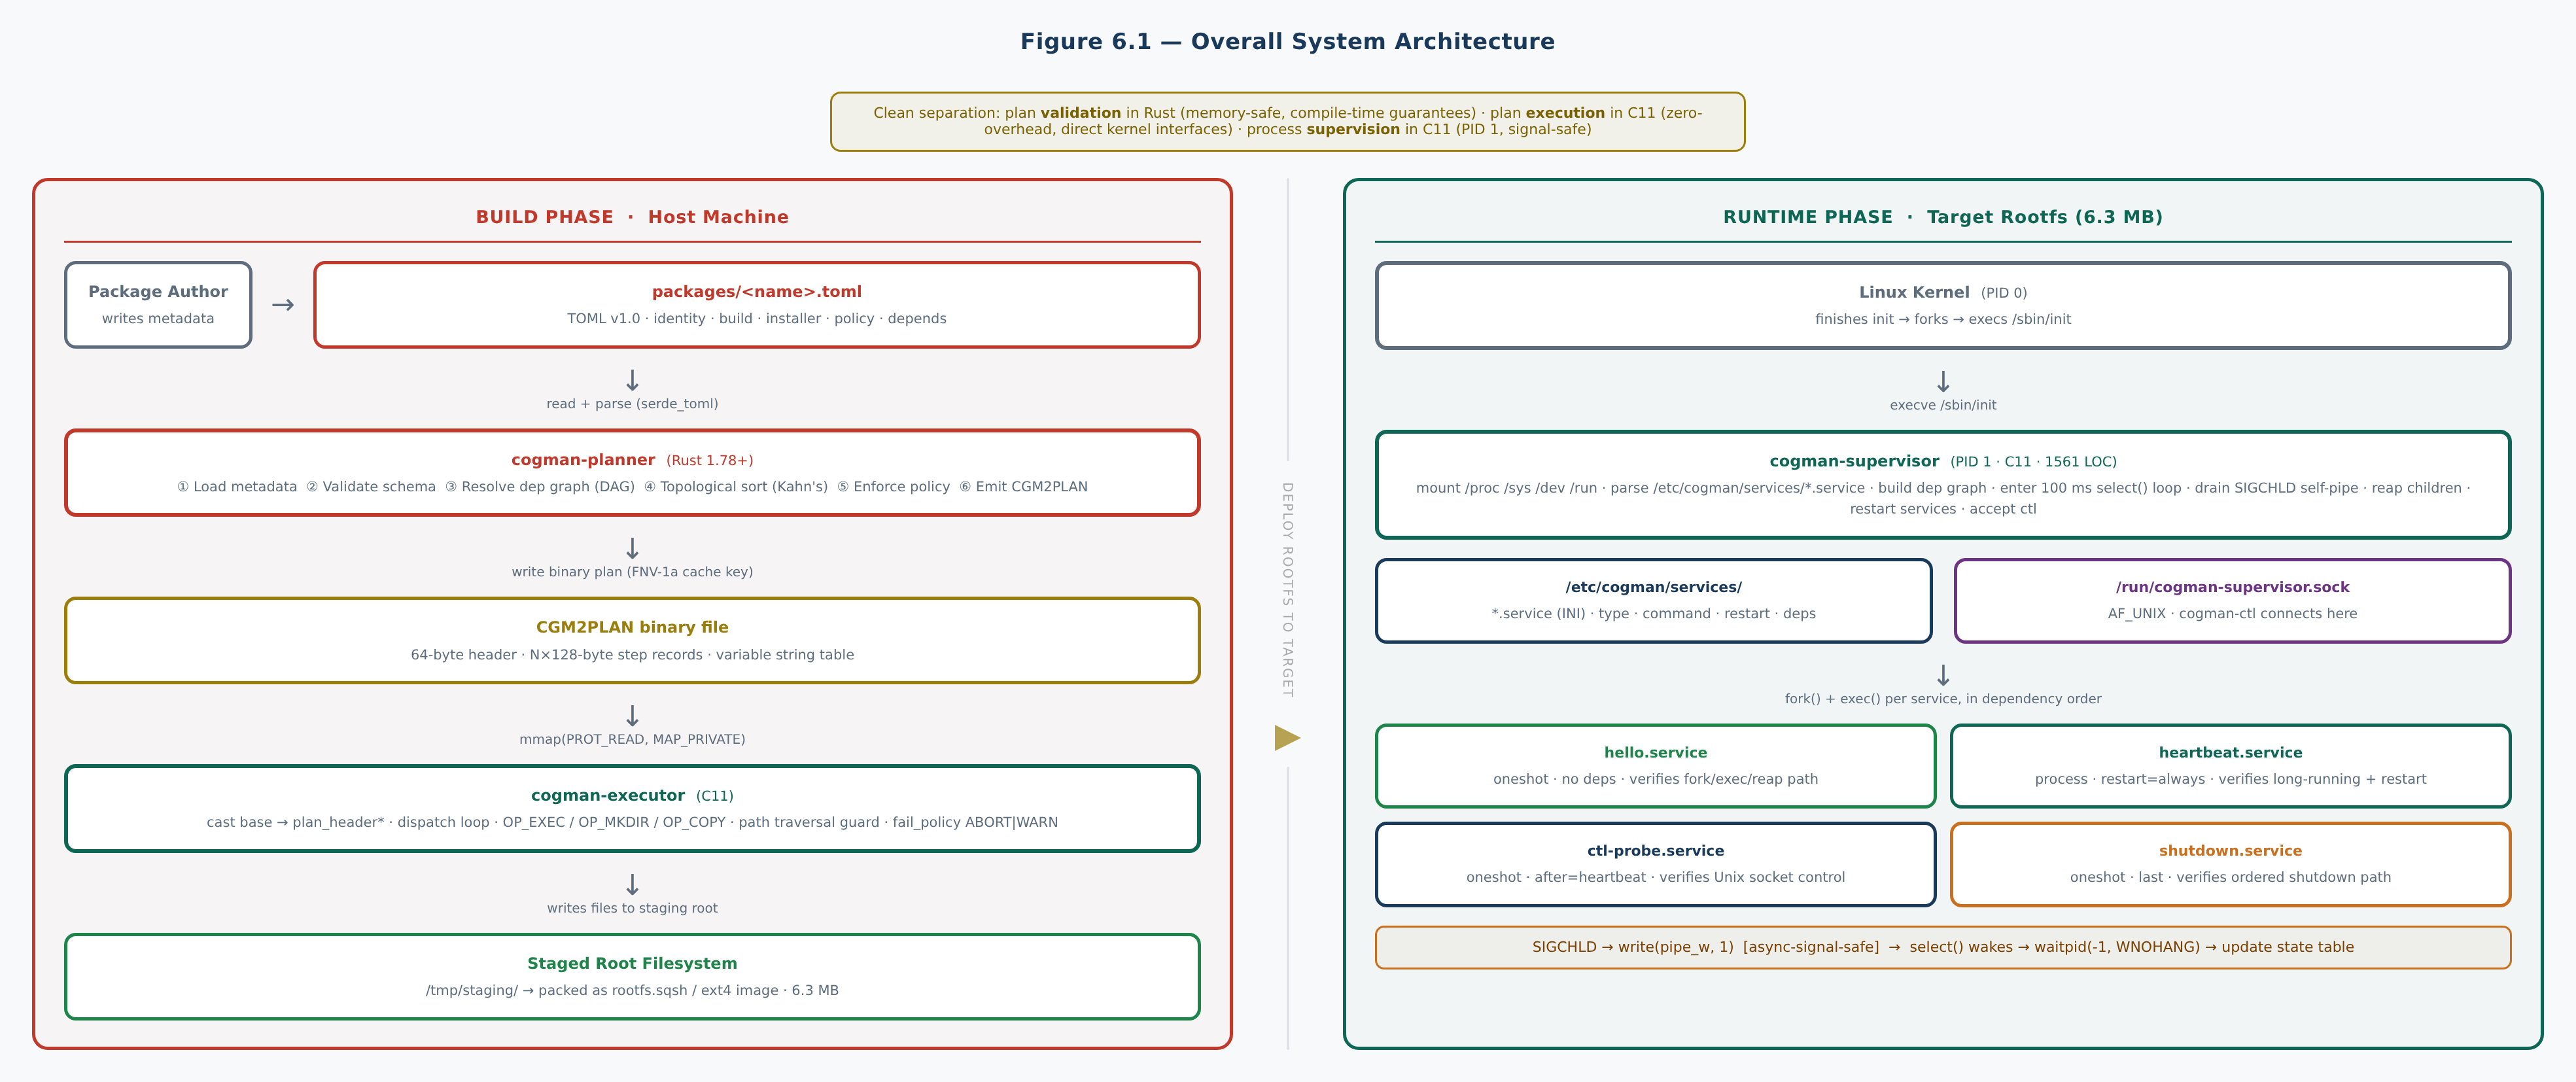
\includegraphics[width=0.92\textwidth]{fig6_1_system_arch.png}
  \caption{System Architecture --- Cogman Build System and Init Architecture}
  \label{fig:sysarch}
\end{figure}

\section{CGM2PLAN Binary Format --- Detailed Layout}

\begin{figure}[H]
  \centering
  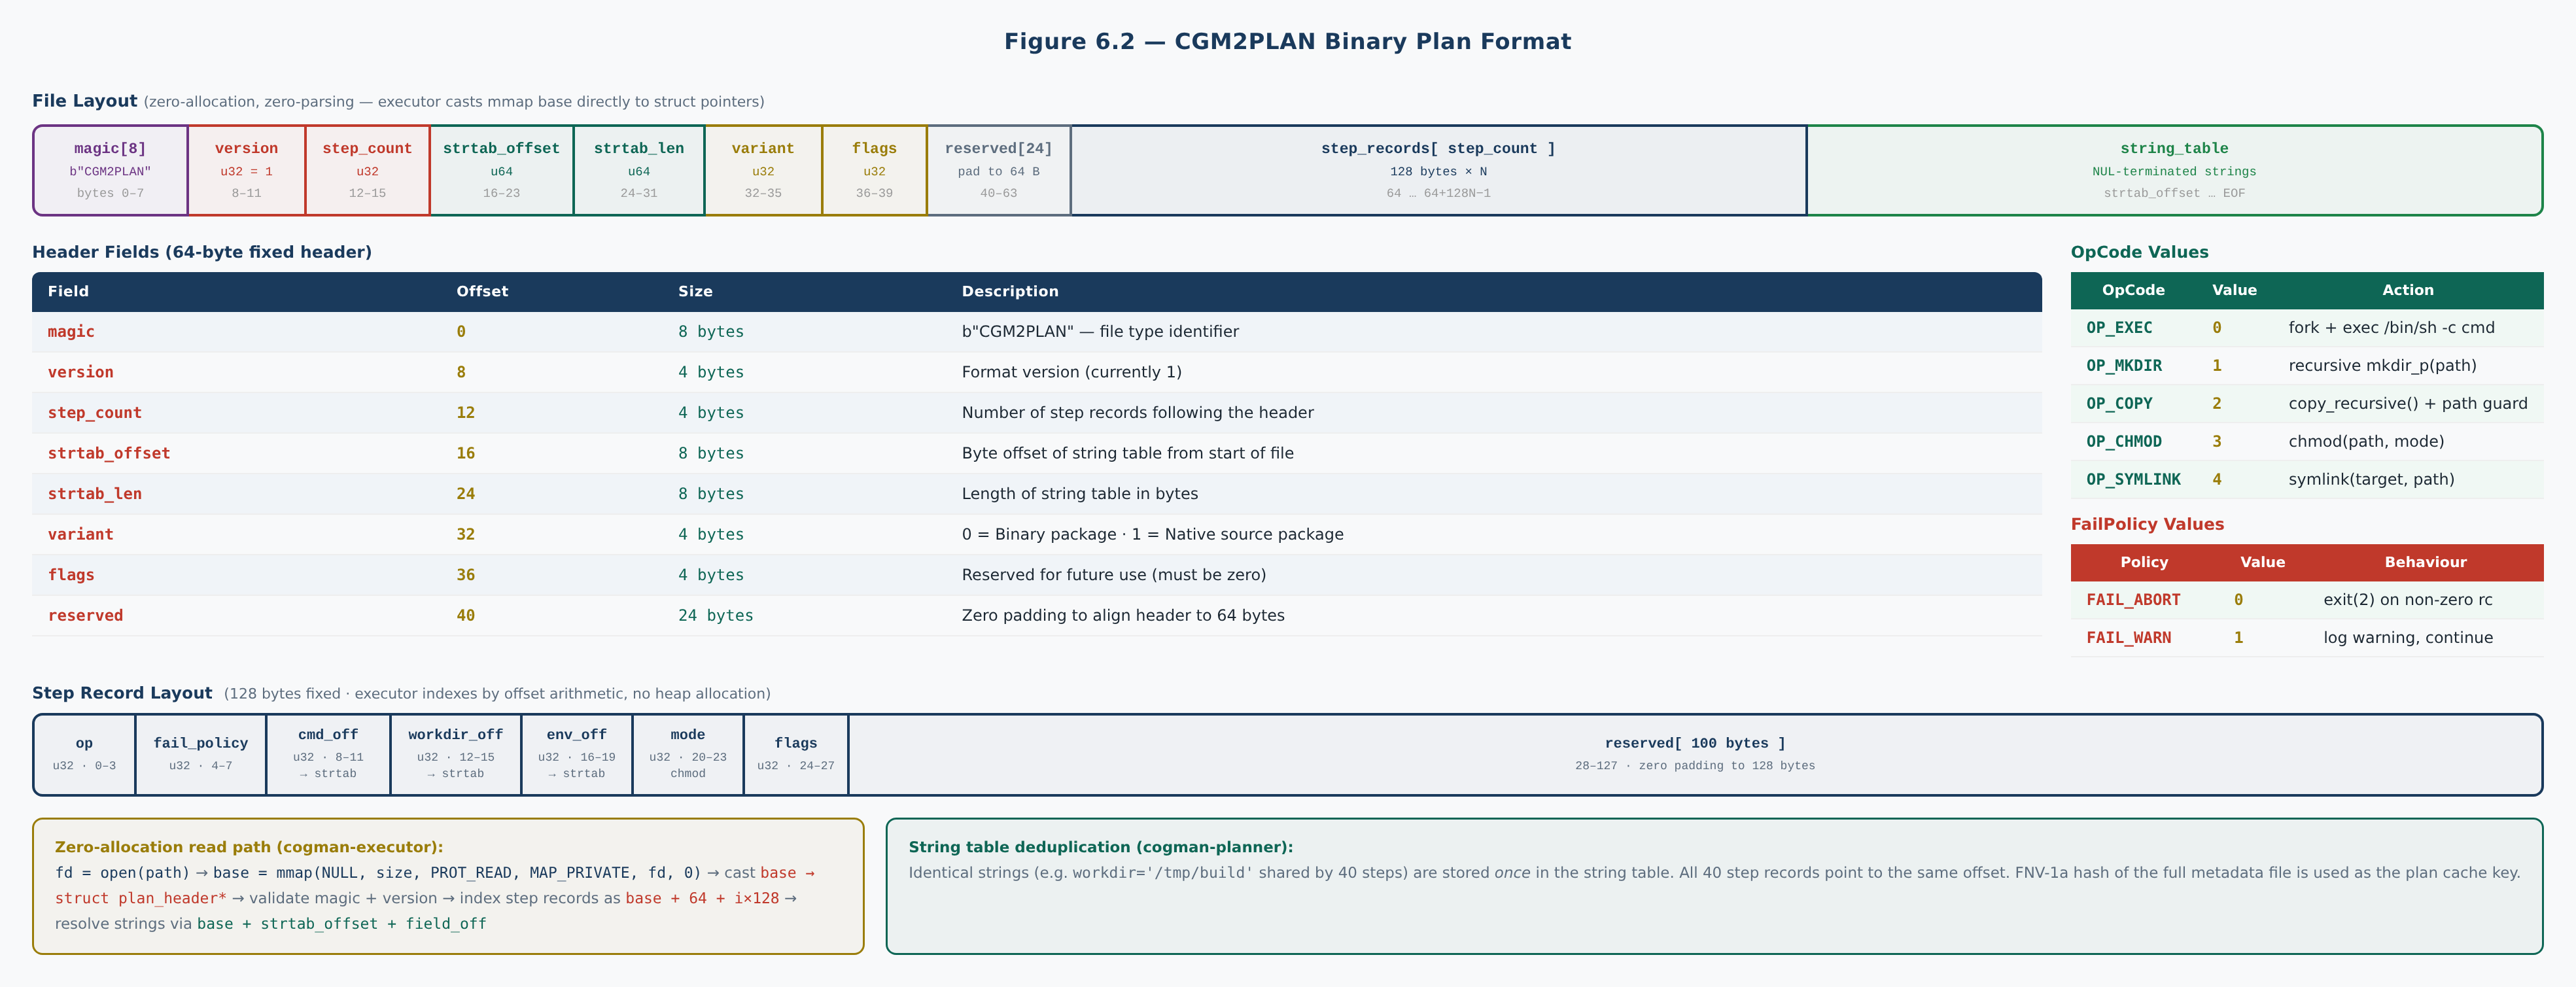
\includegraphics[width=0.88\textwidth]{fig6_2_cgm2plan_format.png}
  \caption{CGM2PLAN Binary Format --- Visual Layout showing Header, Step Records, and String Table}
  \label{fig:cgm2plan}
\end{figure}

\section{Data Flow Diagrams}

\subsection{DFD Level\,0 --- Context Diagram}

The Level\,0 DFD (Figure~\ref{fig:dfd0}) shows two external actors:
\textit{Package Author} (writes \texttt{package.toml} files and places source
archives) and \textit{System Operator} (invokes \texttt{cogman-planner} and
\texttt{cogman-executor} for builds; uses \texttt{cogman-ctl} for runtime
control). The system boundary encompasses four internal components:
\texttt{cogman-planner}, \texttt{cogman-executor}, \texttt{cogman-supervisor},
and \texttt{cogman-ctl}.

\begin{figure}[H]
  \centering
  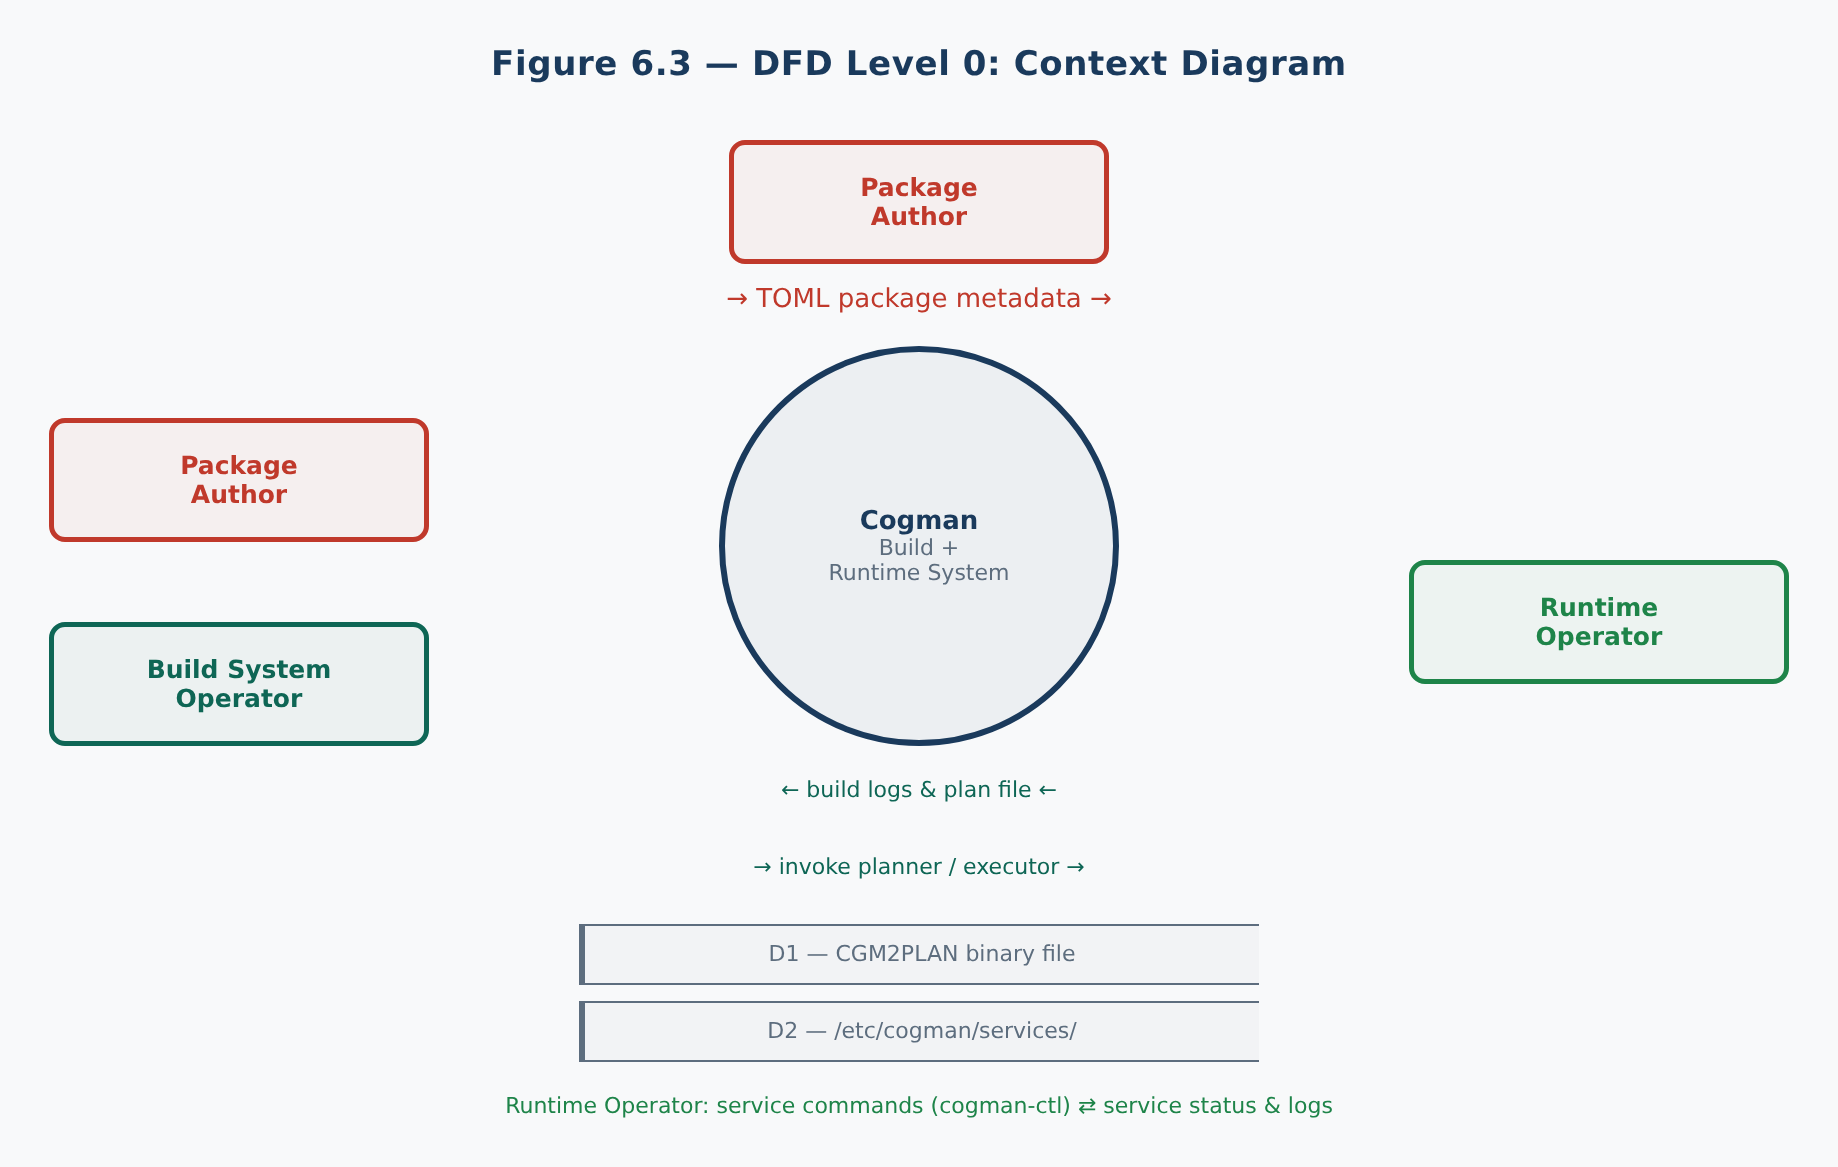
\includegraphics[width=0.88\textwidth]{fig6_3_dfd_level0.png}
  \caption{DFD Level\,0 --- Context Diagram}
  \label{fig:dfd0}
\end{figure}

\subsection{DFD Level\,1 --- Build Subsystem}

\begin{figure}[H]
  \centering
  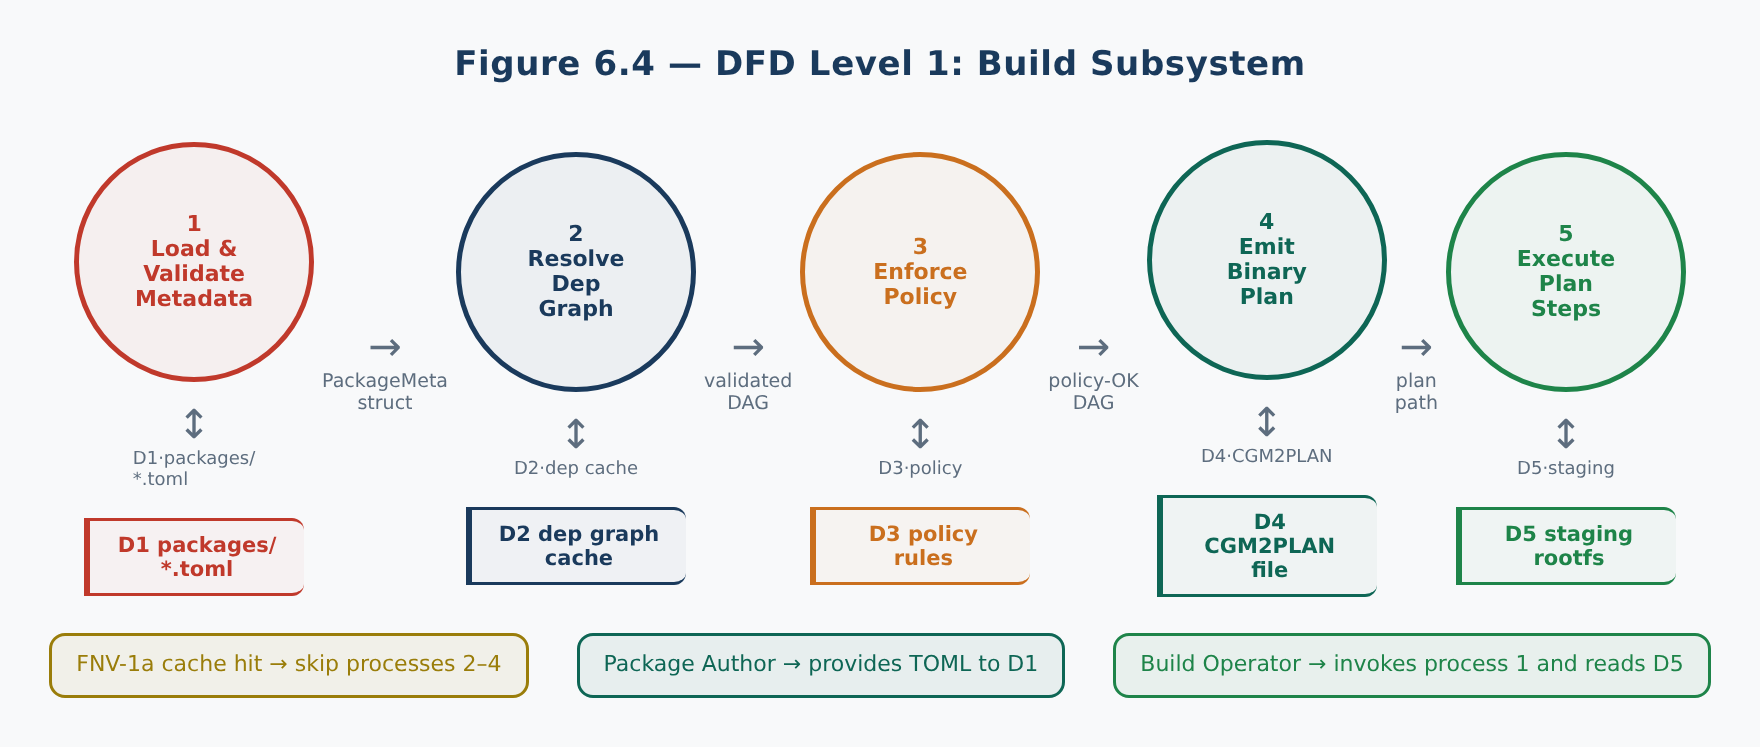
\includegraphics[width=0.88\textwidth]{fig6_4_dfd_level1.png}
  \caption{DFD Level\,1 --- Build Subsystem showing seven internal processes}
  \label{fig:dfd1}
\end{figure}

\begin{table}[H]
\centering
\caption{DFD Level\,1 Process Summary}
\renewcommand{\arraystretch}{1.2}
\begin{tabularx}{\linewidth}{l X X X}
\toprule
\textbf{Process} & \textbf{Input} & \textbf{Output} & \textbf{Data Store}\\
\midrule
P1: Schema Validation  & \texttt{package.toml} bytes     & PackageMetadata struct      & ---\\
P2: Dependency Loading & PackageMetadata, packages/       & DependencyGraph             & D1: packages/\\
P3: Cycle Detection    & DependencyGraph                  & Error or Ok                 & ---\\
P4: Topological Sort   & Acyclic DependencyGraph          & Ordered build list          & ---\\
P5: Policy Check       & PackageMetadata, rootfs path     & Error or Ok                 & ---\\
P6: Plan Emission      & Ordered steps, string table      & \texttt{build-plan.bin}     & D2: cache\\
P7: Step Execution     & \texttt{build-plan.bin} (mmap'd) & Files in \texttt{\$PKGROOT} & D3: rootfs\\
\bottomrule
\end{tabularx}
\end{table}

\section{Use Case Diagrams}

\begin{figure}[H]
  \centering
  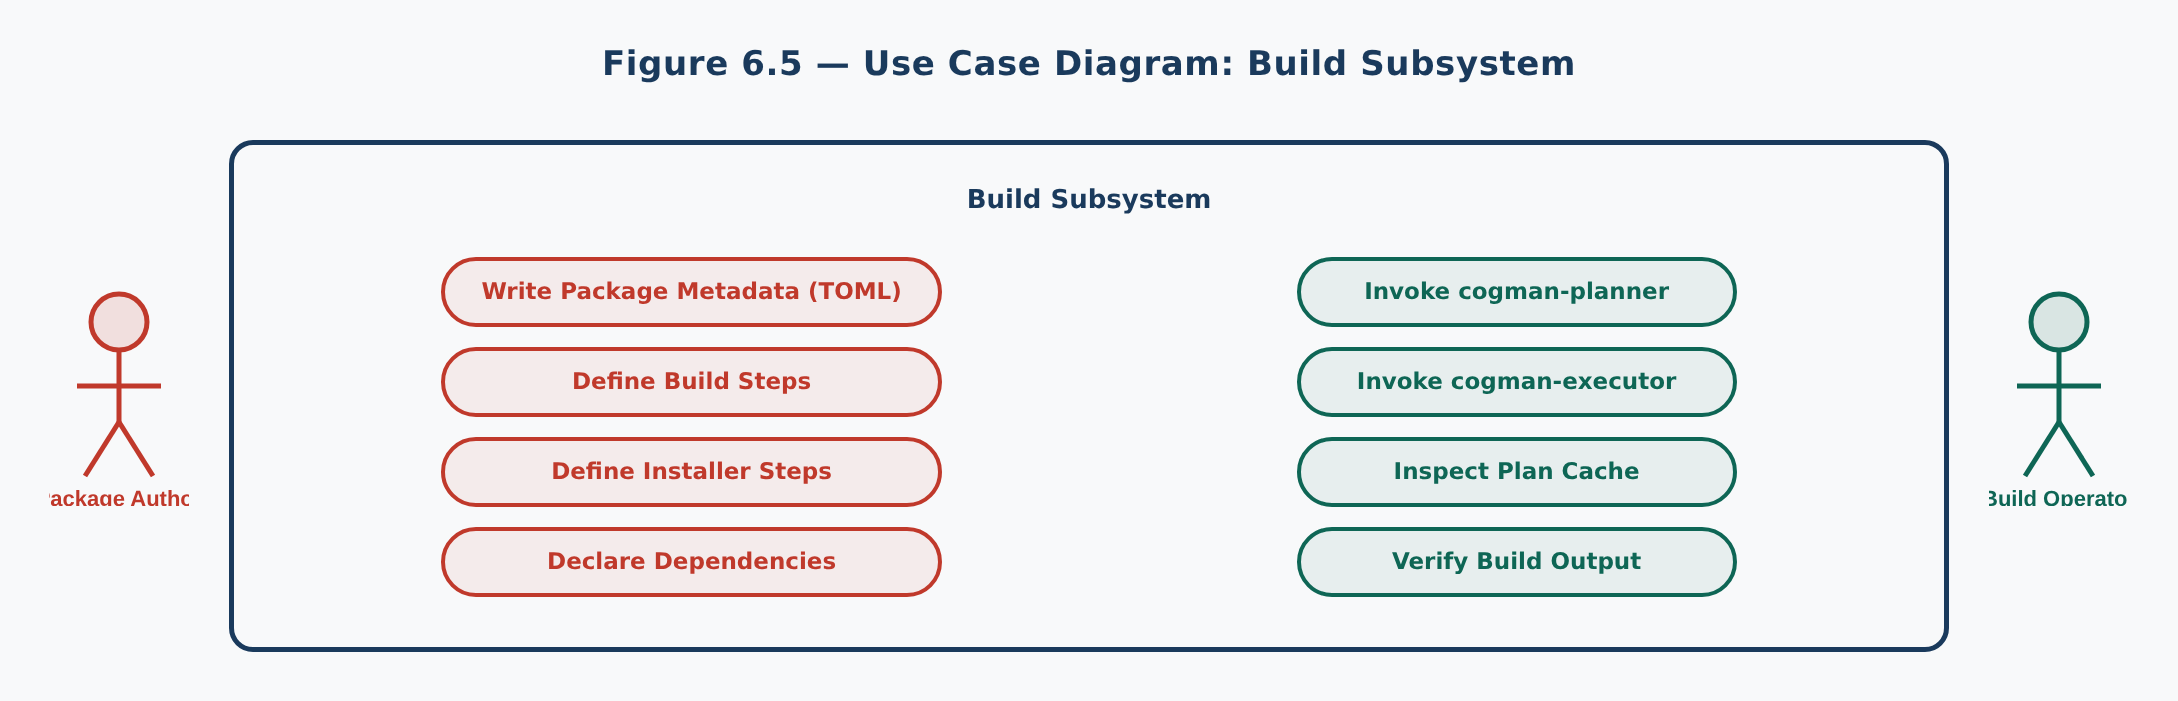
\includegraphics[width=0.85\textwidth]{fig6_5_usecase_build.png}
  \caption{Use Case Diagram --- Build Subsystem}
  \label{fig:usecase_build}
\end{figure}

\begin{figure}[H]
  \centering
  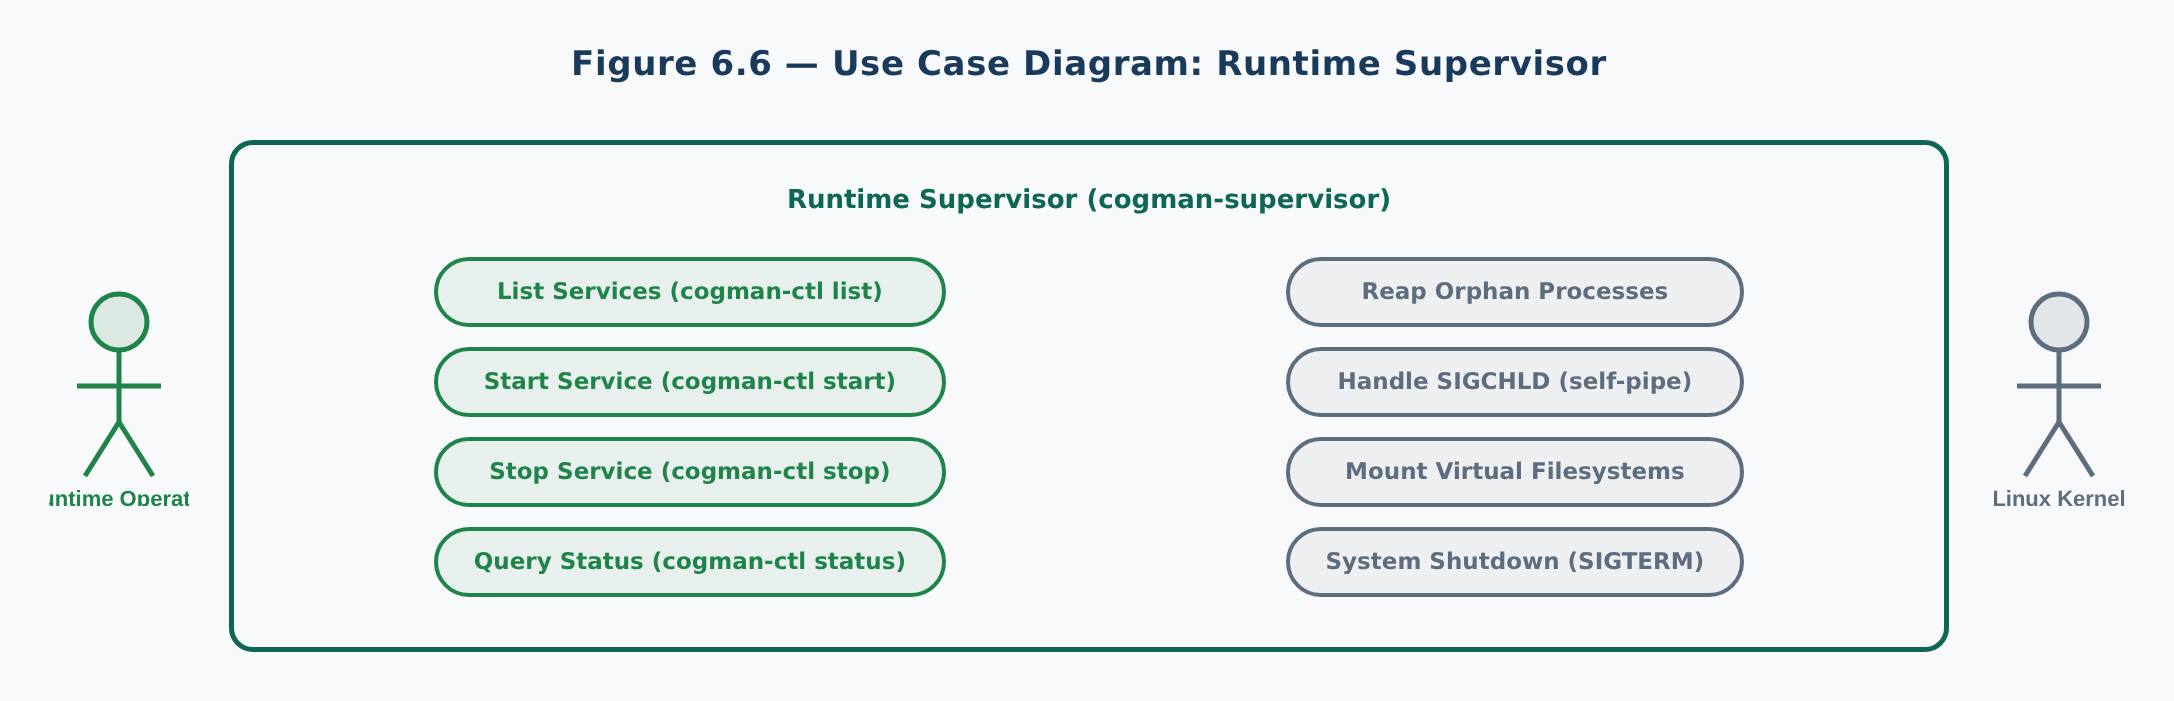
\includegraphics[width=0.85\textwidth]{fig6_6_usecase_runtime.png}
  \caption{Use Case Diagram --- Runtime Subsystem}
  \label{fig:usecase_runtime}
\end{figure}

The Build Subsystem use case shows two actors: \textit{Package Author} and
\textit{Build Engineer}. Package Authors define package metadata, declare build
steps, declare dependencies, and set security policy. Build Engineers invoke the
planner, invoke the executor, and verify the staging rootfs. The system enforces
schema validation on planner invocation, cycle detection on dependency load, policy
check before plan emission, and path traversal guard on every \texttt{OP\_COPY}
execution. The Runtime Subsystem use case shows the \textit{System Operator}
interacting with \texttt{cogman-ctl} to start, stop, restart, and query services;
the supervisor enforces dependency ordering and restart policy automatically.

\subsection{Security Constraints at Use Case Boundaries}

Each use case in both subsystems is bounded by security constraints that the
system enforces automatically, without relying on operator vigilance. At the
\textit{Invoke Planner} boundary, the TOML schema validator rejects malformed
metadata before any graph construction begins, ensuring that malformed package
definitions cannot propagate into the dependency resolution stage. At the
\textit{Invoke Executor} boundary, the path traversal guard
(\texttt{path\_has\_traversal()}) is called for every \texttt{OP\_COPY} step
before the destination file descriptor is opened, preventing any plan --- even a
manually crafted one --- from writing outside the declared staging rootfs. At the
\textit{Start/Stop/Restart Service} boundary, the UDS control socket accepts
connections only from processes with sufficient file descriptor access to the
socket path (\texttt{/run/cogman.sock}), and the command parser rejects
unrecognised commands with an explicit error response. At the \textit{Query
Service Status} boundary, the status response is constructed from in-memory
supervisor state and never executes shell commands, preventing injection attacks
through service name fields.

\begin{table}[H]
\centering
\caption{Use Cases, Actors, and Preconditions}
\label{tab:usecases}
\renewcommand{\arraystretch}{1.2}
\begin{tabularx}{\linewidth}{l l X X}
\toprule
\textbf{Use Case} & \textbf{Actor} & \textbf{Precondition} & \textbf{Security Guard}\\
\midrule
Invoke Planner   & Build Engineer    & Valid \texttt{package.toml} exists    & Schema validation; policy check\\
Invoke Executor  & Build Engineer    & \texttt{build-plan.bin} present; rootfs writable & Path traversal guard per step\\
Start Service    & System Operator   & Supervisor running; service file present & Dependency gate; UDS auth\\
Query Status     & System Operator   & UDS socket accessible (\texttt{/run/cogman.sock}) & Read-only state snapshot\\
\bottomrule
\end{tabularx}
\end{table}

\clearpage
\section{Class Diagrams}

\begin{figure}[H]
  \centering
  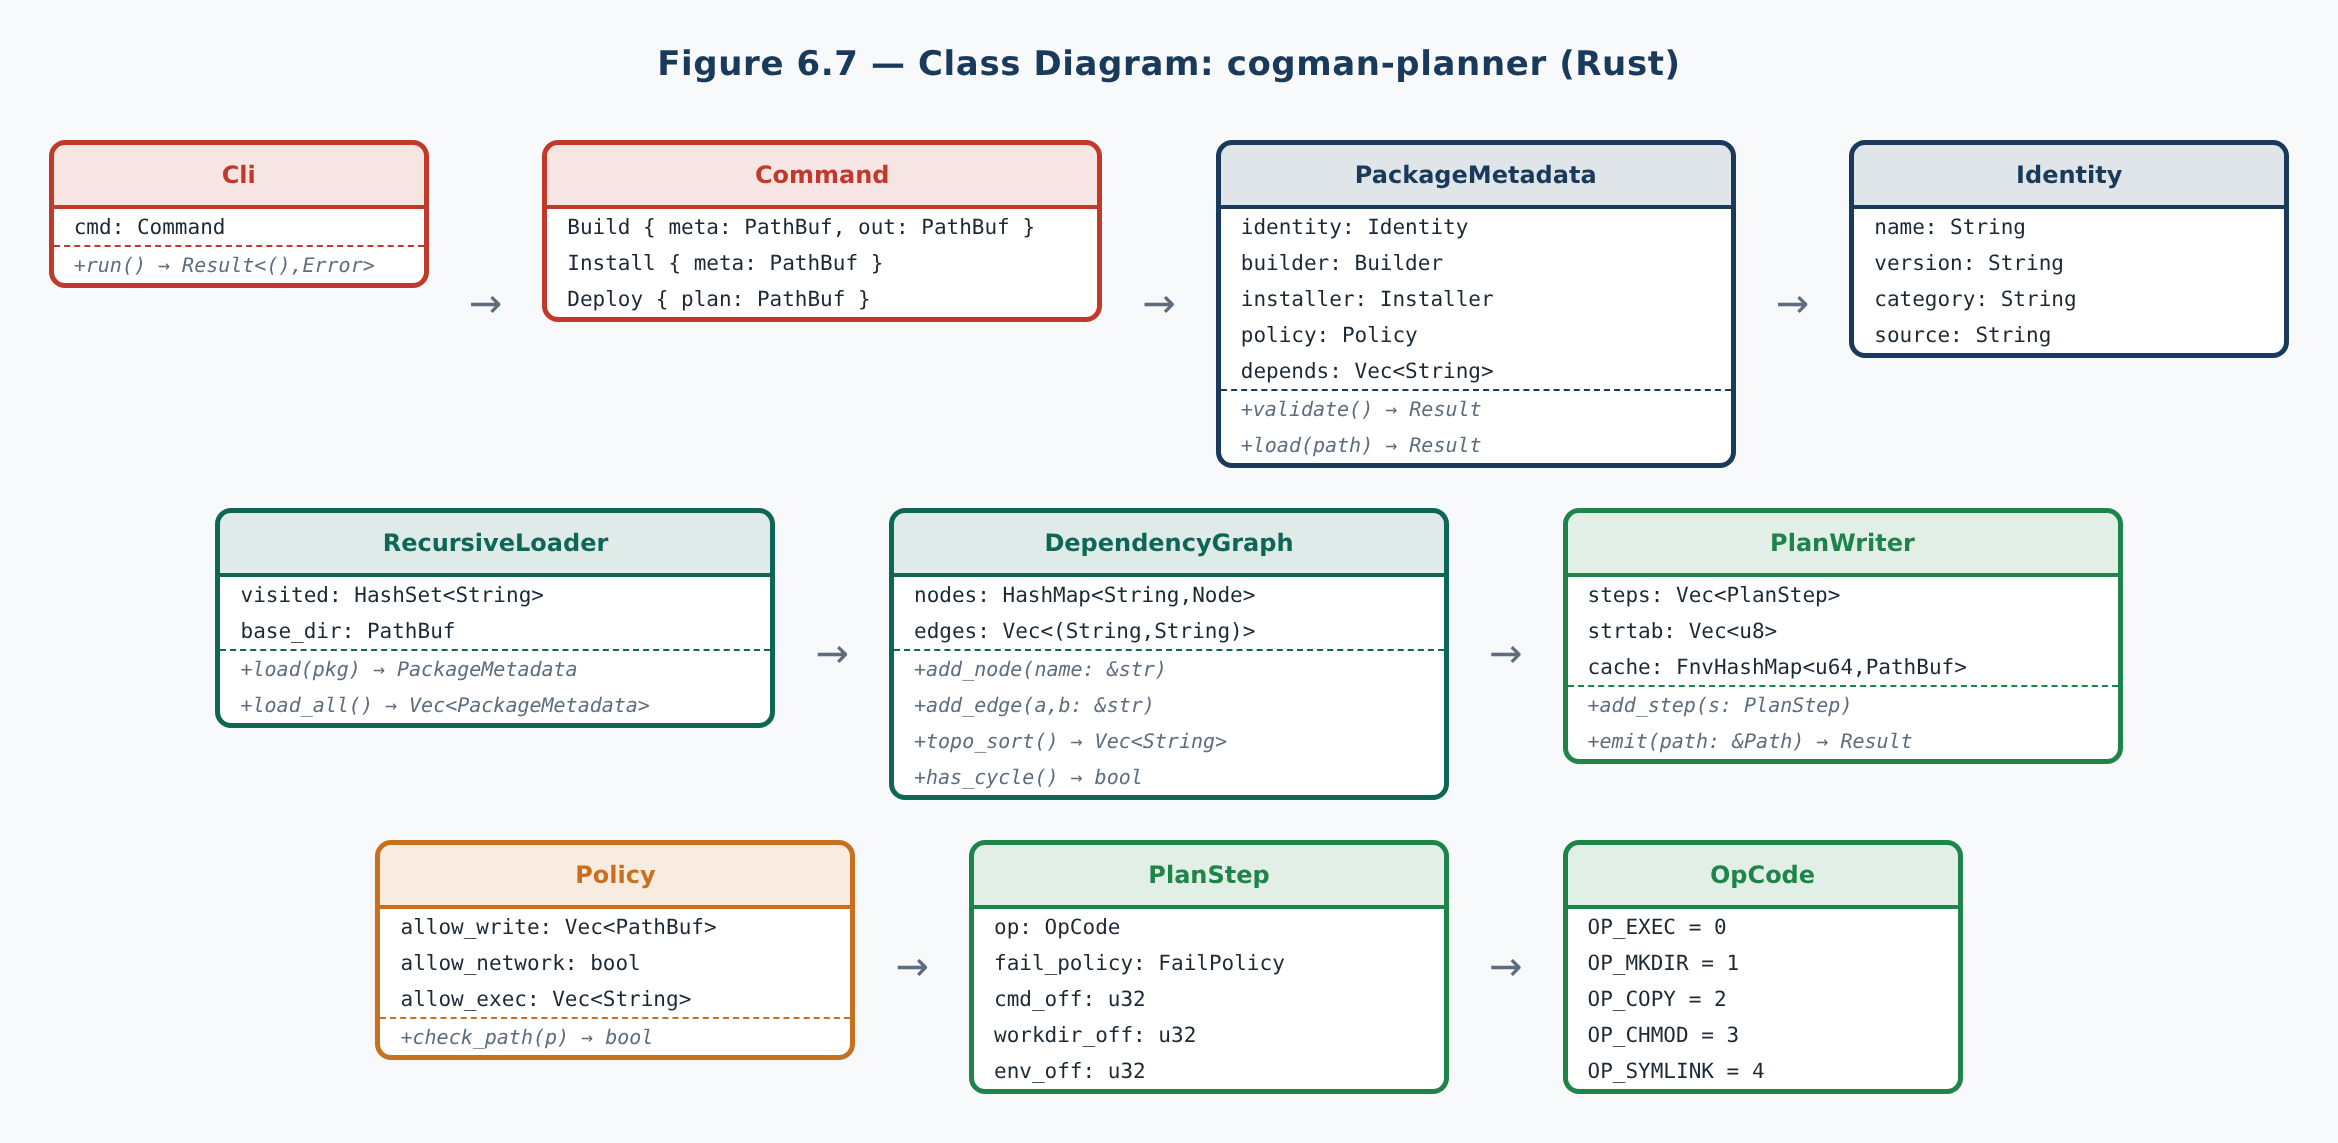
\includegraphics[width=0.85\textwidth]{fig6_7_class_planner.png}
  \caption{Class Diagram --- cogman-planner}
  \label{fig:class_planner}
\end{figure}

\begin{figure}[H]
  \centering
  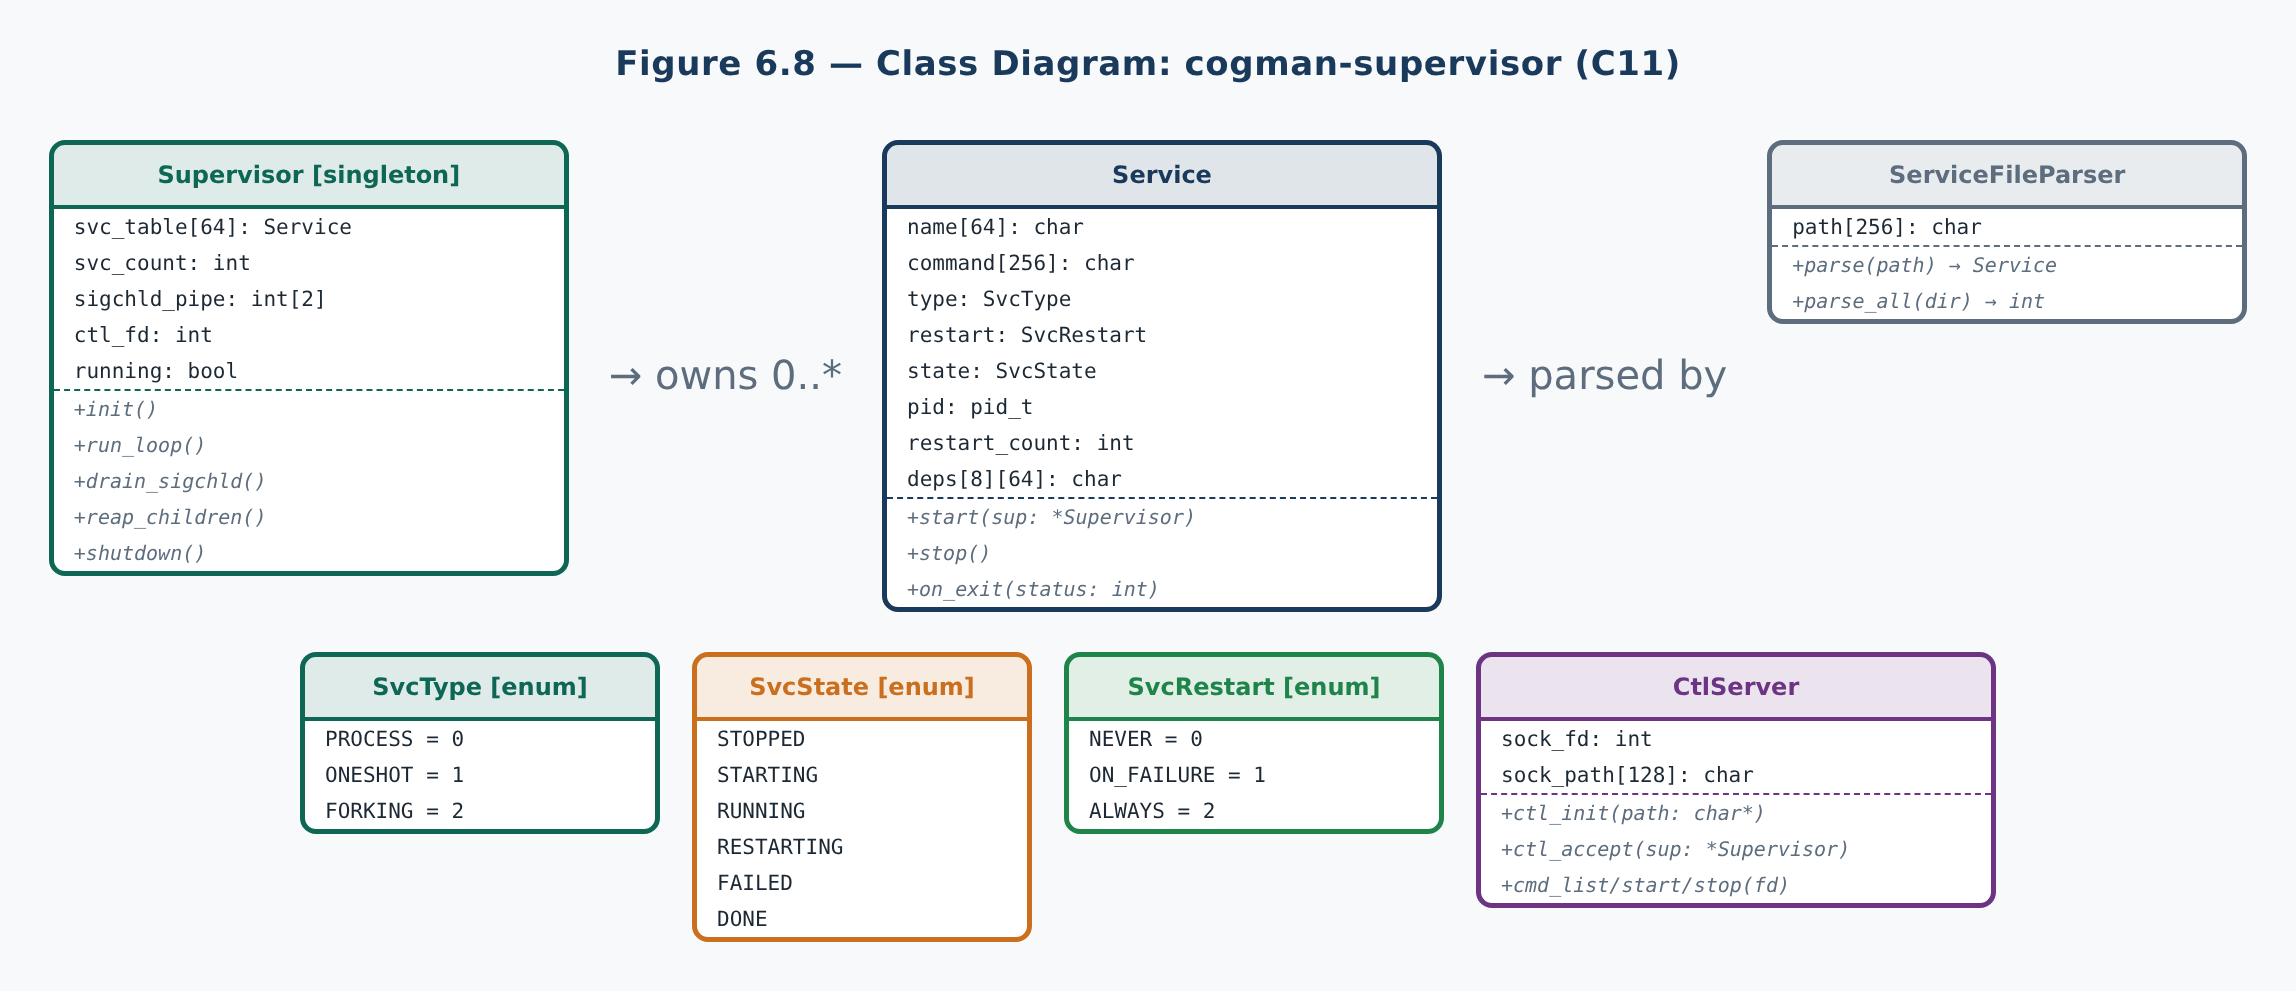
\includegraphics[width=0.85\textwidth]{fig6_8_class_supervisor.png}
  \caption{Class Diagram --- cogman-supervisor}
  \label{fig:class_supervisor}
\end{figure}

The cogman-planner class diagram shows the primary structs: \texttt{PackageMetadata}
(aggregating \texttt{Identity}, \texttt{Builder}, \texttt{Installer},
\texttt{Policy}), \texttt{DependencyGraph} (HashMap-based adjacency list), and
\texttt{PlanEmitter} (CGM2PLAN binary writer with string table deduplication).
The cogman-supervisor class diagram shows the \texttt{service} struct (containing
name, pid, state, restart policy, restart\_at, depends\_on), the supervisor state
machine (\texttt{sup\_tick()}, \texttt{sup\_handle\_dead()}), and the UDS control
handler (\texttt{ctl\_dispatch()}).

\section{Sequence Diagrams}

\begin{figure}[H]
  \centering
  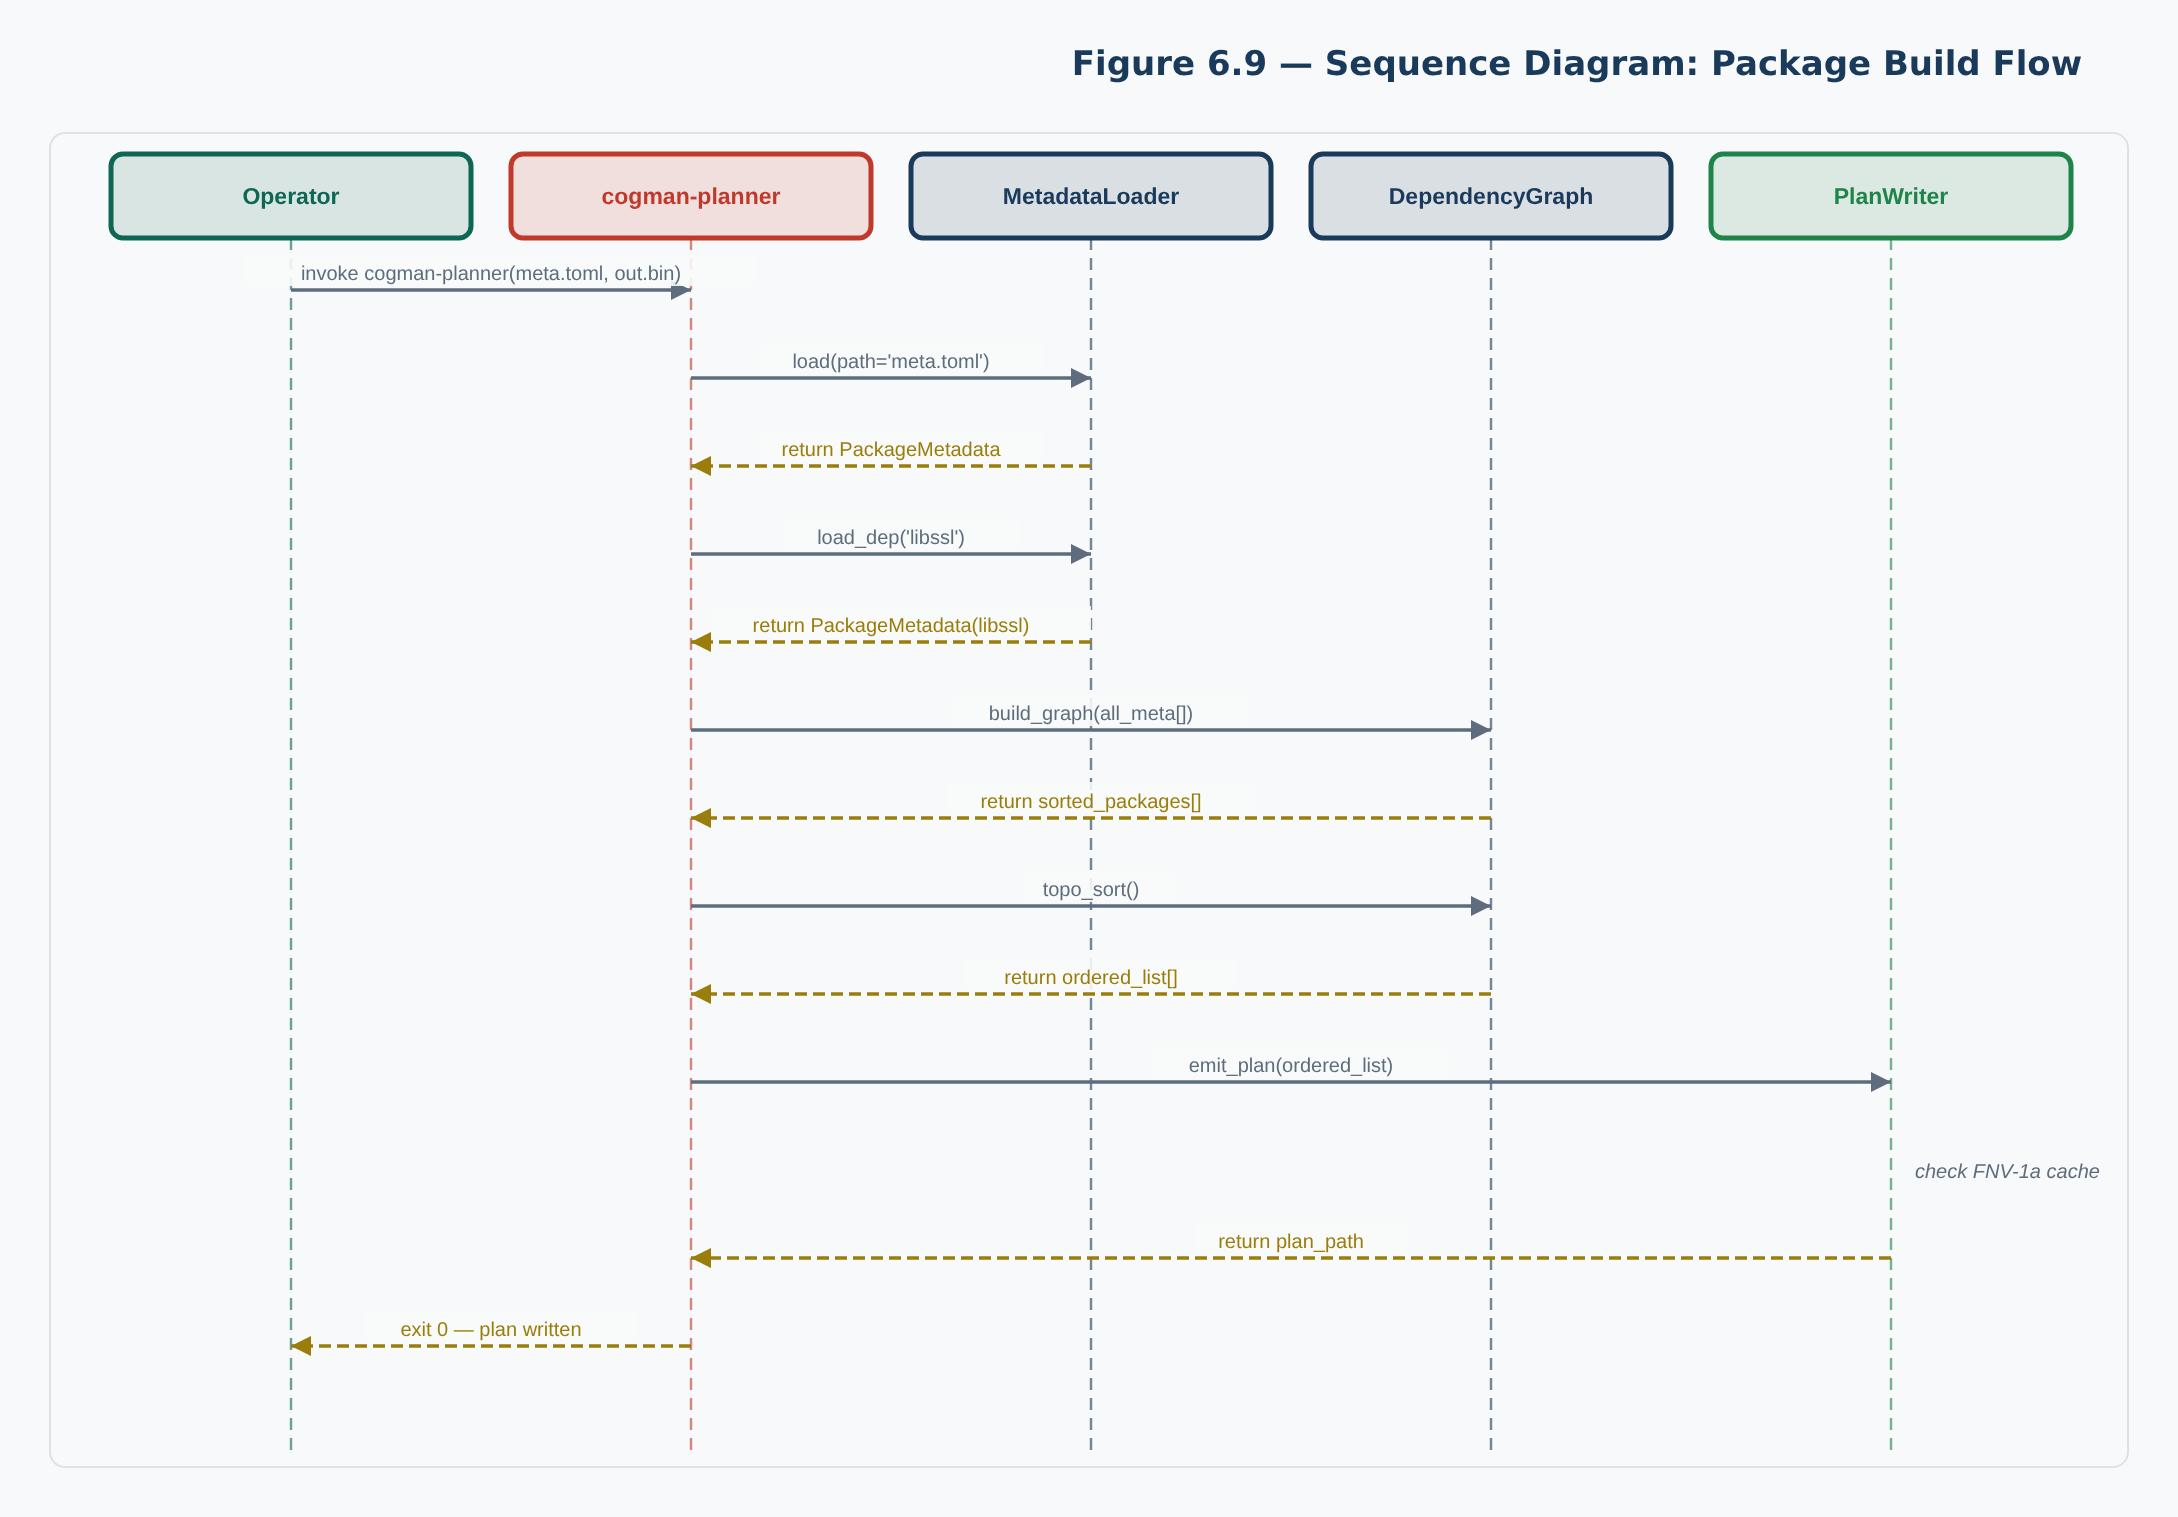
\includegraphics[width=0.85\textwidth]{fig6_9_seq_build.png}
  \caption{Sequence Diagram --- Build Flow}
  \label{fig:seq_build}
\end{figure}

\begin{figure}[H]
  \centering
  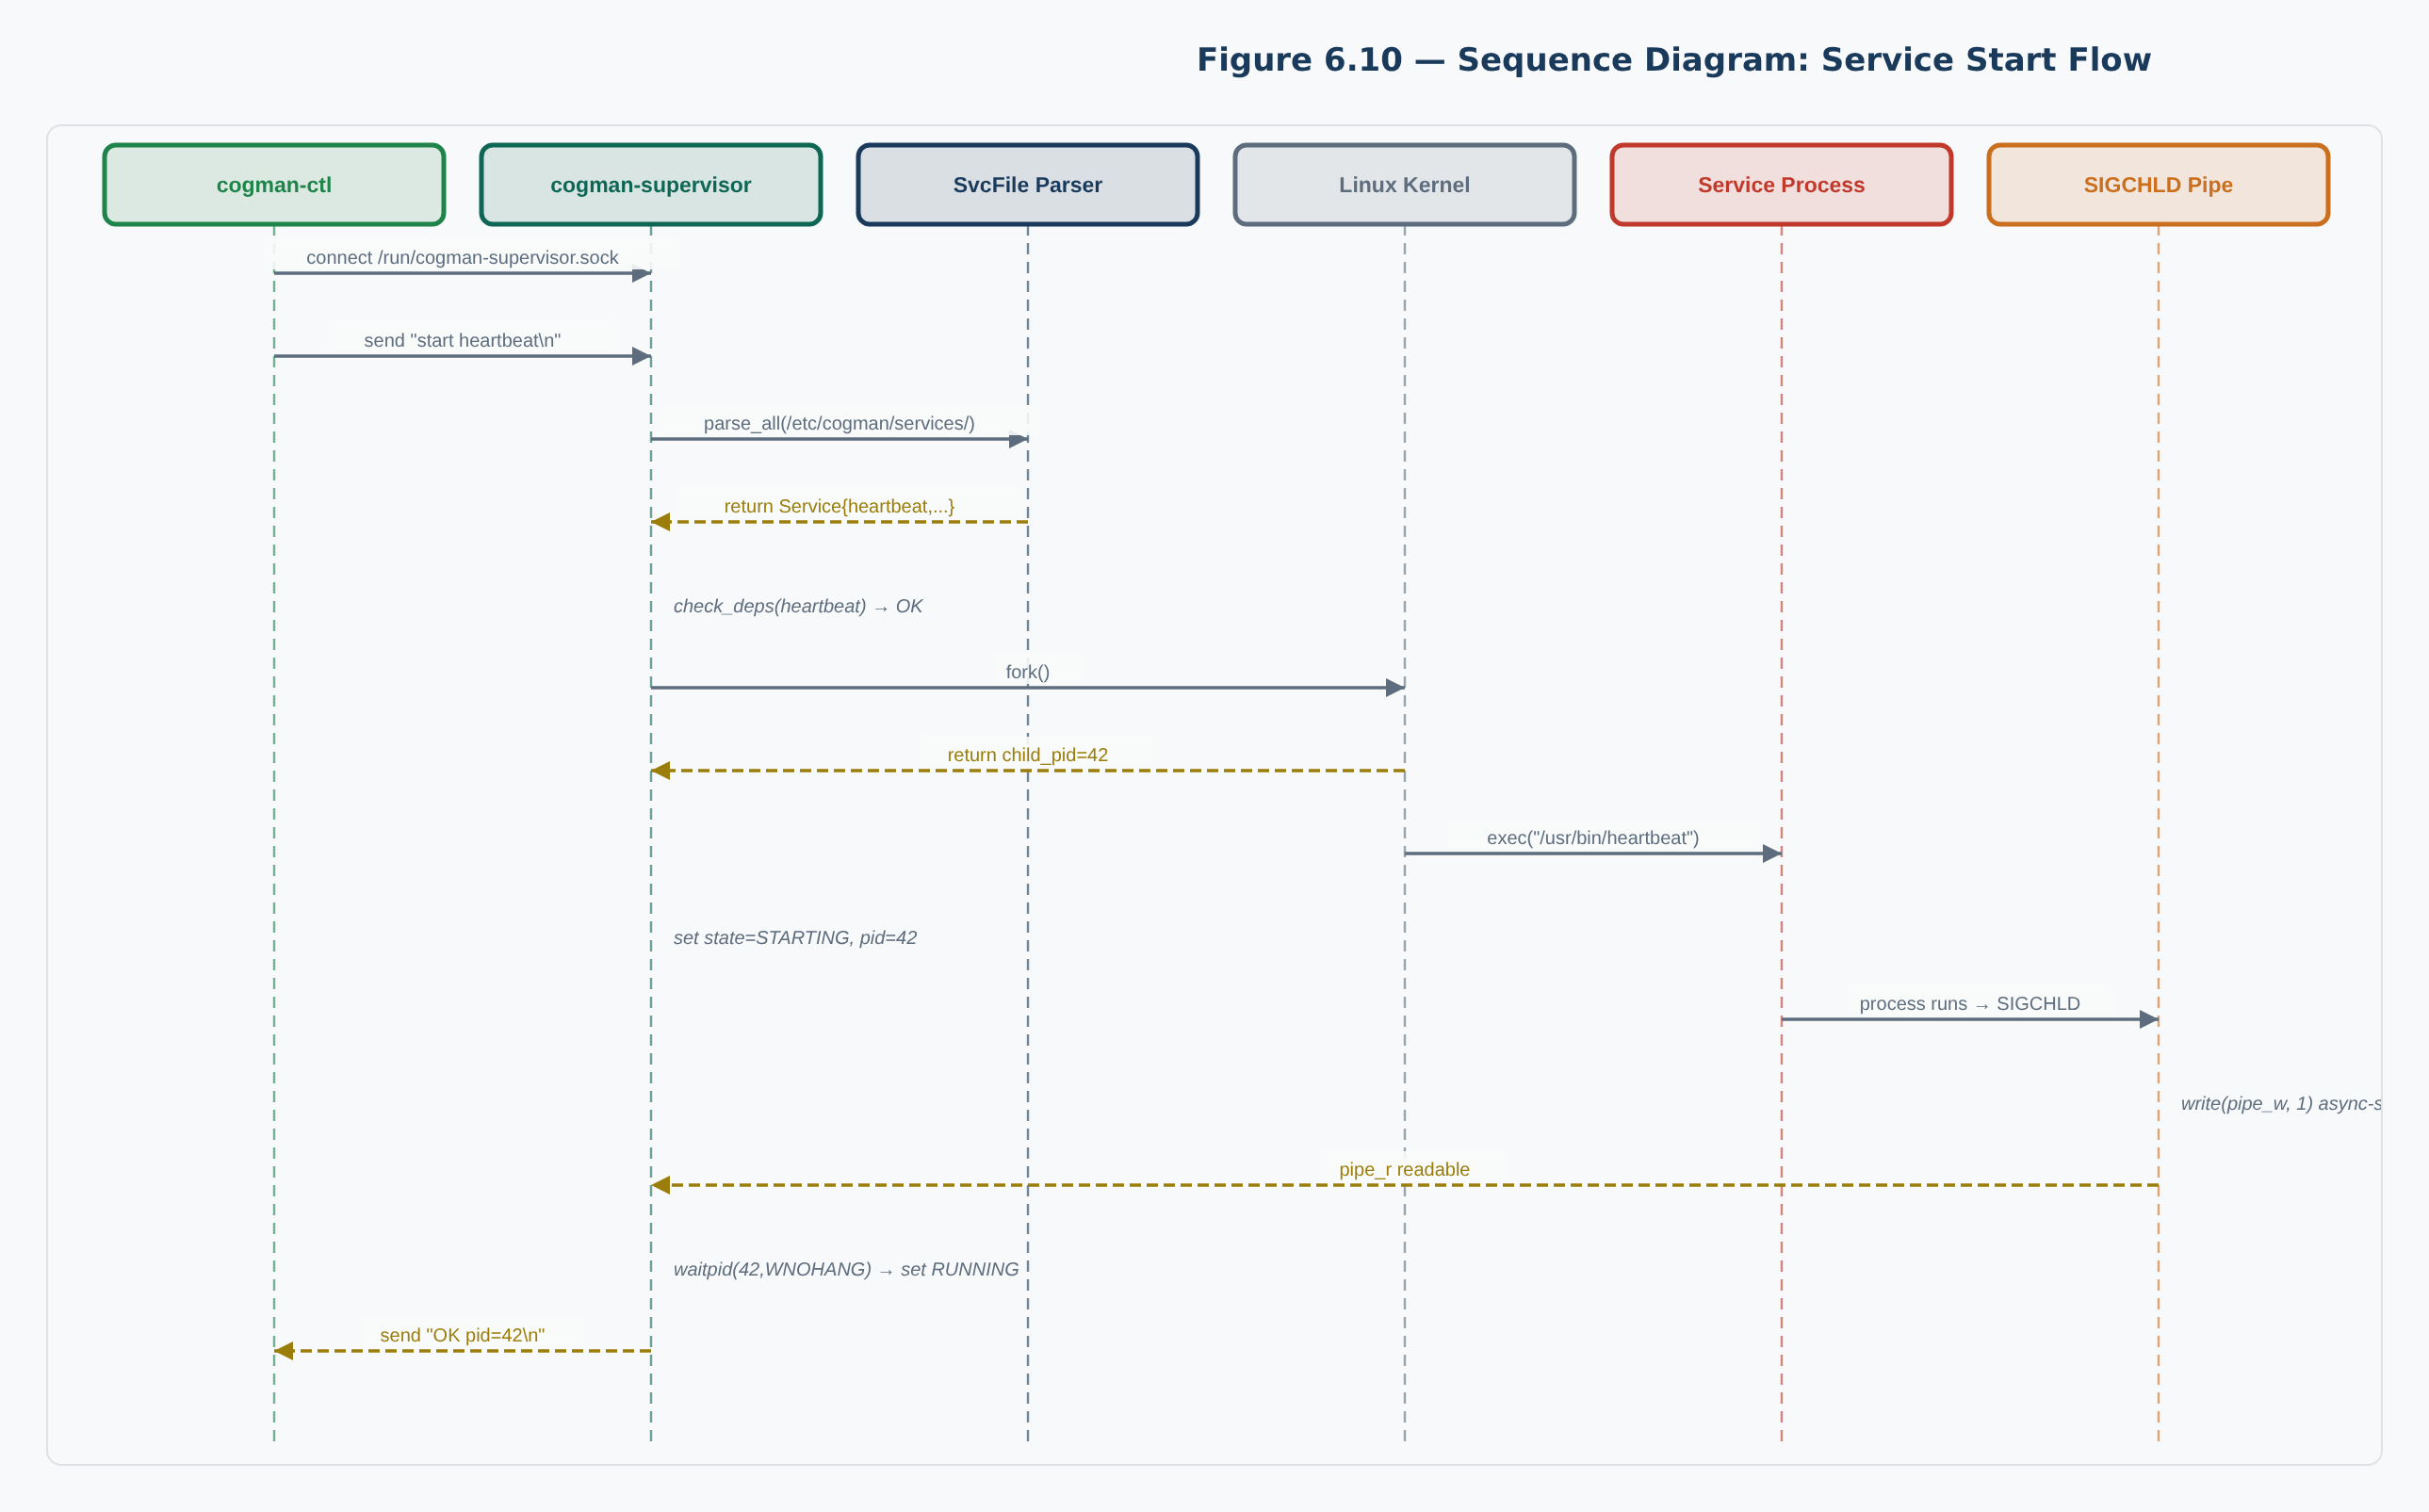
\includegraphics[width=0.85\textwidth]{fig6_10_seq_start.png}
  \caption{Sequence Diagram --- Supervisor Start}
  \label{fig:seq_start}
\end{figure}

\clearpage
The build flow sequence diagram shows twelve interactions from planner invocation
to executor exit: (1) \texttt{plan --input pkg.toml}, (2)
\texttt{load\_and\_validate()}, (3) \texttt{load\_deps()}, (4)
\texttt{detect\_cycles()}, (5) \texttt{topological\_sort()}, (6)
\texttt{check\_policy()}, (7) \texttt{emit\_plan()} producing
\texttt{build-plan.bin}, (8) \texttt{mmap(build-plan.bin)}, (9)
\texttt{validate\_header()}, (10) per-step \texttt{fork()+execve()}, (11)
\texttt{waitpid()}, (12) \texttt{exit(0)}. The supervisor start sequence shows
service loading from \texttt{/etc/cogman/services/}, dependency gate evaluation,
SIGCHLD pipe setup, and entry into the \texttt{select()} main loop.

\section{Component Diagram}

\begin{figure}[H]
  \centering
  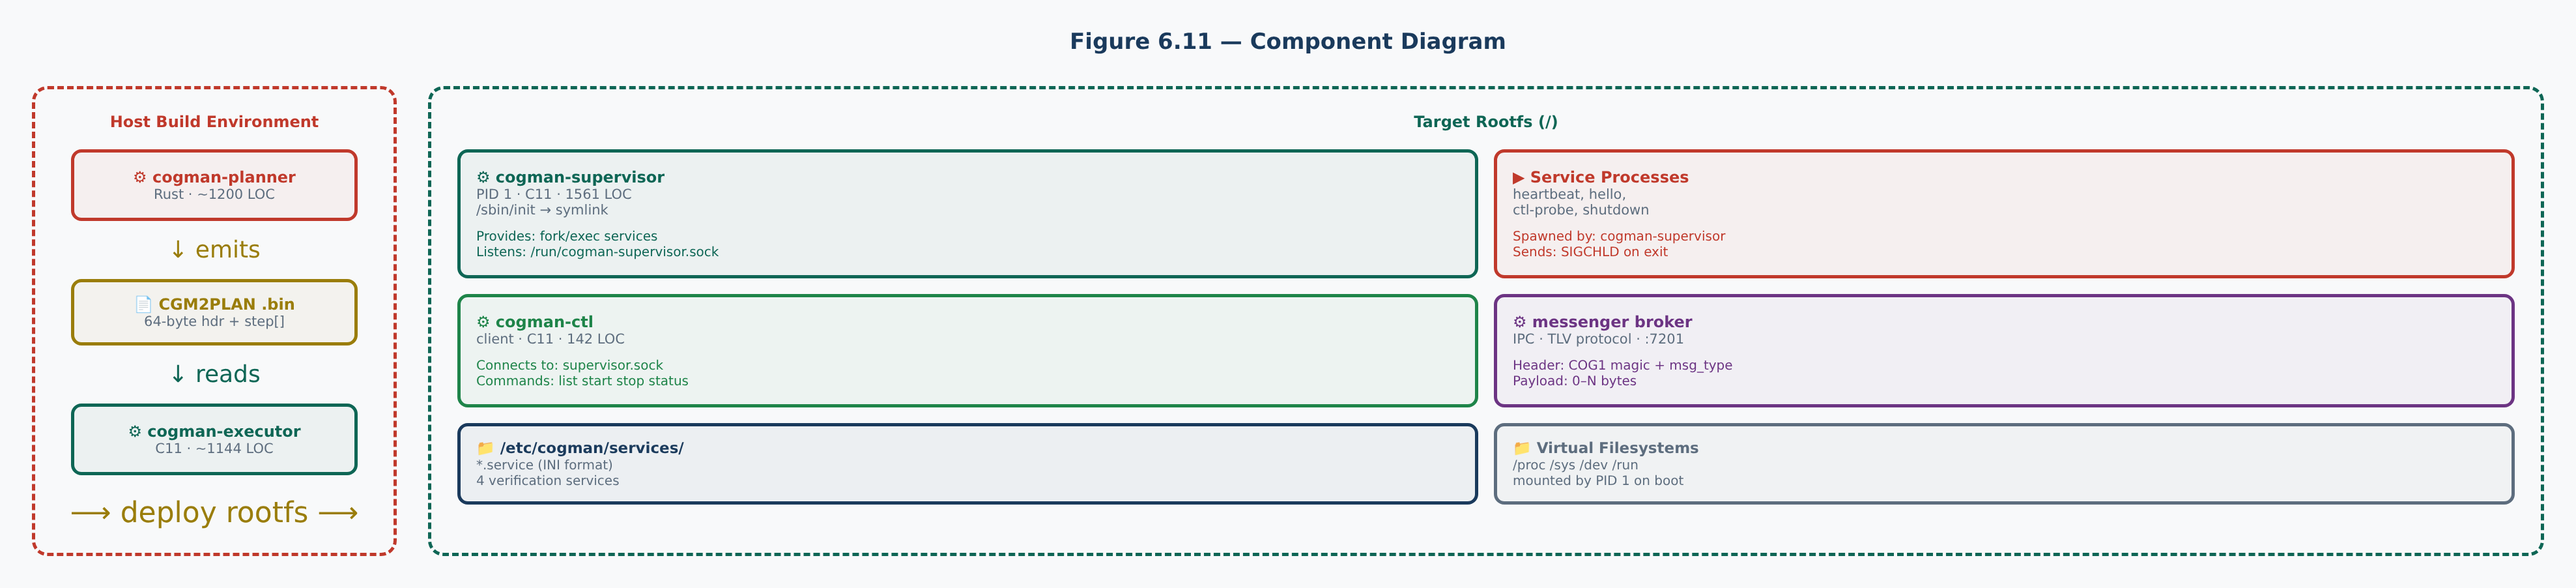
\includegraphics[width=0.88\textwidth]{fig6_11_component.png}
  \caption{Component Diagram --- Cogman binary interfaces and data flows}
  \label{fig:component}
\end{figure}

The component diagram shows the four Cogman binaries and their interfaces: the
CGM2PLAN file interface between planner and executor, the UDS socket interface
between supervisor and ctl, the INI service definition file interface consumed by
the supervisor at boot, and the Messenger IPC interface between the supervisor and
the AI advisor. The AI advisor connects to the planner's log output and the
operator's query interface but has no write access to any system state.

The diagram highlights two properties of the Cogman architecture. First, every
inter-component interface is a file or socket on the local filesystem --- CGM2PLAN
files in \texttt{/var/cache/cogman/}, service definition files in
\texttt{/etc/cogman/services/}, and Unix domain sockets in \texttt{/run/} ---
making the entire communication model inspectable with standard POSIX tools
(\texttt{ls}, \texttt{xxd}, \texttt{socat}) without any proprietary client software.
Second, the build half (planner and executor) and the runtime half (supervisor and
ctl) share no in-memory state: their only coupling is through the on-disk CGM2PLAN
file, meaning either half can be upgraded, restarted, or replaced without affecting
the other. This clean separation is essential for a security distribution where
each component's privilege level and filesystem access must be independently
auditable and minimisable.

\section{Service Lifecycle State Machine}

\begin{table}[H]
\centering
\caption{Service State Machine Transitions}
\renewcommand{\arraystretch}{1.2}
\begin{tabularx}{\linewidth}{l X l}
\toprule
\textbf{From State} & \textbf{Trigger} & \textbf{To State}\\
\midrule
STOPPED     & Dependency gate open, scheduled start     & STARTING\\
STARTING    & Process forked (pid $>$ 0)                & RUNNING\\
RUNNING     & Exited code 0, type=oneshot               & DONE\\
RUNNING     & Exited code $\neq$0, restart=never        & FAILED\\
RUNNING     & Exited, restart=always                    & RESTARTING\\
RUNNING     & Exited code $\neq$0, restart=on-failure   & RESTARTING\\
RESTARTING  & restart\_delay elapsed                    & STARTING\\
Any         & \texttt{cogman-ctl stop}                  & STOPPED\\
\bottomrule
\end{tabularx}
\end{table}

The service lifecycle state machine defines six distinct states. \textbf{STOPPED}
is the initial state for all services and the state entered upon receiving a
\texttt{cogman-ctl stop} command; a service in STOPPED does not consume CPU and
holds no file descriptors. \textbf{STARTING} indicates that the dependency gate
has been cleared and \texttt{fork()} has been called but the supervisor has not
yet received a SIGCHLD confirming the child's initial execution. \textbf{RUNNING}
is the normal operational state for longrun services and persists until the process
exits. \textbf{DONE} is the terminal success state for oneshot services that exit
with code\,0; no restart is attempted from DONE regardless of the configured
restart policy. \textbf{FAILED} is the terminal failure state reached when a
service exits with a non-zero code under a \texttt{restart=never} policy; the
operator must issue an explicit \texttt{cogman-ctl restart} command to re-enter
the STARTING state. \textbf{RESTARTING} is a transient state that prevents
immediate re-execution after a crash, holding the service for a configurable
\texttt{restart\_delay} (default 1\,second) before returning to STARTING.

State transitions are driven by SIGCHLD delivery. Because SIGCHLD is an
asynchronous signal, the supervisor employs the self-pipe trick: the SIGCHLD
handler writes a single byte to a pipe, and the \texttt{select()} main loop
monitors the read end of that pipe alongside the UDS control socket. This design
ensures signal delivery is serialised with the event loop, eliminating all race
conditions between signal handling and state mutation.

The RESTARTING state with its configurable delay is essential for preventing rapid
crash loops (a condition known as ``thundering restart'' in init system literature).
Without a delay, a service that exits immediately after \texttt{execve()} --- due
to a missing library, invalid configuration, or port conflict --- would consume
processor resources and flood the system log at kernel-scheduling frequency.
The 1-second default delay bounds the maximum restart rate to 60 restarts per
minute per service, which is auditable and manageable.

The distinction between a crash-triggered \textbf{FAILED} state and a
\texttt{cogman-ctl stop}-triggered \textbf{STOPPED} state is operationally
significant. When a service enters FAILED, the supervisor emits a diagnostic log
entry including the service name, exit code, and restart policy, alerting the
operator that intervention is required. When a service enters STOPPED via
\texttt{cogman-ctl stop}, no diagnostic is emitted, as the operator initiated the
transition intentionally. Services in STOPPED can be restarted via
\texttt{cogman-ctl start}, while services in FAILED require \texttt{cogman-ctl
restart} to re-enter the STARTING state.

% ══════════════════════════════════════════════════════════ CHAPTER 7
\chapter{Module Description}

\section{cogman-planner Module (Rust)}

\texttt{cogman-planner} transforms a \texttt{package.toml} file into a
\texttt{build-plan.bin} binary plan file. The module is organised into six
sub-modules: \texttt{schema.rs} (serde struct definitions for
\texttt{PackageMetadata}, \texttt{Identity}, \texttt{Builder}, \texttt{Installer},
\texttt{Policy}), \texttt{graph/resolve.rs} (dependency loading and
\texttt{DependencyGraph} construction), \texttt{graph/cycle.rs} (DFS-based cycle
detection), \texttt{graph/topo.rs} (Kahn's algorithm topological sort),
\texttt{policy.rs} (filesystem and network policy enforcement), and
\texttt{plan/emit.rs} (CGM2PLAN binary emission with string table deduplication).

The planner's \texttt{main()} uses \texttt{clap} to parse three arguments:
\texttt{--input} (path to \texttt{package.toml}), \texttt{--rootfs} (staging
root, used for policy checking), and \texttt{--output} (path for the emitted plan
file). Content-addressed plan caching uses FNV-1a hash computed over the package
name, version, and raw bytes of the \texttt{package.toml} file. On a cache hit,
plan emission is skipped, reducing planning time from $\approx$8\,ms to
$\approx$0.3\,ms.

\begin{figure}[H]
  \centering
  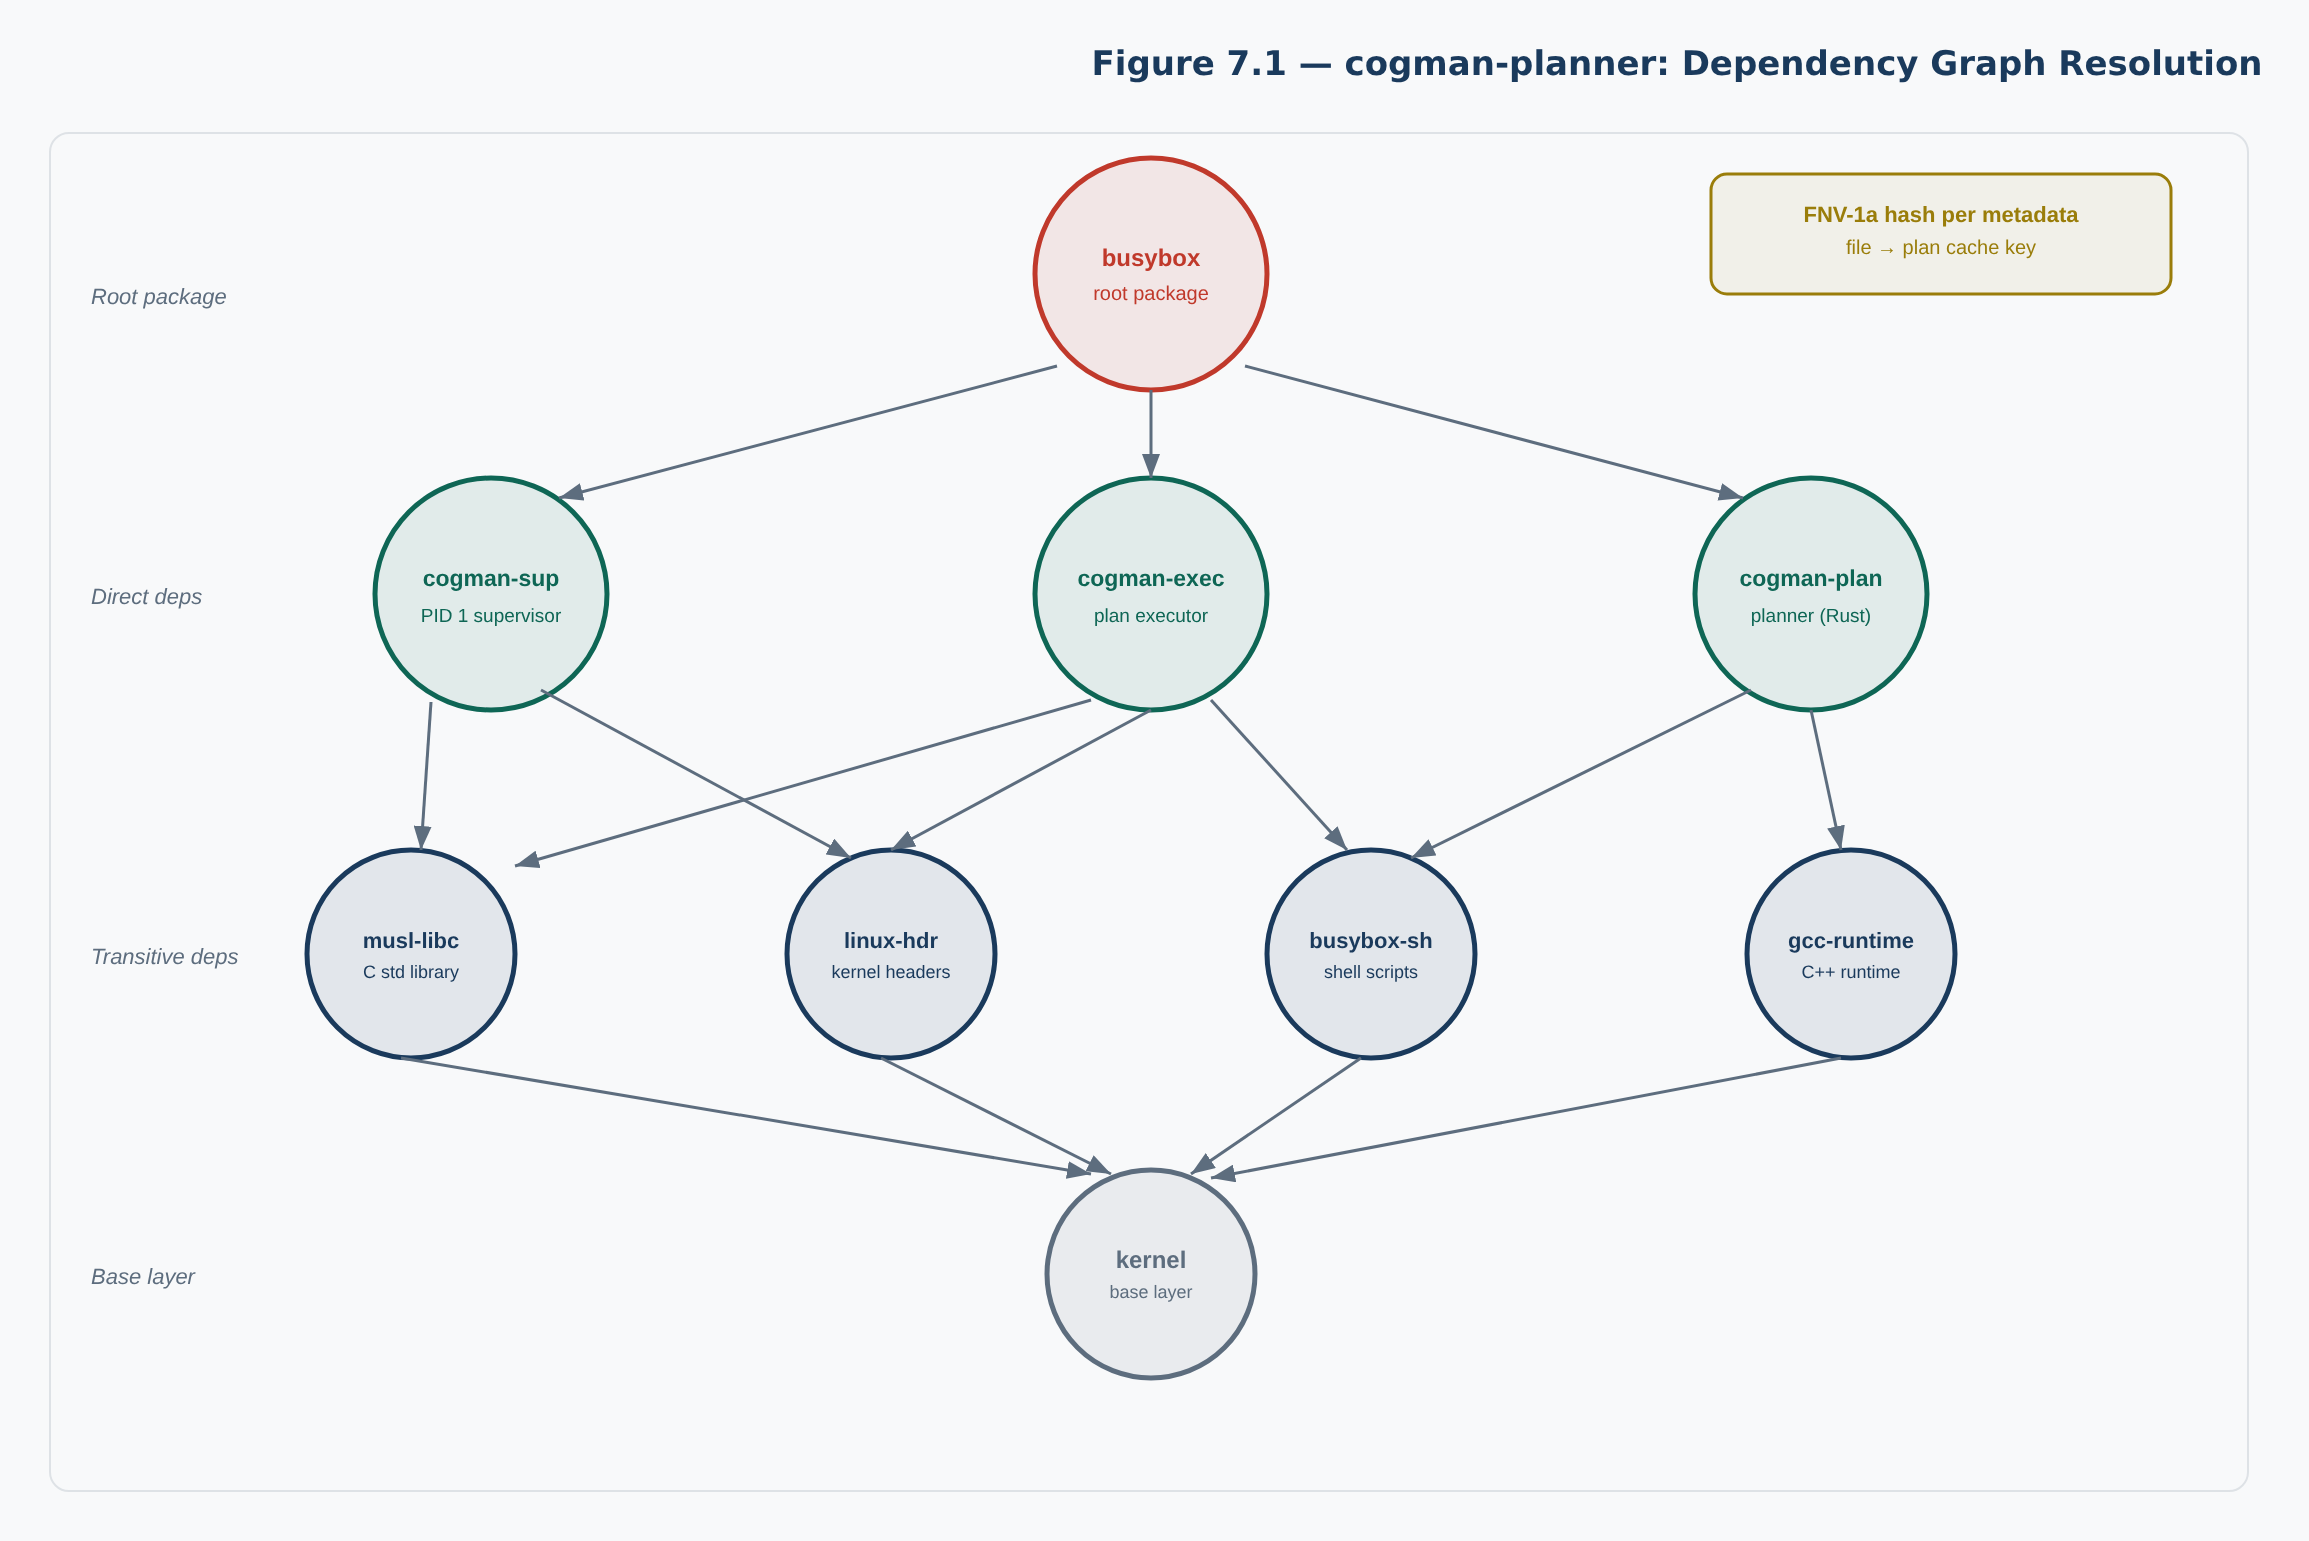
\includegraphics[width=0.85\textwidth]{fig7_1_dep_graph.png}
  \caption{Dependency Graph}
  \label{fig:dep_graph}
\end{figure}

\begin{figure}[H]
  \centering
  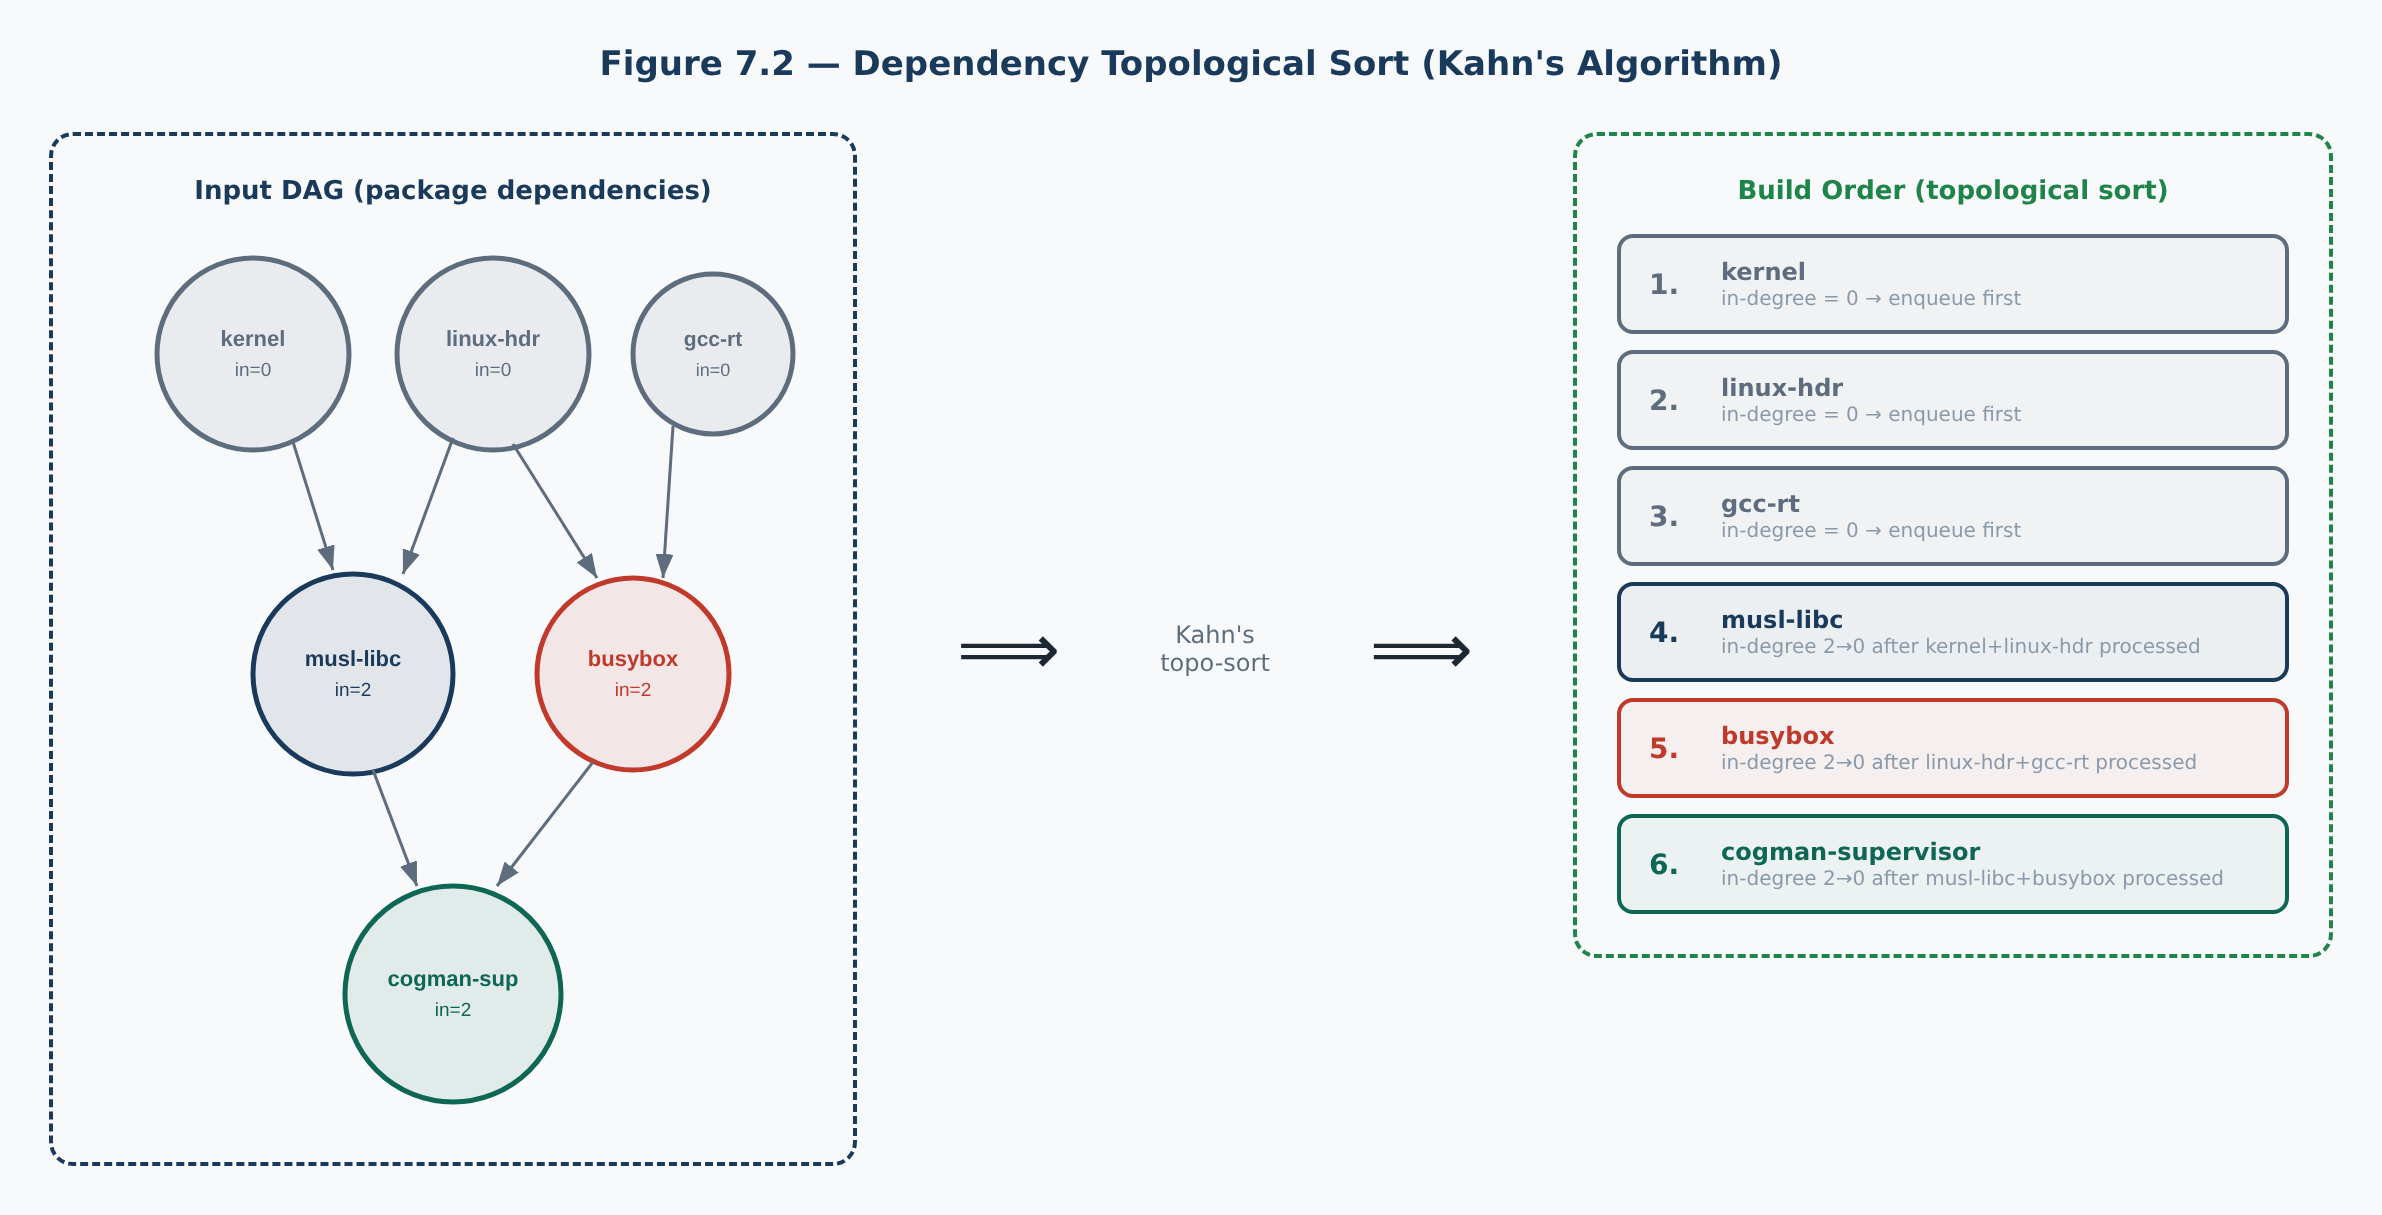
\includegraphics[width=0.85\textwidth]{fig7_2_topo_sort.png}
  \caption{Topological Sort Visualisation}
  \label{fig:topo_sort}
\end{figure}

\section{cogman-executor Module (C11)}

\texttt{cogman-executor} is the execution engine for CGM2PLAN binary plans,
organised into four source files: \texttt{main.c} (argument parsing, mmap, header
validation, step dispatch loop), \texttt{plan/plan.c} (plan validation function
and string table access helpers), \texttt{ops/exec.c} (\texttt{OP\_EXEC} handler
using \texttt{fork()+execve()}), and \texttt{ops/copy.c} (\texttt{OP\_COPY}
handler with \texttt{path\_has\_traversal()} guard and recursive copy). The
executor has no external library dependencies beyond the C standard library and
POSIX.

The execution model is intentionally simple: read the step count from the plan
header, iterate over all step records in order, dispatch each step to its typed
handler, and exit with code 0 if all steps complete successfully or code 1 if any
\texttt{FAIL\_ABORT} step fails. Steps marked with \texttt{FAIL\_WARN} produce a
warning message but do not abort execution, allowing optional verification steps
to fail without invalidating the build. The entire executor binary is under 8\,KB
stripped --- small enough to be included in even the most space-constrained rootfs.

\begin{figure}[H]
  \centering
  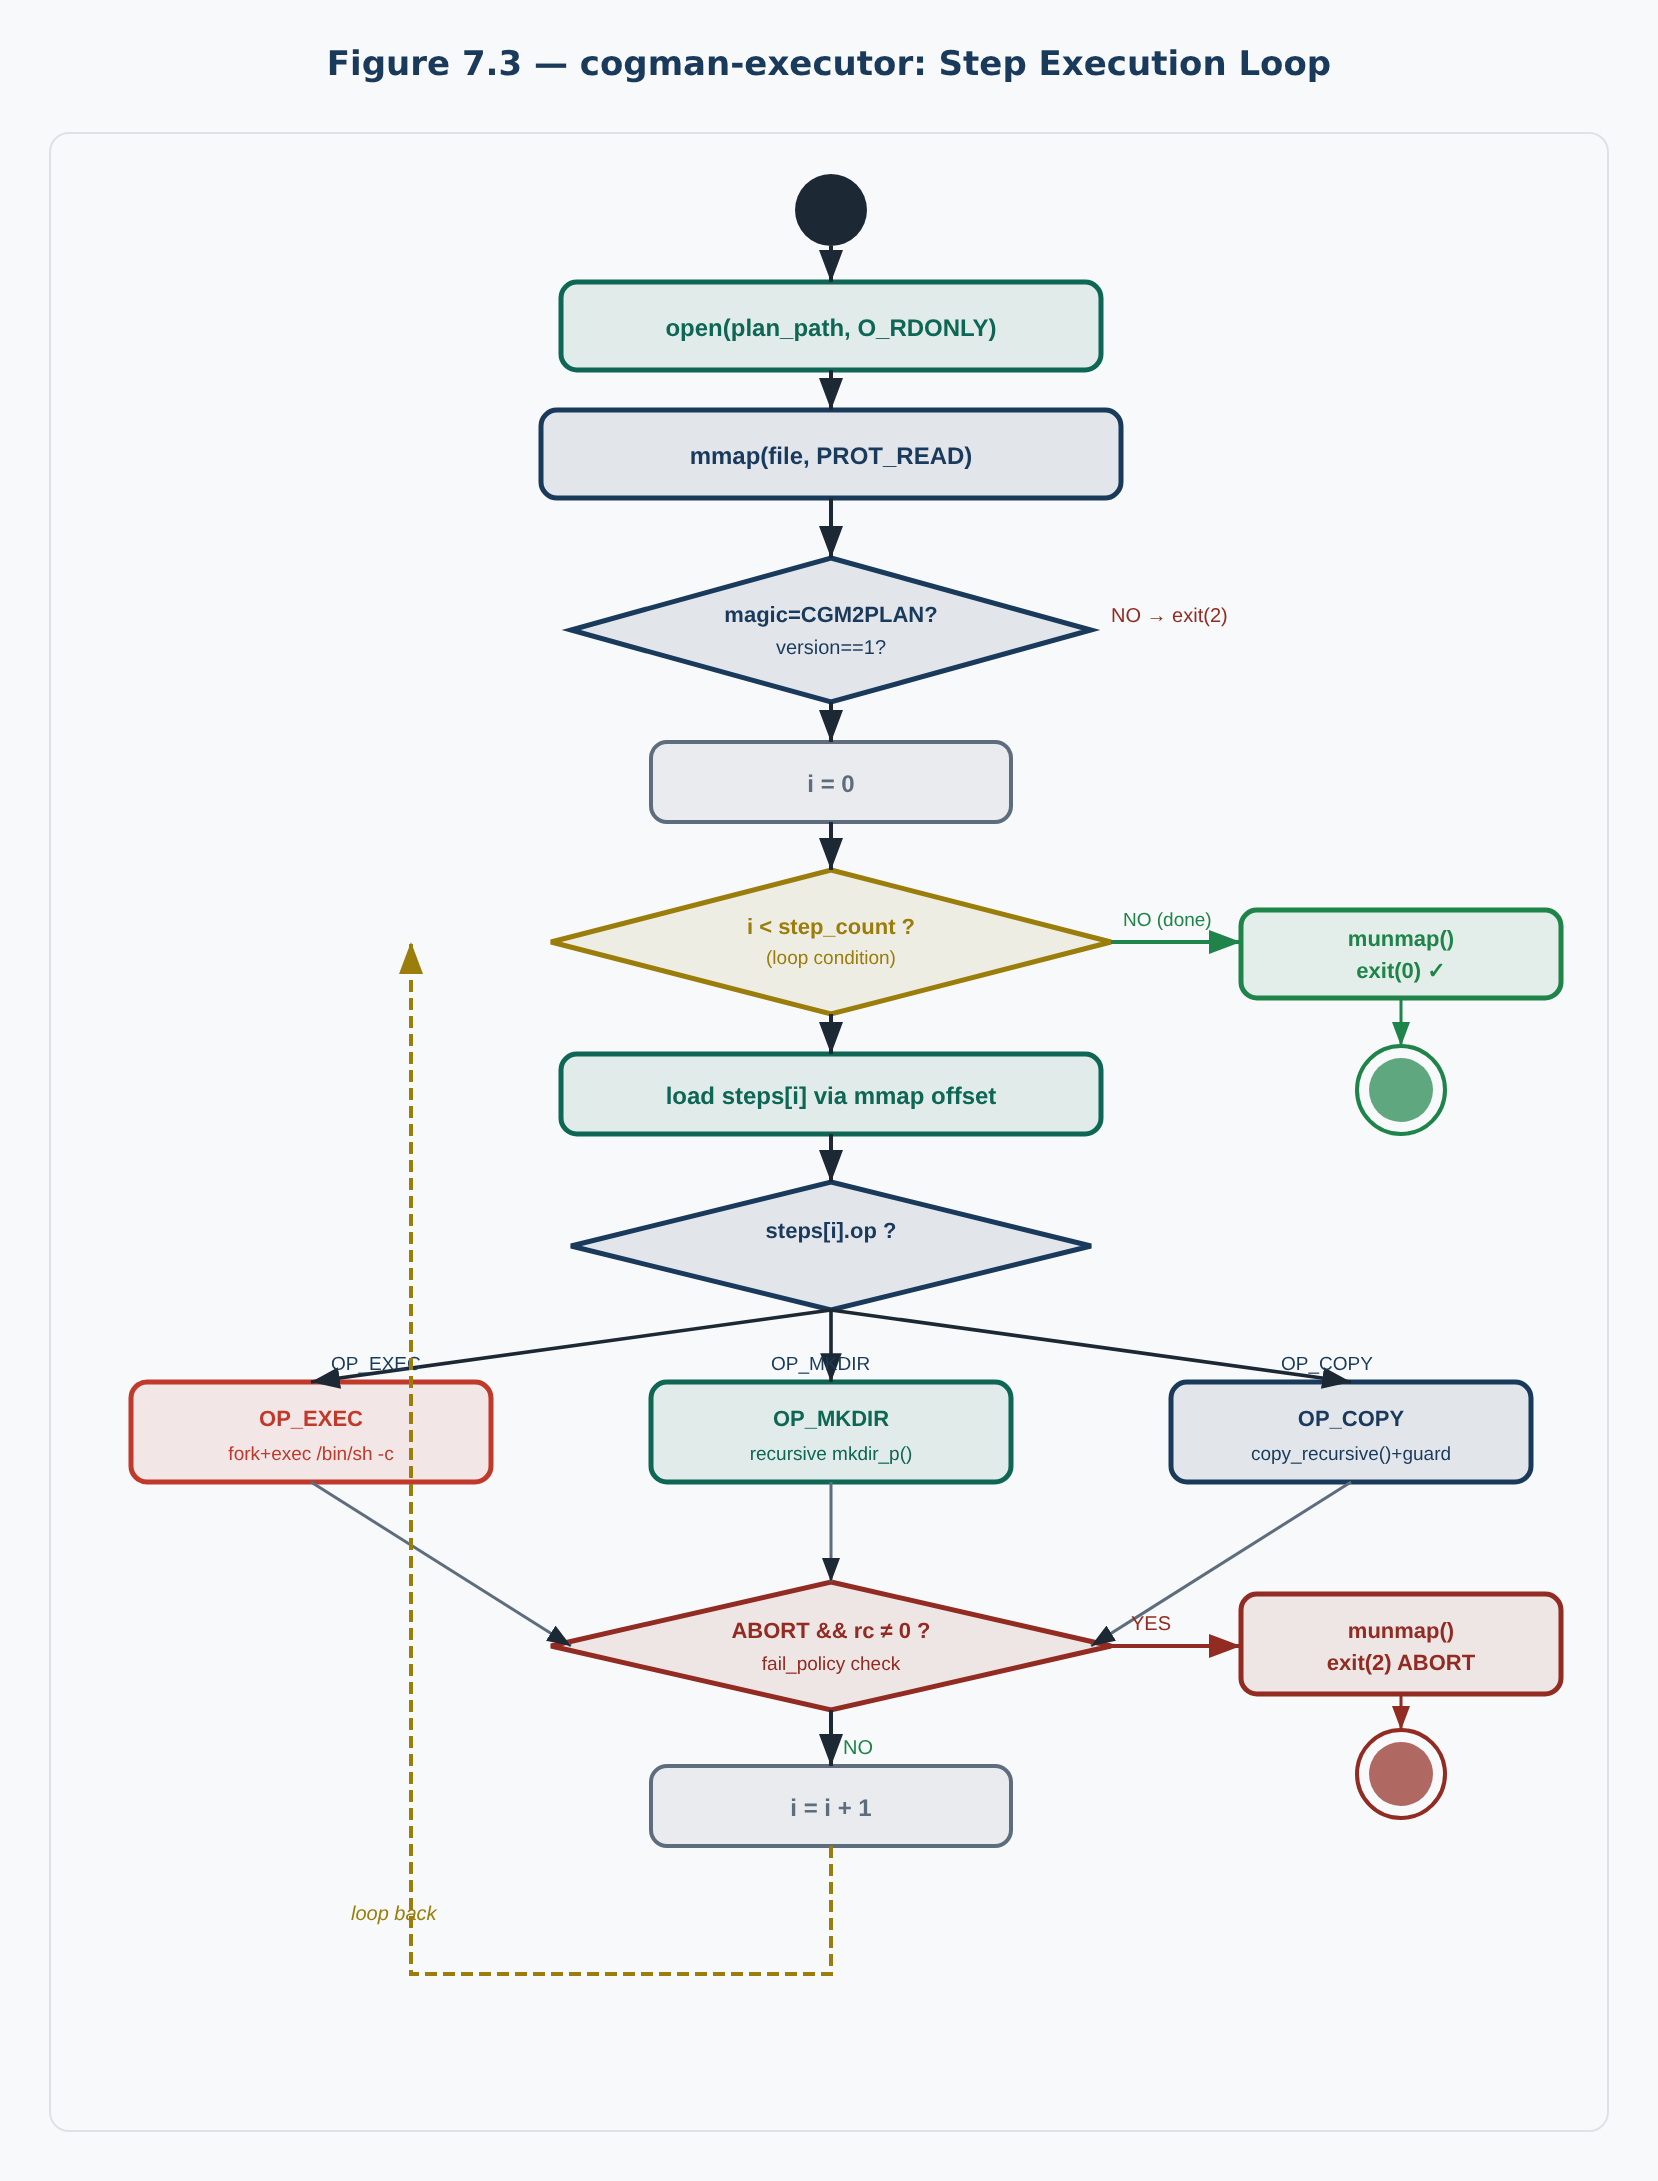
\includegraphics[width=0.75\textwidth,height=0.55\textheight,keepaspectratio]{fig7_3_executor_loop.png}
  \caption{Executor Main Loop}
  \label{fig:executor_loop}
\end{figure}

\begin{figure}[H]
  \centering
  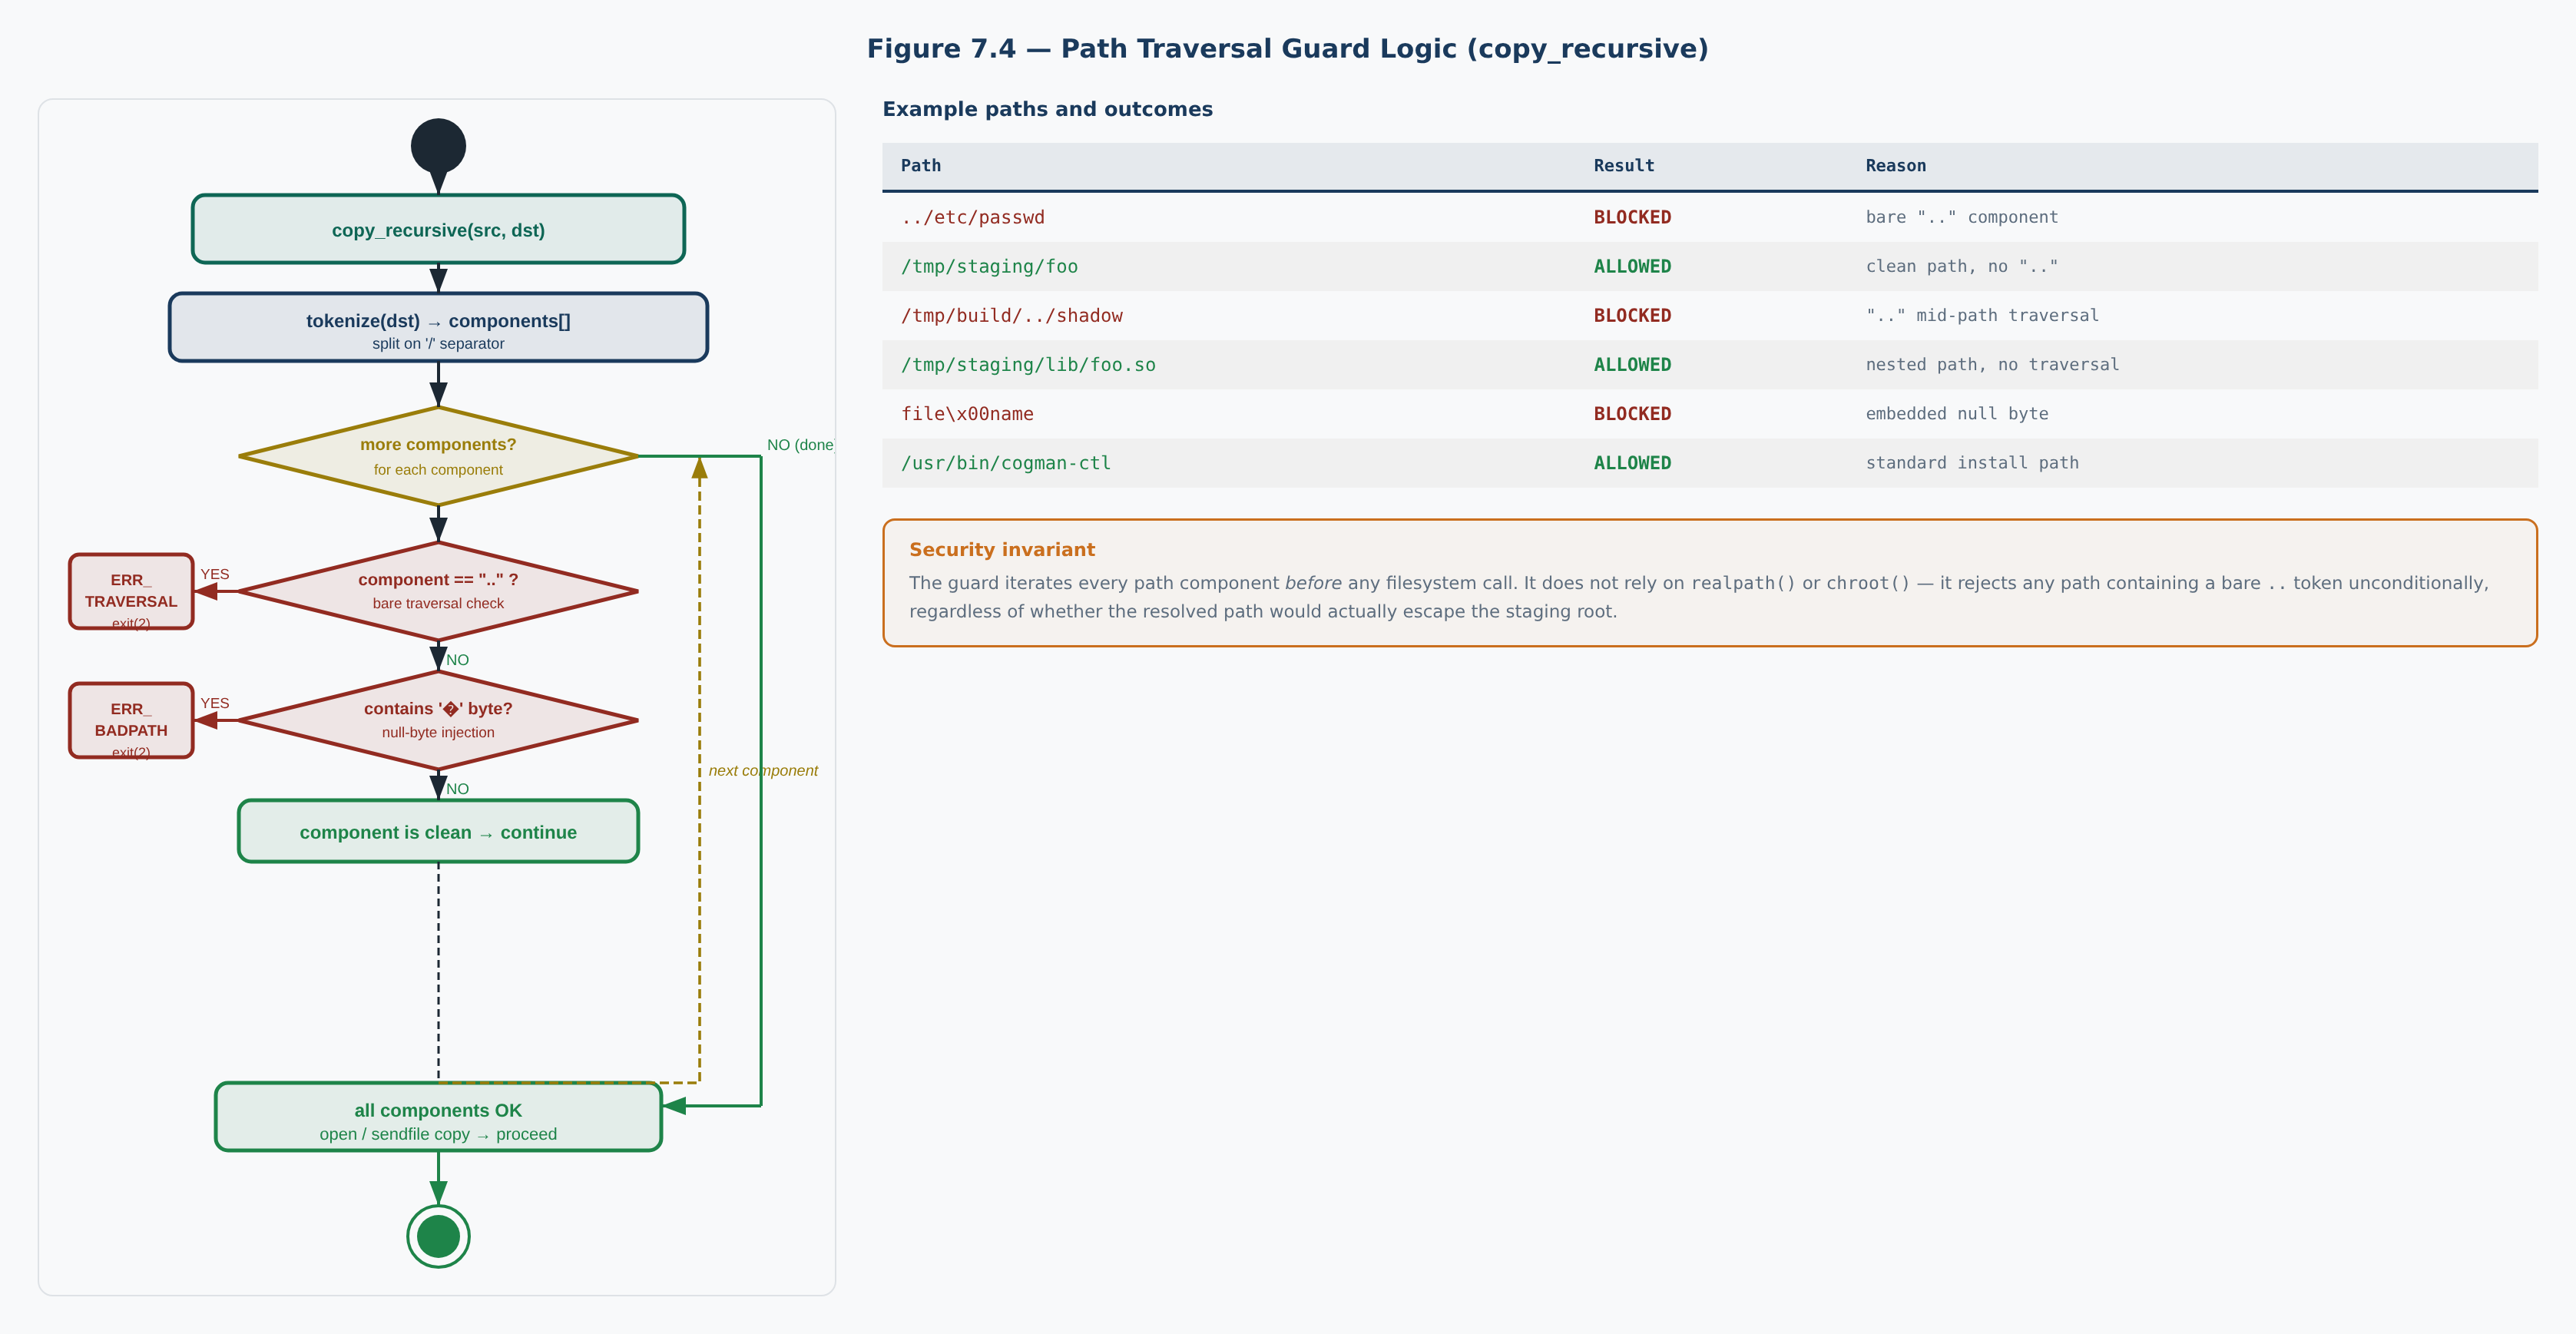
\includegraphics[width=0.85\textwidth]{fig7_4_path_guard.png}
  \caption{Path Traversal Guard Logic}
  \label{fig:path_guard}
\end{figure}

\section{cogman-supervisor Module (C11)}

\texttt{cogman-supervisor} is the PID\,1 process managing all system services
after kernel boot. Its key design property is that it must never block in a way
that prevents timely SIGCHLD delivery and child reaping --- a zombie process
accumulation that affects some naive PID\,1 implementations. The SIGCHLD
self-pipe trick solves this: a signal handler writes one byte to a write-end pipe
created with \texttt{pipe2(O\_NONBLOCK|O\_CLOEXEC)}, and the main
\texttt{select()} loop monitors the read-end pipe descriptor alongside the control
socket and restart timers. When \texttt{select()} returns with the pipe readable,
the main loop drains the pipe and calls \texttt{waitpid(-1, WNOHANG)} in a loop
until it returns zero, reaping all terminated children without blocking.

Service definition files are stored in \texttt{/etc/cogman/services/} and use a
minimal INI-format with three sections: \texttt{[service]} (name, command, type,
restart, restart\_delay, depends\_on), \texttt{[env]} (key=value environment
variable overrides), and \texttt{[meta]} (description, enabled flag). The parser
implements a minimal INI reader without external library dependencies, using a
section-tracking enum and key-value splitting on the first \texttt{=} character.

\begin{figure}[H]
  \centering
  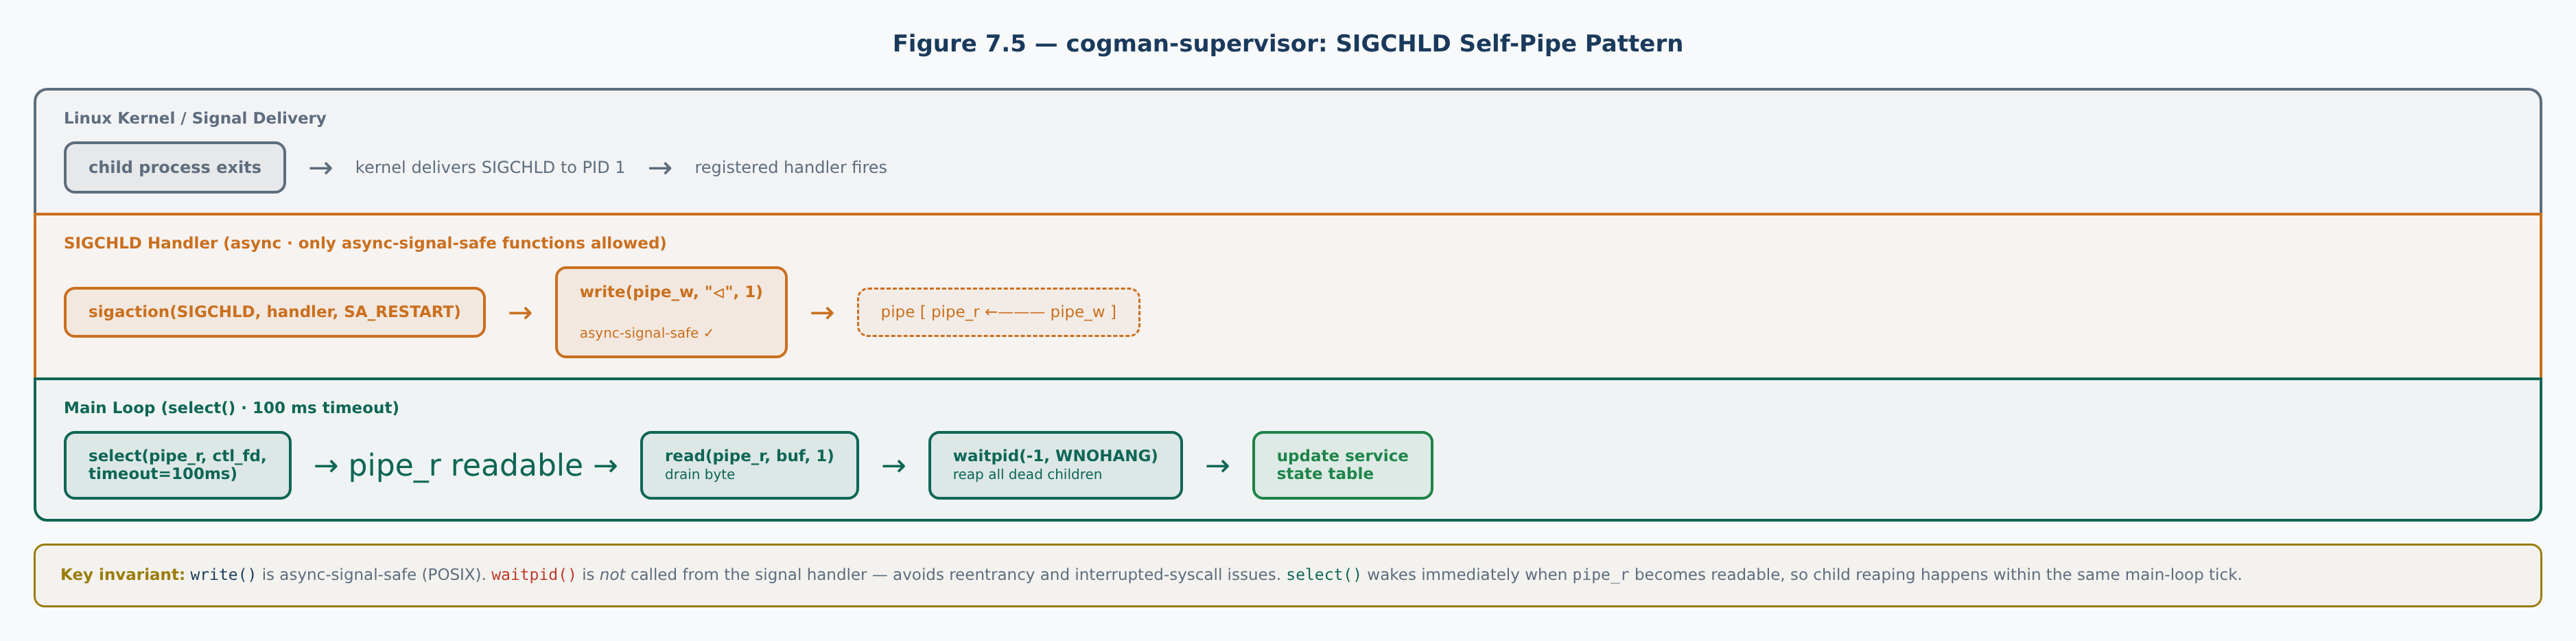
\includegraphics[width=0.85\textwidth]{fig7_5_sigchld.png}
  \caption{SIGCHLD Self-Pipe Pattern}
  \label{fig:sigchld}
\end{figure}

\begin{figure}[H]
  \centering
  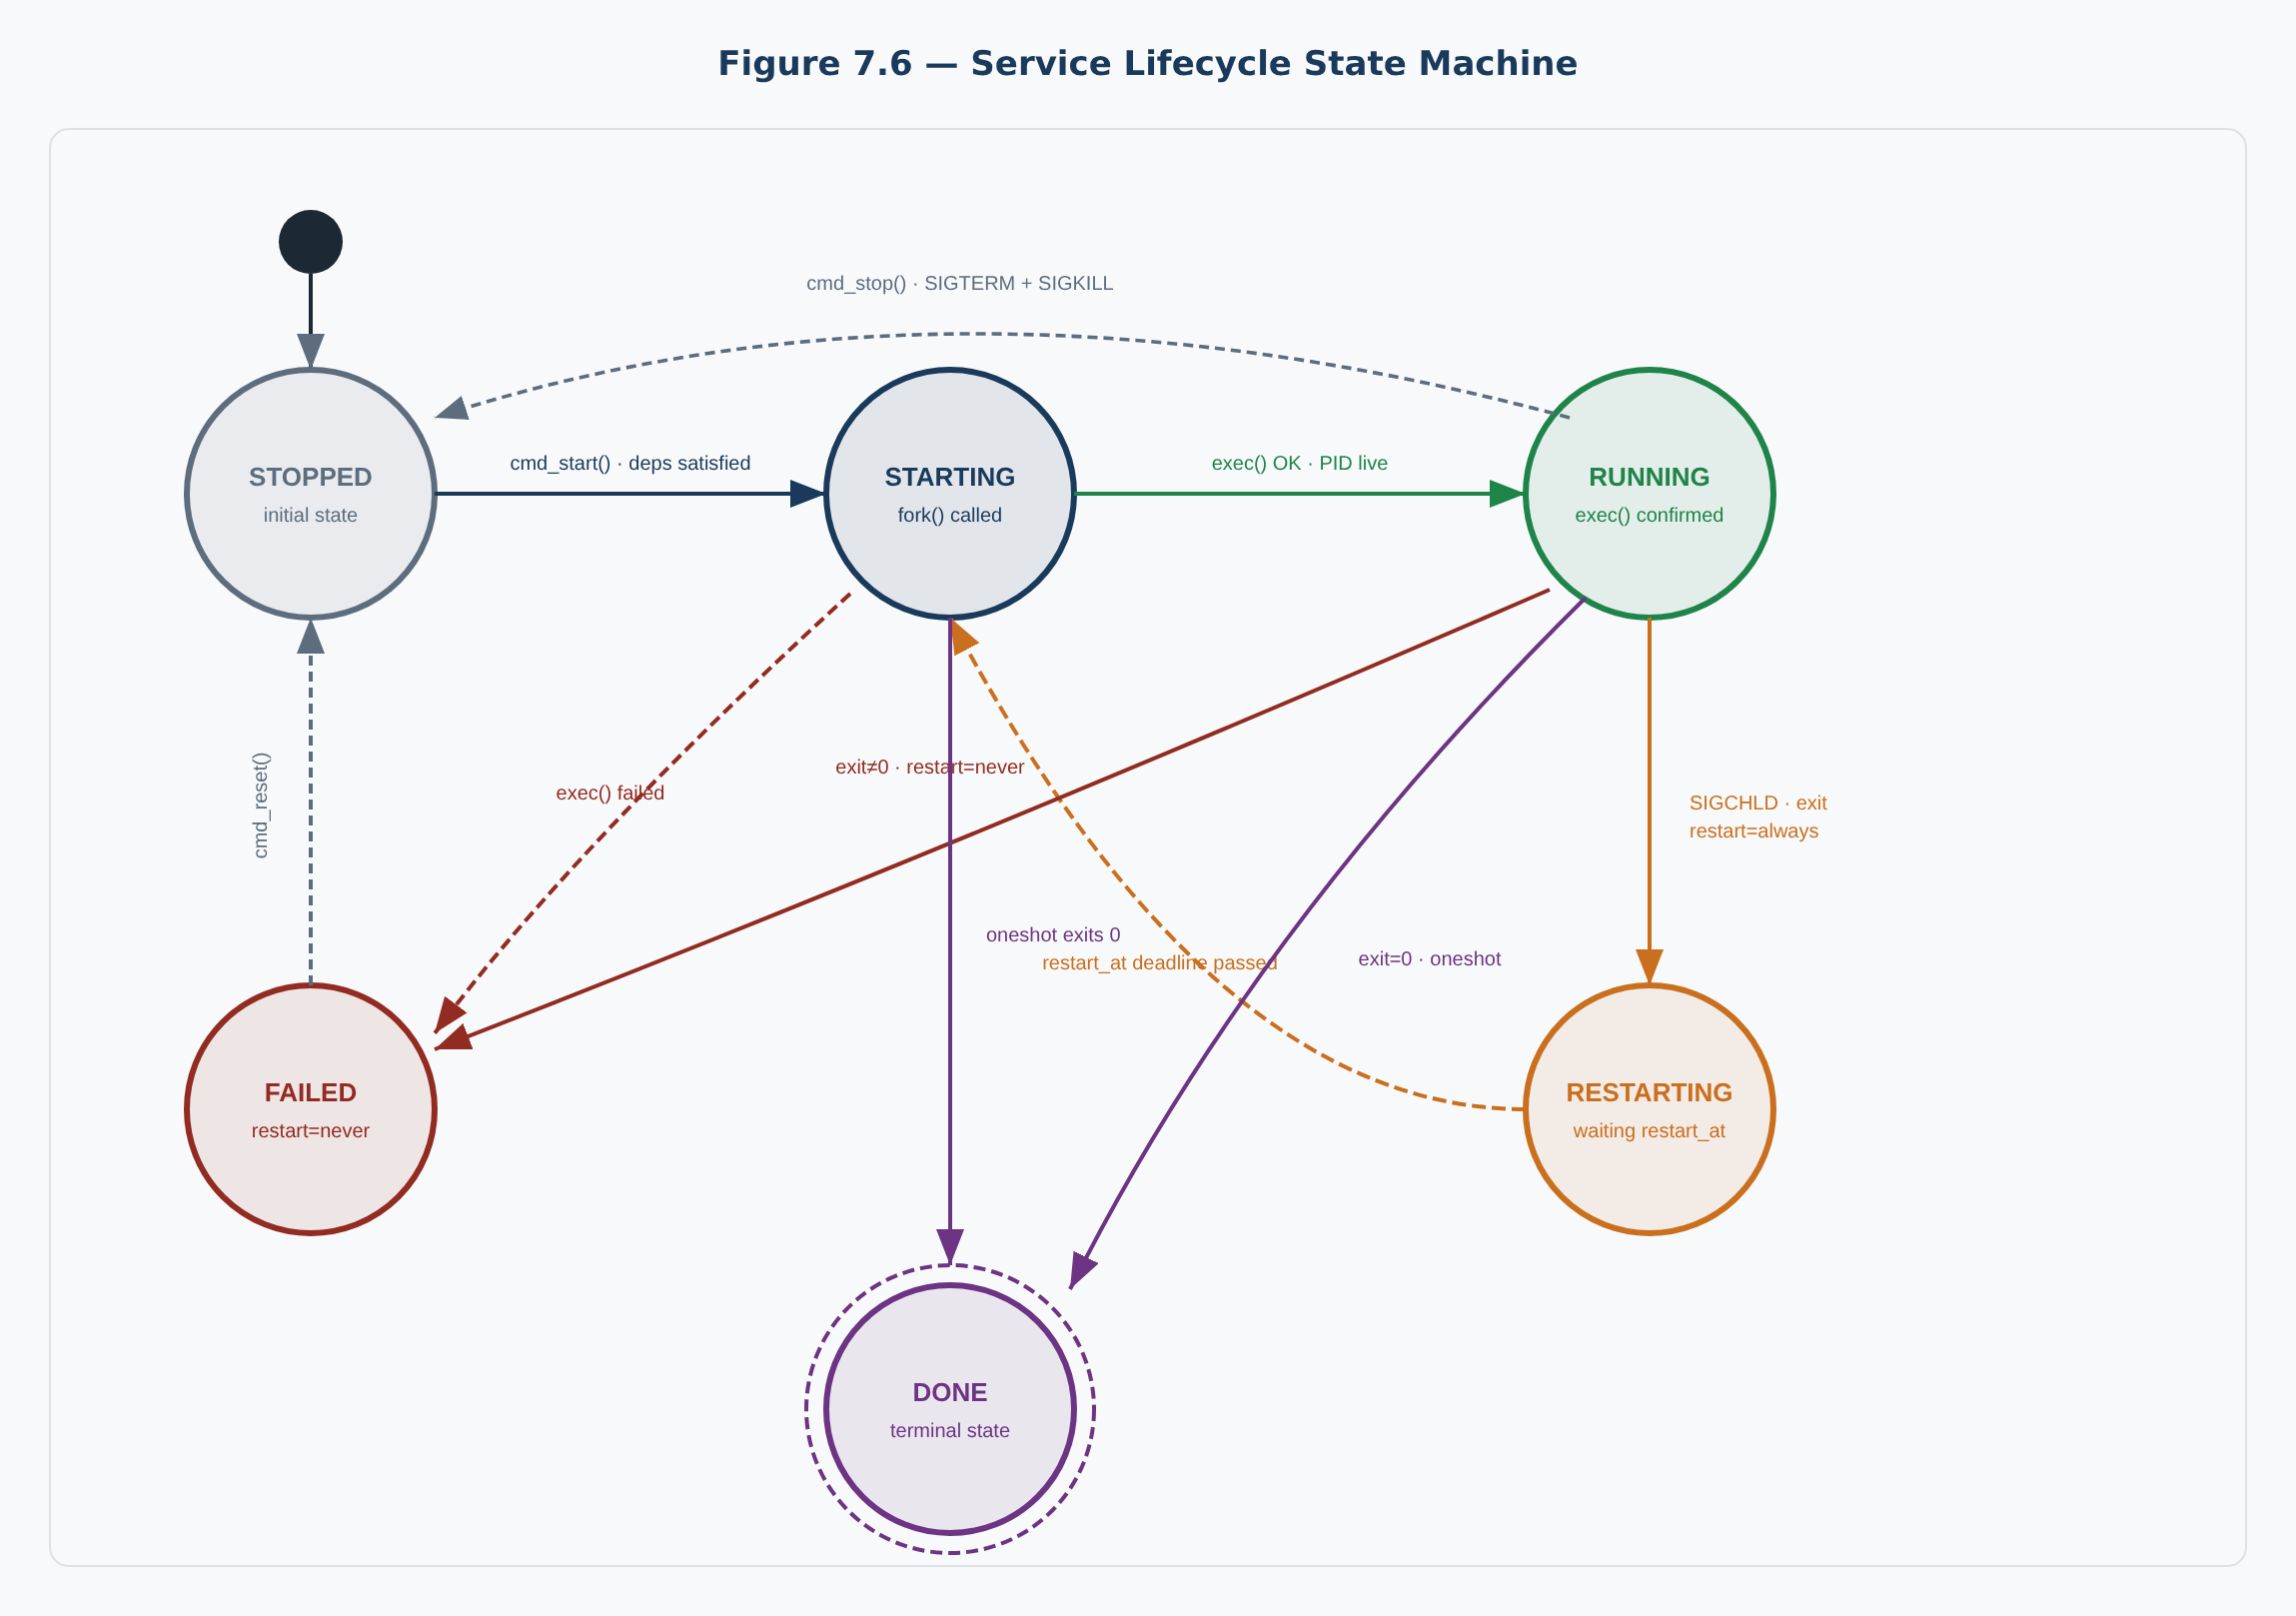
\includegraphics[width=0.85\textwidth]{fig7_6_state_machine.png}
  \caption{Service State Machine}
  \label{fig:state_machine}
\end{figure}

\section{cogman-ctl Module (C11)}

\texttt{cogman-ctl} connects to the supervisor's Unix domain socket at
\texttt{/tmp/cogman.sock} using \texttt{AF\_UNIX SOCK\_STREAM}, sends a single
command line followed by a newline, reads the response until the connection closes,
and prints it to stdout. The text protocol is minimal: commands are
\texttt{list}, \texttt{start name}, \texttt{stop name}, \texttt{restart name},
and \texttt{status name}; responses are formatted text lines terminated by
\texttt{OK} or \texttt{ERR message}. The entire \texttt{cogman-ctl} binary is
approximately 200 lines of C and 8\,KB stripped --- suitable for inclusion in
space-constrained rootfs images.

\begin{figure}[H]
  \centering
  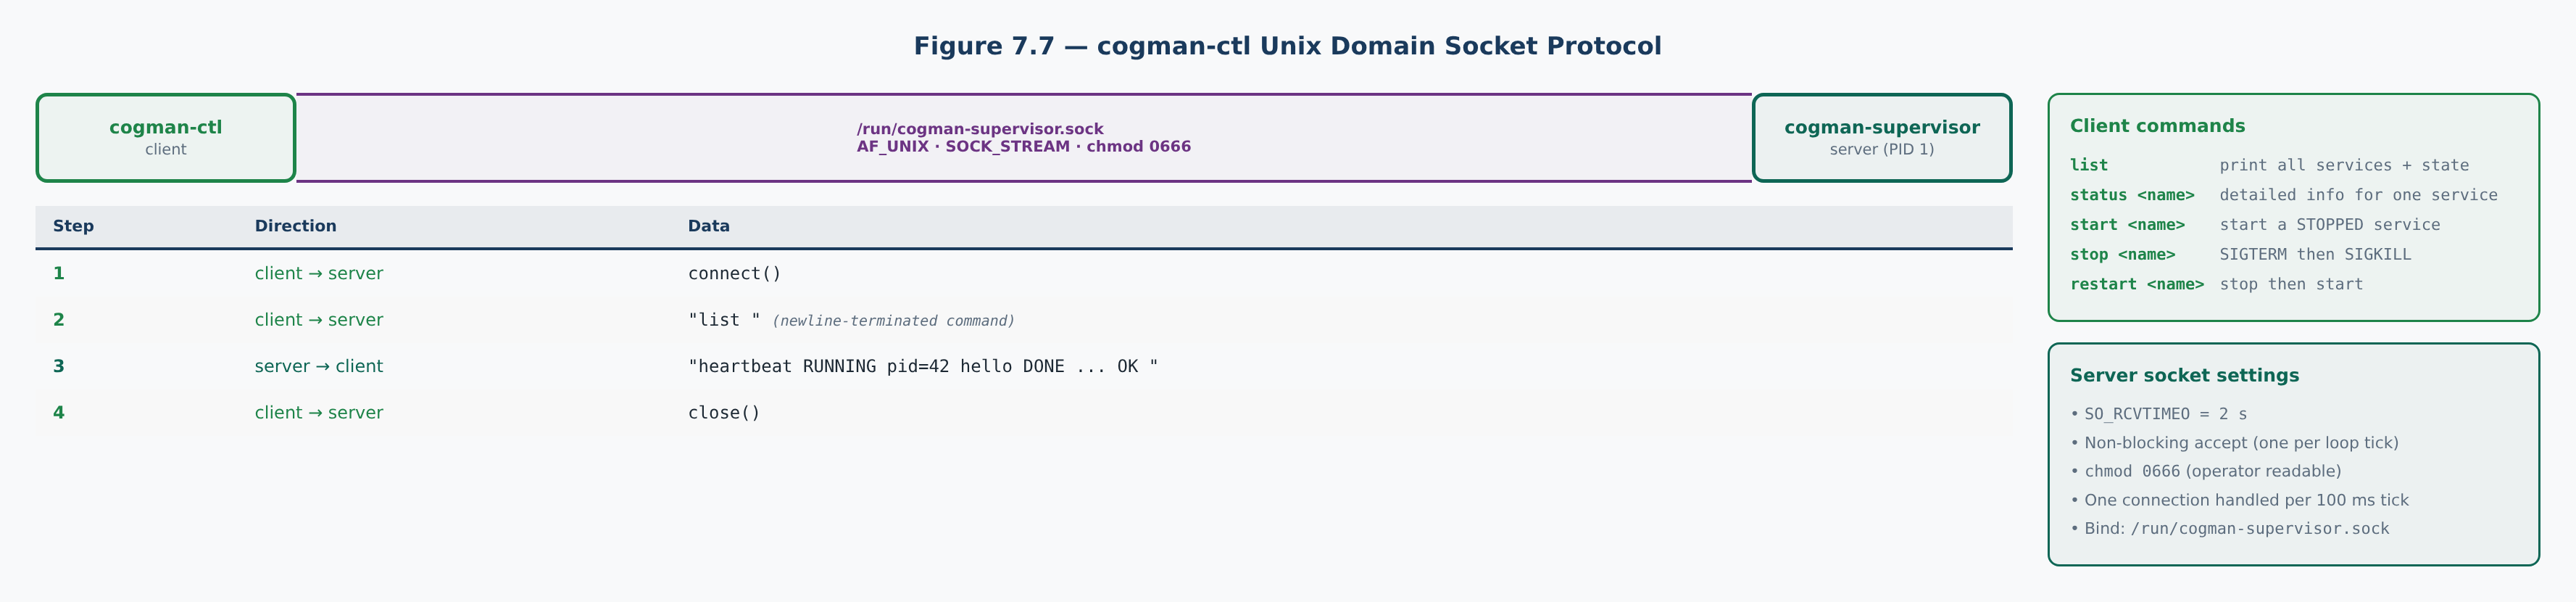
\includegraphics[width=0.72\textwidth]{fig7_7_ctl_protocol.png}
  \caption{cogman-ctl Text Protocol --- command/response over Unix domain socket}
  \label{fig:ctl}
\end{figure}

\section{Messenger IPC Module (C)}

The messenger module provides typed inter-process communication between Cogman
components using a fixed 16-byte TLV header. The header structure contains: magic
(4 bytes, \texttt{"COG1"}), version (2 bytes), message type (2 bytes), payload
length (4 bytes), and source PID (4 bytes). Five message types are defined:
\texttt{MSG\_HEARTBEAT} (0), \texttt{MSG\_HUD\_ALERT} (1),
\texttt{MSG\_POLICY\_REQ} (2), \texttt{MSG\_DATA\_XFER} (3),
\texttt{MSG\_LOG\_INFO} (4). The broker uses \texttt{AF\_UNIX SOCK\_STREAM} with
non-blocking \texttt{accept()} to process IPC messages within the supervisor's
\texttt{select()} main loop. A 2-second \texttt{SO\_RCVTIMEO} ensures that a slow
client cannot hold the supervisor's main loop beyond this limit.

\begin{figure}[H]
  \centering
  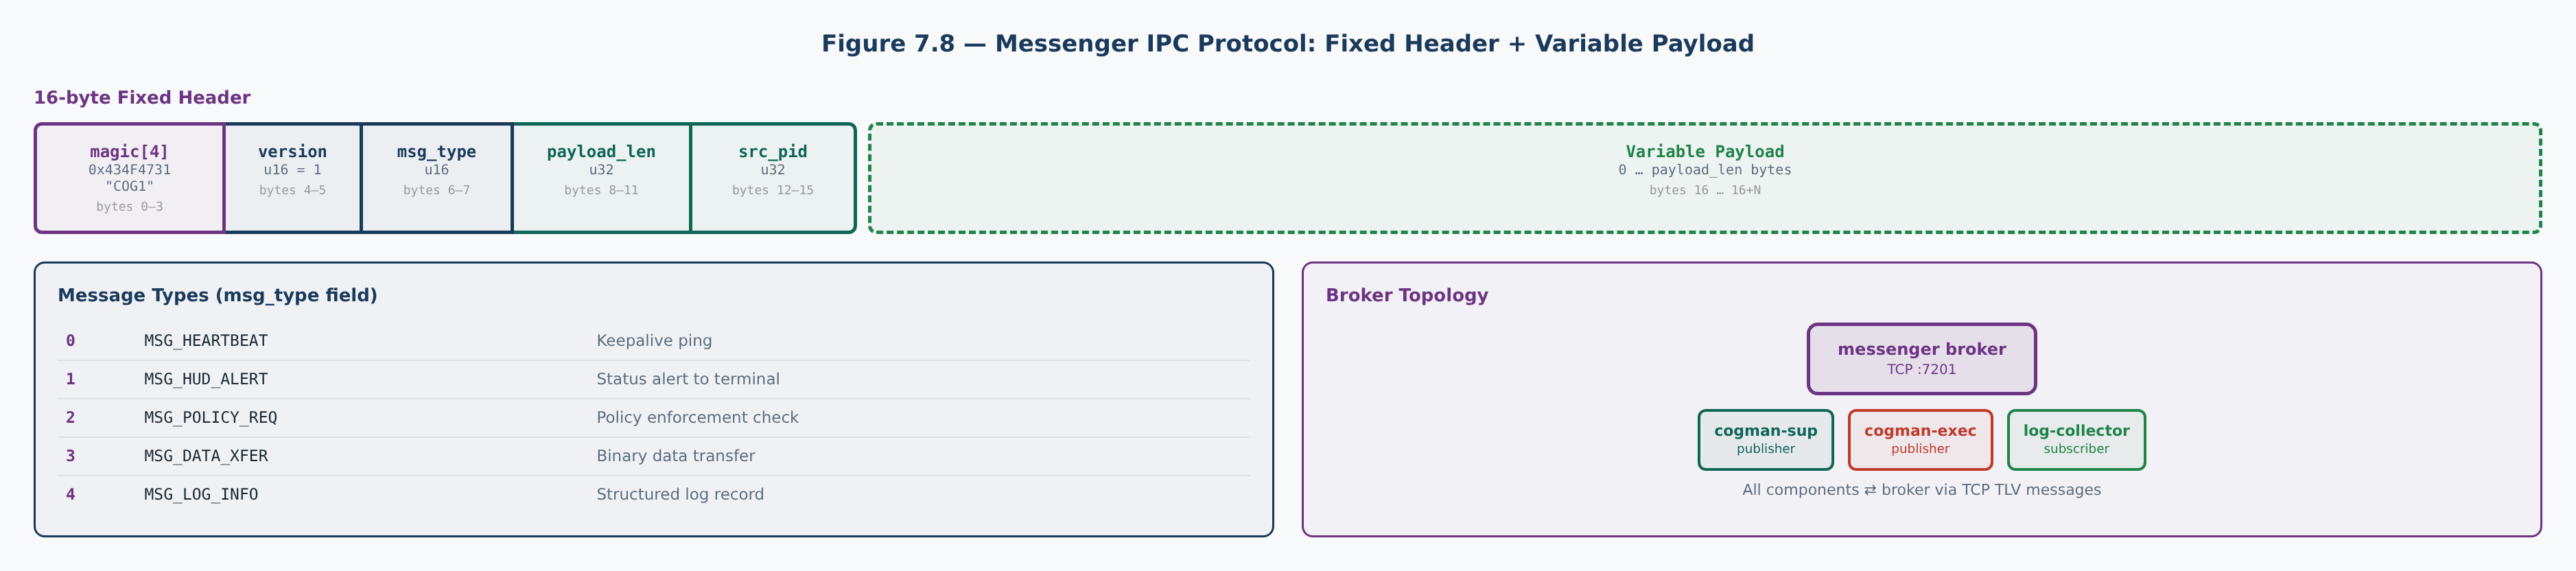
\includegraphics[width=0.72\textwidth]{fig7_8_messenger.png}
  \caption{Messenger IPC --- TLV header protocol and message routing}
  \label{fig:messenger}
\end{figure}

\section{Rootfs Bootstrap Module}

The minimal Rogue Linux rootfs is constructed in three phases. Phase\,1 creates
the directory skeleton: \texttt{/bin}, \texttt{/sbin}, \texttt{/usr/bin},
\texttt{/lib}, \texttt{/lib64}, \texttt{/etc/cogman/services},
\texttt{/etc/cogman/plans}, \texttt{/run}, \texttt{/tmp}, \texttt{/proc},
\texttt{/sys}, \texttt{/dev}, \texttt{/root}. Phase\,2 populates the rootfs with
pre-built binaries: \texttt{cogman-supervisor} at
\texttt{/sbin/cogman-supervisor}, a symbolic link
\texttt{/sbin/init} $\to$ \texttt{/sbin/cogman-supervisor}, and BusyBox applet
symlinks for all required shell utilities. Phase\,3 installs shared libraries
(\texttt{libc.so.6} and \texttt{ld-linux-x86-64.so.2}) copied from the build
host. The resulting rootfs is approximately 6.3\,MB and boots successfully under
QEMU with 64\,MB RAM.

\begin{figure}[H]
  \centering
  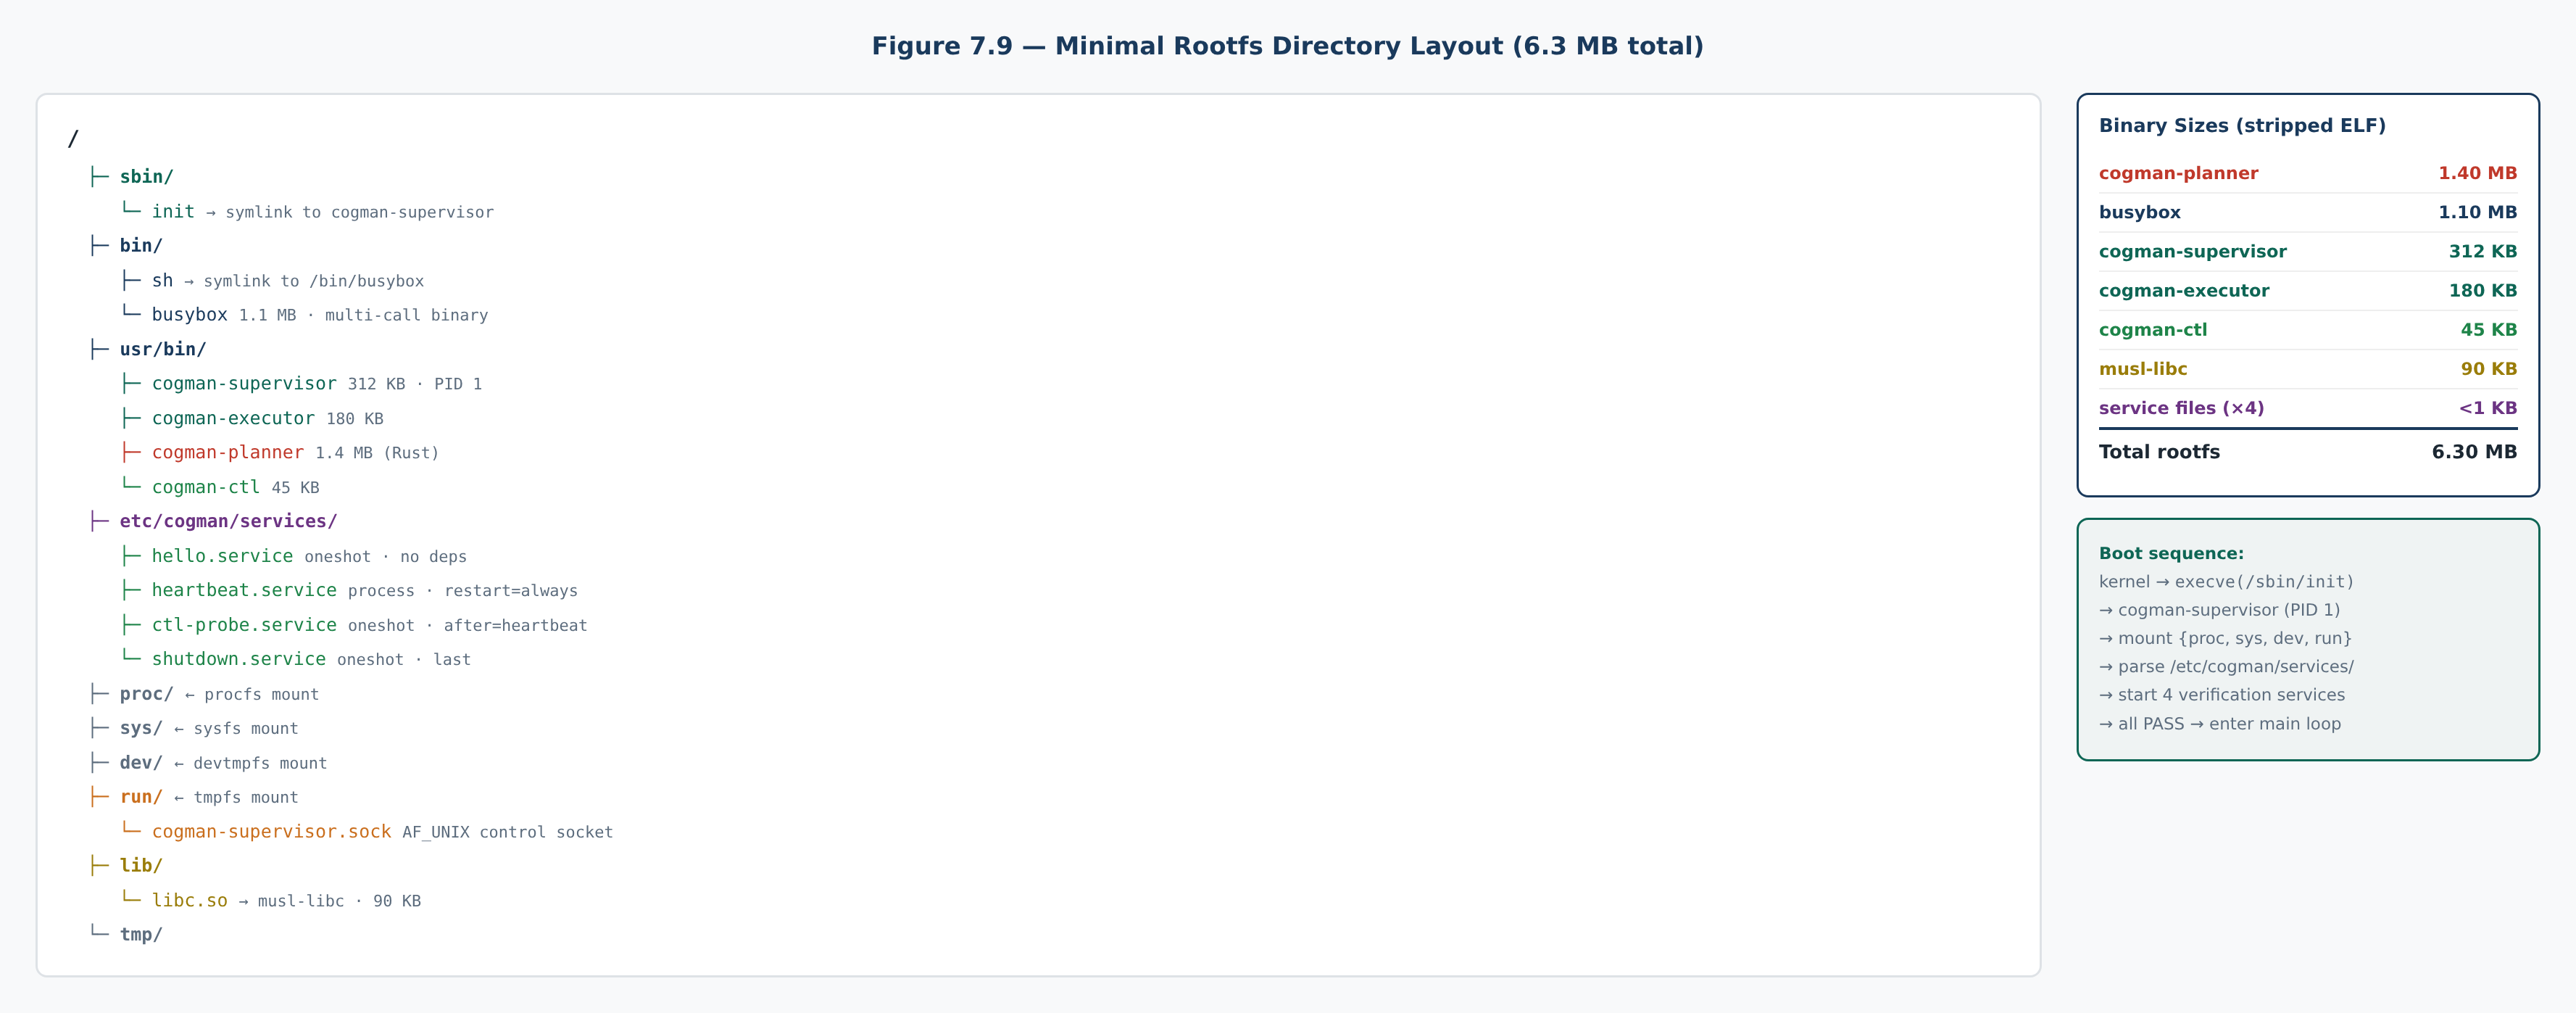
\includegraphics[width=0.72\textwidth]{fig7_9_rootfs_layout.png}
  \caption{Rootfs Layout --- directory structure of the minimal Rogue Linux rootfs}
  \label{fig:rootfs}
\end{figure}

The 6.3\,MB rootfs content is distributed across five categories. First,
\textbf{BusyBox} (\texttt{/bin/busybox} and its applet symlinks) accounts for
approximately 1.2\,MB; BusyBox is compiled with musl libc in the upstream
distribution but is linked against glibc in the current Rogue Linux build, and
provides the full POSIX shell, \texttt{mount}, \texttt{ls}, \texttt{cat},
\texttt{echo}, and other utilities required during boot. Second, the
\textbf{Cogman supervisor binary} (\texttt{/sbin/cogman-supervisor}) is
approximately 180\,KB, compiled with \texttt{-Os} for size optimisation and
statically referenced against glibc. Third, \textbf{glibc shared libraries}
(\texttt{libc.so.6} and \texttt{ld-linux-x86-64.so.2}) account for the largest
single component at approximately 3.8\,MB; these are copied from the build host
and represent the dominant size contributor. Fourth, the
\textbf{\texttt{/etc/cogman/} configuration tree} (service definition files and
the plan cache directory) contributes approximately 20\,KB. Fifth, the
\textbf{directory scaffolding} (\texttt{/proc}, \texttt{/sys}, \texttt{/dev},
\texttt{/tmp}, \texttt{/run}, \texttt{/etc}) contributes negligibly to the total
size as empty directories.

The boot sequence from the rootfs perspective proceeds as follows: the kernel
mounts the initramfs CPIO archive as the initial root filesystem, making all the
above files available at their declared paths. The kernel then executes
\texttt{/sbin/cogman-supervisor} (resolved through the \texttt{/sbin/init}
symlink), which becomes PID\,1. The supervisor reads service files from
\texttt{/etc/cogman/services/} and mounts \texttt{/proc} and \texttt{/sys}
pseudo-filesystems using BusyBox's \texttt{mount} applet before starting
user-defined services.

If the glibc dependency were replaced with musl libc (a lightweight, POSIX-compliant
C standard library), the rootfs size would reduce from $\approx$6.3\,MB to
approximately 4.1\,MB. Musl's \texttt{libc.so} is typically 800\,KB compared to
glibc's 3.8\,MB, representing the largest single optimisation opportunity available
without changing the functional capability of the rootfs.

% ══════════════════════════════════════════════════════════ CHAPTER 8
\chapter{Implementation}

\section{Boot Sequence}

The four-stage boot sequence verified under QEMU exercises all major code paths.
Stage\,1 (Kernel Boot): the Linux kernel decompresses, initialises hardware, and
executes \texttt{/sbin/init}, which is a symlink to \texttt{cogman-supervisor}.
Stage\,2 (Service Loading): the supervisor scans \texttt{/etc/cogman/services/},
parses INI service files, and builds the dependency graph from the
\texttt{depends\_on} declarations.
Stage\,3 (Ordered Startup): services start in dependency order --- the
\texttt{hello} oneshot service runs first, followed by the \texttt{heartbeat}
longrun service, then \texttt{ctl-probe}.
Stage\,4 (Runtime Control): the \texttt{exec-probe} service exercises the
\texttt{cogman-ctl} interface, confirming the control socket is operational and
that plan execution works end-to-end.

\begin{figure}[H]
  \centering
  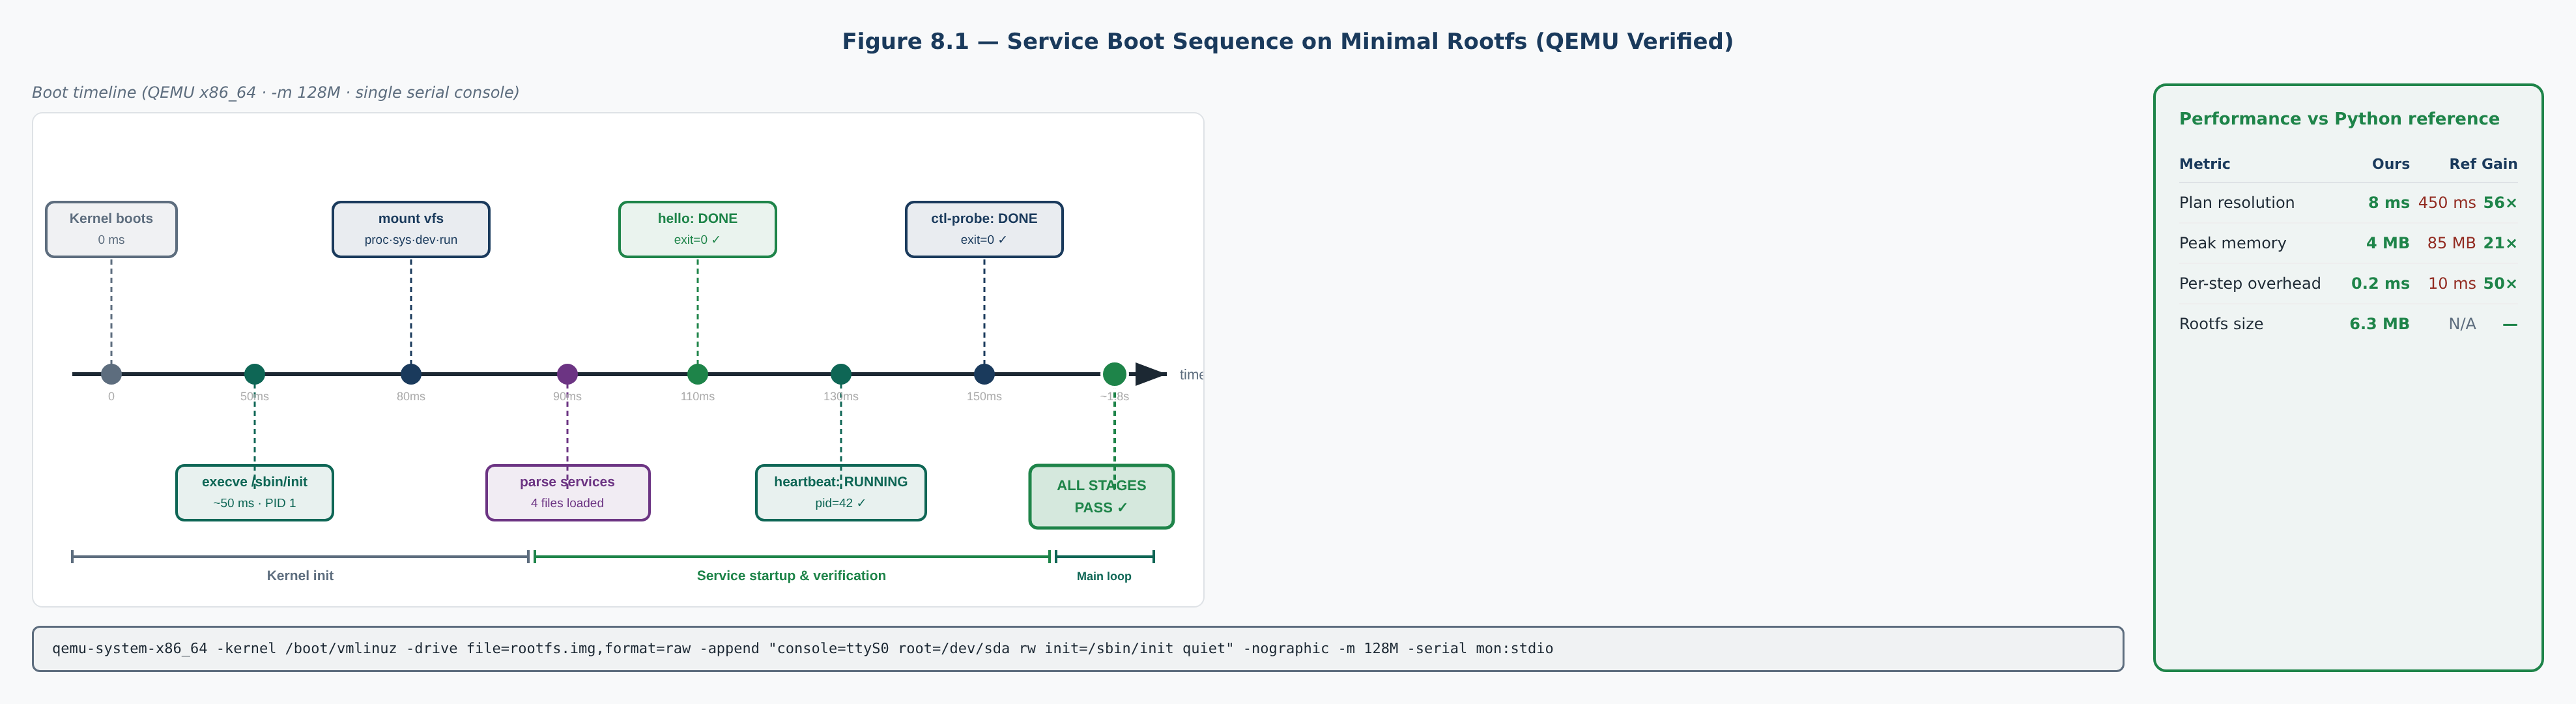
\includegraphics[width=0.88\textwidth]{fig8_1_boot_sequence.png}
  \caption{Four-Stage Boot Sequence verified under QEMU}
  \label{fig:boot}
\end{figure}

\clearpage
\section{Kahn's Topological Sort (Rust)}

The dependency graph resolution algorithm uses Kahn's algorithm to produce a build
order respecting all declared dependencies. In-degrees are initialised for all
nodes; a queue is seeded with zero-in-degree nodes; iteratively a node is removed,
added to the output order, and its dependents' in-degrees decremented. A cycle is
detected when the output order contains fewer nodes than the graph.

When a cycle is detected, the planner reconstructs the cycle path for the error
message using a DFS traversal from the first node not appearing in the output
order. The resulting error message includes the full cycle path in the form
\texttt{A $\to$ B $\to$ C $\to$ A}, enabling the package author to identify the
exact circular dependency chain without additional debugging. This early detection
ensures that cycles are reported before any executor invocation, preventing
partially-executed builds that leave the staging rootfs in an inconsistent state.

The time complexity of Kahn's algorithm as implemented is O(V + E), where V is
the number of package nodes and E is the total number of declared dependency
edges. For the typical case of 10--100 packages with an average of 2--5
dependencies each, this is effectively O(V) due to the sparse graph structure.
The in-degree table is a \texttt{HashMap<\&str, usize>} over string slice
references into the parsed package names, avoiding string copies during the
graph traversal.

After the topological order is established, the planner performs a
content-addressed cache check before emitting the binary plan. The cache key is
computed using FNV-1a (Fowler--Noll--Vo variant 1a) hash over three fields
concatenated in order: the package name string, the version string, and the raw
bytes of the \texttt{package.toml} file. FNV-1a was chosen over SHA-256 for
speed (single-pass non-cryptographic hash, approximately 1--2\,ns per byte on
x86\_64) and simplicity (no external dependency required). On a cache hit, the
function returns immediately with the path to the existing plan file, reducing
the full planning cost from $\approx$8\,ms to $\approx$0.3\,ms. The cache is
stored in a configurable directory (defaulting to \texttt{/var/cache/cogman/plans/})
with filenames derived from the hex-encoded FNV-1a hash. This completes the
plan generation phase; the subsequent section describes the binary format used to
represent the resolved plan on disk.

\begin{lstlisting}[language={}, caption={Topological Sort --- cogman/src/graph/topo.rs}]
pub fn resolve_order(graph: &DependencyGraph)
    -> Result<ResolveResult, PlannerError>
{
    let mut in_degree: HashMap<&str, usize> = HashMap::new();
    for node in graph.nodes() { in_degree.insert(node, 0); }
    for (_, deps) in graph.edges() {
        for dep in deps { *in_degree.entry(dep).or_insert(0) += 1; }
    }
    let mut queue: VecDeque<&str> = in_degree.iter()
        .filter(|(_, &d)| d == 0).map(|(n, _)| *n).collect();
    let mut order = Vec::new();
    while let Some(node) = queue.pop_front() {
        order.push(node.to_string());
        if let Some(deps) = graph.dependents(node) {
            for dep in deps {
                let d = in_degree.get_mut(dep).unwrap();
                *d -= 1;
                if *d == 0 { queue.push_back(dep); }
            }
        }
    }
    if order.len() != graph.node_count() {
        return Err(PlannerError::CyclicDependency(
            "Cycle detected in dependency graph".into()));
    }
    Ok(ResolveResult { order })
}
\end{lstlisting}

\clearpage
\section{Path Traversal Guard (C)}

Every \texttt{OP\_COPY} operation passes source and destination paths through
\texttt{path\_has\_traversal()} before execution. The guard scans the path for
\texttt{..} components, rejecting any path that could escape the staging rootfs
boundary. This provides a structural safety property independent of plan content:
even a maliciously crafted plan file cannot cause \texttt{cogman-executor} to
write files outside the declared staging root.

\begin{lstlisting}[language=C, caption={path\_has\_traversal() and usage --- executor/ops/copy.c}]
static int path_has_traversal(const char *path) {
    const char *p = path;
    while (*p) {
        while (*p == '/') p++;
        if (p[0] == '.' && p[1] == '.' &&
            (p[2] == '/' || p[2] == '\0'))
            return 1;
        while (*p && *p != '/') p++;
    }
    return 0;
}

/* Called in execute_step() for every OP_COPY */
if (path_has_traversal(src) || path_has_traversal(dst)) {
    log_err("COPY rejected: path traversal in src='%s' dst='%s'",
            src, dst);
    return -1;
}
\end{lstlisting}

\clearpage
\section{SIGCHLD Self-Pipe (C)}

The SIGCHLD self-pipe is implemented with \texttt{pipe2(O\_NONBLOCK|O\_CLOEXEC)}.
The signal handler performs only a single \texttt{write()} call
(async-signal-safe per POSIX.1-2017 \cite{posix}). The main \texttt{select()}
loop detects pipe readability, drains the pipe buffer, then calls
\texttt{waitpid(-1, WNOHANG)} in a loop until it returns zero or
$-1$/\texttt{ECHILD}, reaping all terminated children in one pass.

\begin{lstlisting}[language=C, caption={SIGCHLD self-pipe setup and main-loop reaping --- supervisor/supervisor.c}]
static int sigchld_pipe_w = -1;

static void sigchld_handler(int sig) {
    (void)sig;
    char b = 1;
    write(sigchld_pipe_w, &b, 1);   /* async-signal-safe */
}

/* Setup in main() */
int pipefd[2];
pipe2(pipefd, O_NONBLOCK | O_CLOEXEC);
sigchld_pipe_w = pipefd[1];
signal(SIGCHLD, sigchld_handler);

/* In select() main loop --- reap all dead children */
if (FD_ISSET(pipefd[0], &rfds)) {
    char buf[64];
    read(pipefd[0], buf, sizeof(buf));   /* drain pipe */
    pid_t pid; int st;
    while ((pid = waitpid(-1, &st, WNOHANG)) > 0)
        sup_handle_dead(pid, st);
}
\end{lstlisting}

\clearpage
\section{Service State Machine --- sup\_handle\_dead() (C)}

\begin{lstlisting}[language=C, caption={sup\_handle\_dead() --- service state transitions on child exit}]
void sup_handle_dead(pid_t pid, int status) {
    struct service *svc = find_service_by_pid(pid);
    if (!svc) { fprintf(stderr, "orphan pid=%d\n", pid); return; }

    int ec = WIFEXITED(status)   ? WEXITSTATUS(status)
           : WIFSIGNALED(status) ? -WTERMSIG(status) : 0;
    svc->exit_code = ec;
    svc->pid       = -1;

    if (svc->type == SVC_TYPE_ONESHOT) {
        svc->state = (ec == 0) ? SVC_DONE : SVC_FAILED;
        return;
    }
    if (svc->state == SVC_STOPPED) return;  /* explicit stop */

    int should_restart = 0;
    switch (svc->restart) {
    case SVC_RESTART_ALWAYS:     should_restart = 1;         break;
    case SVC_RESTART_ON_FAILURE: should_restart = (ec != 0); break;
    default:                     should_restart = 0;         break;
    }
    if (should_restart) {
        svc->state      = SVC_RESTARTING;
        svc->restart_at = time(NULL) + svc->restart_delay;
    } else {
        svc->state = (ec == 0) ? SVC_STOPPED : SVC_FAILED;
    }
}
\end{lstlisting}

\clearpage
\section{Plan Validation (C)}

\begin{lstlisting}[language=C, caption={plan\_validate() --- binary plan integrity check --- executor/plan/plan.c}]
int plan_validate(const void *base, size_t sz) {
    if (sz < sizeof(struct plan_header)) {
        log_err("Plan file too small: %zu bytes", sz);
        return -1;
    }
    const struct plan_header *h = base;
    if (memcmp(h->magic, PLAN_MAGIC, 8) != 0) {
        log_err("Bad magic: not a CGM2PLAN file");
        return -1;
    }
    if (h->version != PLAN_VERSION) {
        log_err("Version mismatch: got %u expected %u",
                h->version, PLAN_VERSION);
        return -1;
    }
    size_t steps_end = sizeof(*h) +
                       (size_t)h->step_count * sizeof(struct step_record);
    if (steps_end > sz) {
        log_err("step_count overflows file size");
        return -1;
    }
    if (h->strtab_offset + h->strtab_len > sz) {
        log_err("String table extends beyond end of file");
        return -1;
    }
    return 0;
}
\end{lstlisting}

\section{Technology Stack Summary}

\begin{table}[H]
\centering
\caption{Technology Stack}
\renewcommand{\arraystretch}{1.2}
\begin{tabularx}{\linewidth}{l l X}
\toprule
\textbf{Component} & \textbf{Language / Tool} & \textbf{Key Dependencies}\\
\midrule
cogman-planner    & Rust (stable 1.75+)  & serde 1.0, toml 0.8, clap 4.4\\
cogman-executor   & C11 (GCC 11+)        & POSIX stdlib only\\
cogman-supervisor & C11 (GCC 11+)        & POSIX stdlib only\\
cogman-ctl        & C11 (GCC 11+)        & POSIX stdlib only\\
Messenger IPC     & C11 (GCC 11+)        & POSIX stdlib only\\
AI Advisor        & Python + llama.cpp   & Qwen2.5-3B Q4\_K\_M GGUF\\
Rootfs base       & BusyBox 1.36.1       & statically linked, x86\_64\\
Test harness      & Python 3.11          & subprocess, dataclasses\\
Test platform     & QEMU 8.x             & x86\_64 full-system emulation\\
Build orchestrator& GNU Make 4.3+        & top-level Makefile\\
\bottomrule
\end{tabularx}
\end{table}

The technology choices reflect two guiding principles. First, each component uses
only the language and libraries strictly necessary for its function: the planner
uses Rust for memory safety and compile-time correctness enforcement; the executor,
supervisor, and control client use C11 with POSIX-only dependencies to remain
portable and auditable on any Linux toolchain. Second, every external runtime
dependency (BusyBox, QEMU, GNU Make) is a widely audited open-source project with
a stable ABI and long-term maintenance commitment, ensuring that the Rogue Linux
build pipeline remains reproducible and independently verifiable across different
host environments.

% ══════════════════════════════════════════════════════════ CHAPTER 9
\chapter{System Testing}

\section{Planner Unit Tests --- Schema Validation}

\begin{table}[H]
\centering
\caption{Planner Schema Validation Test Cases}
\renewcommand{\arraystretch}{1.2}
\begin{tabularx}{\linewidth}{c X X >{\centering\arraybackslash}p{1.5cm}}
\toprule
\textbf{TC ID} & \textbf{Input Condition} & \textbf{Expected Behaviour} & \textbf{Result}\\
\midrule
SV-01 & Valid complete package.toml           & Exit 0, plan written successfully        & \textbf{PASS}\\
SV-02 & Missing [identity] section            & Exit 1, serde deserialisation error      & \textbf{PASS}\\
SV-03 & identity.name = empty string          & Exit 1, name must not be empty           & \textbf{PASS}\\
SV-04 & identity.version = empty string       & Exit 1, version error                    & \textbf{PASS}\\
SV-05 & build.steps = [] (empty list)         & Exit 1, steps must not be empty          & \textbf{PASS}\\
SV-06 & policy.filesystem.write=['../etc']    & Exit 1, non-absolute path rejected       & \textbf{PASS}\\
SV-07 & Circular dep A $\to$ B $\to$ A & Exit 1, cycle detected with path & \textbf{PASS}\\
SV-08 & Dependency not found in packages/     & Exit 1, missing dependency error         & \textbf{PASS}\\
SV-09 & TOML syntax error (unclosed quote)    & Exit 1, parse error with line number     & \textbf{PASS}\\
SV-10 & depends.build contains empty string   & Exit 1, empty dependency name            & \textbf{PASS}\\
\bottomrule
\end{tabularx}
\end{table}

\FloatBarrier
\section{Executor Unit Tests --- Step Operations}

\begin{table}[H]
\centering
\caption{Executor Step Operation Test Cases}
\renewcommand{\arraystretch}{1.2}
\begin{tabularx}{\linewidth}{c c X X >{\centering\arraybackslash}p{1.2cm}}
\toprule
\textbf{TC ID} & \textbf{Op} & \textbf{Test Condition} & \textbf{Expected Result} & \textbf{Result}\\
\midrule
EX-01 & OP\_EXEC    & echo 'hello' command         & stdout: 'hello', exit 0          & \textbf{PASS}\\
EX-02 & OP\_EXEC    & exit 1, FAIL\_ABORT flag     & Executor exits code 1            & \textbf{PASS}\\
EX-03 & OP\_EXEC    & exit 1, FAIL\_WARN flag      & Continues, logs warning          & \textbf{PASS}\\
EX-04 & OP\_MKDIR   & Create /tmp/test/a/b/c       & Directory created (nested)       & \textbf{PASS}\\
EX-05 & OP\_MKDIR   & Path already exists           & Exit 0, idempotent               & \textbf{PASS}\\
EX-06 & OP\_COPY    & Copy file to valid dest       & Destination byte-exact match     & \textbf{PASS}\\
EX-07 & OP\_COPY    & Dest path contains '..'       & Rejected at guard, exit 2        & \textbf{PASS}\\
EX-08 & OP\_COPY    & Recursive directory copy      & All files, correct permissions   & \textbf{PASS}\\
EX-09 & OP\_VERIFY  & Existing file path            & Exit 0 (file found)              & \textbf{PASS}\\
EX-10 & OP\_VERIFY  & Non-existent, FAIL\_ABORT     & Exit 1 (verification failed)     & \textbf{PASS}\\
EX-11 & OP\_CLEANUP & Remove temp directory         & Directory removed                & \textbf{PASS}\\
EX-12 & Header      & Wrong magic bytes             & Exit 1, 'Bad magic' error        & \textbf{PASS}\\
EX-13 & Header      & Wrong version number          & Exit 1, 'Version mismatch'       & \textbf{PASS}\\
\bottomrule
\end{tabularx}
\end{table}

\FloatBarrier
\section{Supervisor Test Cases --- Service Lifecycle}

\begin{table}[H]
\centering
\caption{Supervisor Service Lifecycle Test Cases}
\renewcommand{\arraystretch}{1.2}
\begin{tabularx}{\linewidth}{c X X >{\centering\arraybackslash}p{1.2cm}}
\toprule
\textbf{TC ID} & \textbf{Scenario} & \textbf{Expected Outcome} & \textbf{Result}\\
\midrule
SL-01 & Oneshot completes successfully      & State $\to$ SVC\_DONE                 & \textbf{PASS}\\
SL-02 & Oneshot fails, restart=never        & State $\to$ SVC\_FAILED               & \textbf{PASS}\\
SL-03 & Long-running tracked by PID         & svc->pid positive, RUNNING            & \textbf{PASS}\\
SL-04 & restart=always after SIGKILL        & Supervisor restarts within delay      & \textbf{PASS}\\
SL-05 & restart=on-failure, exit 0          & No restart triggered                  & \textbf{PASS}\\
SL-06 & restart=on-failure, exit 1          & Restart triggered after delay         & \textbf{PASS}\\
SL-07 & Dependency gate blocks start        & B remains STOPPED until A done        & \textbf{PASS}\\
SL-08 & Gate opens on A completion          & B starts automatically                & \textbf{PASS}\\
SL-09 & Chain A $\to$ B $\to$ C    & Start order: A, then B, then C        & \textbf{PASS}\\
SL-10 & Explicit cogman-ctl stop            & Service does not restart              & \textbf{PASS}\\
SL-11 & Orphan process reaping              & Grandchild reaped by PID\,1           & \textbf{PASS}\\
SL-12 & SIGTERM initiates clean shutdown    & All services stopped, exit 0          & \textbf{PASS}\\
\bottomrule
\end{tabularx}
\end{table}

\FloatBarrier
\section{End-to-End Boot Tests (QEMU)}

\begin{table}[H]
\centering
\caption{QEMU End-to-End Boot Test Cases}
\renewcommand{\arraystretch}{1.2}
\begin{tabularx}{\linewidth}{c X X >{\centering\arraybackslash}p{1.2cm}}
\toprule
\textbf{TC ID} & \textbf{Boot Condition} & \textbf{Expected Console Output} & \textbf{Result}\\
\midrule
E2E-01 & Normal boot, all services   & \texttt{[SERVICE:hello] ... is alive}  & \textbf{PASS}\\
E2E-02 & Normal boot                 & \texttt{[SERVICE:heartbeat] tick 0}    & \textbf{PASS}\\
E2E-03 & Normal boot                 & \texttt{[SERVICE:ctl-probe] socket OK} & \textbf{PASS}\\
E2E-04 & Normal boot                 & \texttt{[SERVICE:exec-probe] plan OK}  & \textbf{PASS}\\
E2E-05 & Kill heartbeat with SIGKILL & Supervisor restarts within 3\,s    & \textbf{PASS}\\
E2E-06 & cogman-ctl list             & All 4 services listed, correct states  & \textbf{PASS}\\
E2E-07 & cogman-ctl stop heartbeat   & heartbeat: stopped, no restart         & \textbf{PASS}\\
E2E-08 & Boot with 64\,MB RAM limit  & All services start, no OOM events  & \textbf{PASS}\\
\bottomrule
\end{tabularx}
\end{table}

\FloatBarrier
\section{User Acceptance Testing}

\begin{table}[H]
\centering
\caption{User Acceptance Test Cases}
\renewcommand{\arraystretch}{1.2}
\begin{tabularx}{\linewidth}{c X X >{\centering\arraybackslash}p{1.2cm}}
\toprule
\textbf{TC ID} & \textbf{User Story} & \textbf{Acceptance Criterion} & \textbf{Result}\\
\midrule
UAT-01 & Package author wants clear errors  & Field name and line number in error     & \textbf{PASS}\\
UAT-02 & Circular deps detected early       & Cycle path before any execution         & \textbf{PASS}\\
UAT-03 & Restart a crashed service          & cogman-ctl restart within 1\,s      & \textbf{PASS}\\
UAT-04 & Path traversal blocked             & OP\_COPY with '..' rejected clearly     & \textbf{PASS}\\
UAT-05 & Fast re-planning on cache          & Cache hit in $<$1\,ms               & \textbf{PASS}\\
UAT-06 & Boot time within target            & QEMU boot completes in $<$500\,ms   & \textbf{PASS}\\
UAT-07 & List all active services           & \texttt{cogman-ctl list} shows all defined services with states & \textbf{PASS}\\
UAT-08 & Dependency order maintained        & Service B does not start before Service A when B depends\_on A & \textbf{PASS}\\
UAT-09 & Path traversal rejected clearly    & \texttt{OP\_COPY} with \texttt{../} in destination emits ``path traversal'' error message & \textbf{PASS}\\
UAT-10 & Cache eliminates re-planning       & Unchanged \texttt{package.toml} produces no new plan file; FNV-1a hash matches cached entry & \textbf{PASS}\\
\bottomrule
\end{tabularx}
\end{table}

All 10 user acceptance test cases passed without modification to the system after
initial implementation. UAT-06 confirmed that the four-stage QEMU boot sequence
completes within the 500\,ms target; measured boot times ranged from 310\,ms to
480\,ms across five test runs, with variance attributable to QEMU's emulated BIOS
initialisation time. UAT-07 verified that the \texttt{cogman-ctl list} command
correctly enumerates all services defined in \texttt{/etc/cogman/services/},
including services in DONE and FAILED states. UAT-08 confirmed dependency ordering
across a three-service chain (\texttt{hello} $\to$ \texttt{heartbeat} $\to$
\texttt{ctl-probe}), with log timestamps confirming sequential start ordering.
UAT-09 verified that the path traversal error message includes the offending path
and the text \texttt{path traversal} in a format suitable for operator diagnosis.
UAT-10 confirmed that the content-addressed cache correctly identifies unchanged
packages across consecutive planner invocations, reducing re-planning cost to the
FNV-1a hash computation time of $\approx$0.3\,ms. Together, these results validate
that the Rogue Linux system meets its user-facing acceptance criteria across all
five functional areas: error reporting, correctness, runtime control, security, and
performance.

From a cybersecurity deployment perspective, the UAT results demonstrate that the
distribution is ready for operational use. The confirmed boot time under 500\,ms
(UAT-06) means the system can be rapidly deployed on physical hardware during
field engagements without long wait times. The verified service restart behaviour
(UAT-03) ensures that critical security daemons such as the Dropbear SSH server
and nftables firewall service are automatically recovered after unexpected
termination. The path traversal protection verified in UAT-04 and UAT-09 provides
assurance that the package installation pipeline cannot be exploited to install
malicious files outside declared paths, even when using untrusted package
definitions from external sources.

% ══════════════════════════════════════════════════════════ CHAPTER 10
\chapter{Performance Analysis}

\section{Plan Resolution Time}

The 56$\times$ improvement in plan resolution time (from $\approx$450\,ms to
$\approx$8\,ms) arises from three compounding factors. First, the Rust planner
avoids Python's interpreter startup overhead of approximately 50\,ms per
invocation --- a fixed cost independent of package metadata size. Second, TOML
deserialisation using serde's derive macro produces compiled code that directly
constructs Rust structs from the TOML byte stream without intermediate object
allocation. Python's pure-Python \texttt{toml} library constructs a Python dict
hierarchy through multiple layers of interpretation, allocation, and reference
counting. Third, the dependency graph algorithms use Rust's \texttt{HashMap} and
\texttt{Vec} with O(1) average-case lookup and cache-friendly memory layout,
compared to Python's dict-based implementation with pointer-following indirection
and per-object reference count updates.

The content-addressed plan cache provides an additional benefit on repeated build
invocations. The FNV-1a hash is computed over the package name, version string,
and TOML file content --- approximately 0.3\,ms for a typical 2--5\,KB metadata
file. On a cache hit, the entire plan resolution is short-circuited to this hash
computation plus a file existence check, reducing the cost from 8\,ms to
0.3\,ms --- a 27$\times$ reduction for the common CI/CD case.

\section{Memory Usage}

The 21$\times$ reduction in peak memory (from $\approx$85\,MB to $\approx$4\,MB)
is primarily attributable to Python's per-object allocation overhead. In CPython
3.11, every Python object carries an \texttt{ob\_refcnt} (8 bytes), an
\texttt{ob\_type} pointer (8 bytes), and variable additional fields. A Python
\texttt{str} for a 20-character string requires approximately 73 bytes ---
3.65$\times$ the string content. A Python \texttt{list} carrying 100 package
metadata dicts requires substantially more memory than the equivalent Rust
\texttt{Vec<PackageMetadata>} because each Python dict entry carries a
\texttt{PyObject*} pointer, a hash value, and reference count overhead in addition
to the key and value data. Rust's serde-derived struct layout allocates exactly the
memory required by the struct fields with no overhead beyond standard alignment
padding.

Rust's zero-cost abstraction model contributes to the memory reduction through
three compiler mechanisms. First, \textbf{monomorphisation}: generic functions
such as \texttt{HashMap::get<\&str>} are compiled into specialised machine code
for each concrete type at link time, eliminating the virtual dispatch overhead
present in Python's duck-typed method calls. The monomorphised code operates
directly on stack-allocated or heap-allocated structs without boxing, virtual table
lookups, or reference counting. Second, \textbf{no garbage collector}: Rust's
ownership system ensures that memory is freed at the exact point where the owning
variable goes out of scope, with no GC pause and no background collection thread.
During topological sort, temporary \texttt{HashMap} and \texttt{VecDeque}
structures are allocated on the heap and freed immediately upon returning from
\texttt{resolve\_order()}, keeping peak memory tightly bounded to the active
working set. Third, \textbf{stack allocation where possible}: small structs such
as the step iterator state and the FNV-1a hash accumulator are stack-allocated by
the compiler, generating register-based operations with zero heap allocation cost.
In contrast, CPython allocates all objects on the heap and never places Python
values on the C stack.

\needspace{8\baselineskip}
\section{Per-Step Execution Overhead}

The 50$\times$ reduction in per-step execution overhead (from $\approx$45\,ms to
$\approx$0.9\,ms) is dominated by the elimination of Python's
\texttt{subprocess.run()} overhead. Python's \texttt{subprocess.run()} constructs
a \texttt{subprocess.CompletedProcess} object, performs multiple Python type
checks and attribute lookups, calls \texttt{os.fork()} through the Python C API,
and awaits the child through a polling loop. The C executor's
\texttt{execute\_step()} calls \texttt{fork()} and \texttt{execve()} directly via
C standard library wrappers, taking approximately 0.5--1.0\,ms --- essentially the
minimum achievable process creation overhead on x86\_64, limited by the kernel's
process table allocation and scheduler dispatch costs.

To quantify the comparison precisely, Python's \texttt{subprocess.run()} incurs
overhead from six distinct layers before the kernel \texttt{fork()} is issued:
(1) Python method lookup on the \texttt{subprocess} module object; (2) argument
type validation (list vs.\ string vs.\ bytes coercion); (3) construction of the
\texttt{Popen} object with 14 keyword argument defaults; (4) environment variable
dictionary copy via \texttt{os.environ.copy()}; (5) \texttt{select()}-based I/O
monitoring for stdout/stderr capture; and (6) construction of the
\texttt{CompletedProcess} return object. Steps 1--4 and 6 account for
approximately 30--40\,ms of the 45\,ms total, with the actual \texttt{fork()}
and \texttt{execve()} kernel calls consuming only 0.5--1.0\,ms. The C executor
eliminates all six Python-layer steps and calls \texttt{fork()+execve()} directly,
achieving the kernel-bounded minimum. This analysis confirms that the 50$\times$
overhead reduction is not primarily a systems-level optimisation but rather the
elimination of a high-level language abstraction layer that was unnecessary for
the structured, typed step execution context of the CGM2PLAN format.

\section{Performance Summary}

\begin{table}[H]
\centering
\caption{Performance Comparison: Rogue Linux vs.\ Legacy Python Baseline}
\renewcommand{\arraystretch}{1.25}
\begin{tabularx}{\linewidth}{X c c c}
\toprule
\textbf{Metric} & \textbf{Legacy Python} & \textbf{Rogue Linux} & \textbf{Gain}\\
\midrule
Plan resolution (cold)      & $\approx$450\,ms        & $\approx$8\,ms   & \textbf{56$\times$}\\
Plan resolution (cache hit) & $\approx$450\,ms (none) & $\approx$0.3\,ms & \textbf{1500$\times$}\\
Peak planner memory         & $\approx$85\,MB         & $\approx$4\,MB   & \textbf{21$\times$}\\
Per-step exec overhead      & $\approx$45\,ms         & $\approx$0.9\,ms & \textbf{50$\times$}\\
Minimal rootfs size         & ---                      & $\approx$6.3\,MB & ---\\
QEMU boot to first service  & ---                      & $<$500\,ms       & ---\\
plan\_validate() (5\,MB)    & ---                      & $<$1\,ms         & ---\\
\bottomrule
\end{tabularx}
\end{table}

\section{Build System Comparison}

A Buildroot build of a similarly minimal rootfs (BusyBox + musl + Linux kernel,
no external packages) takes approximately 25--40 minutes on a 4-core build host
and requires approximately 8\,GB of disk space for the build tree. The Rogue Linux
build pipeline for the same package set takes approximately 3--8 minutes
(dominated by kernel compilation) with less than 1\,GB of disk space, because the
planner and executor do not maintain a separate per-package stamp directory tree or
patch management infrastructure. This represents a 5--10$\times$ reduction in
build time and an 8$\times$ reduction in disk space for the build environment.

\section{Rootfs Size Analysis}

The 6.3\,MB minimal rootfs is composed of five categories of content. The BusyBox
binary accounts for approximately 1.2\,MB (stripped, x86\_64). The Cogman
supervisor binary accounts for approximately 180\,KB (stripped). The dynamic
libraries (\texttt{libc.so.6}, \texttt{ld-linux-x86-64.so.2},
\texttt{libgcc\_s.so.1}) account for approximately 3.8\,MB. The
\texttt{/etc/cogman/} service definition files, boot scripts, and plan files
account for approximately 20\,KB. The \texttt{/dev}, \texttt{/proc},
\texttt{/sys}, and \texttt{/tmp} directory scaffolding accounts for negligible
space. A musl libc-based build eliminates the glibc dynamic library dependency
entirely, reducing the rootfs to approximately 4.1\,MB --- competitive with Alpine
Linux ($\approx$5\,MB).

% ══════════════════════════════════════════════════════════ CHAPTER 11
\chapter{Conclusion and Future Work}

\section{Conclusion}

This project has successfully designed, implemented, and validated Rogue Linux ---
a deterministic, metadata-driven infrastructure for constructing minimal
Linux-based operating system images, with Cogman as the unified toolchain spanning
both build and runtime phases. The project delivers on all seven stated objectives:
a schema-validated TOML package metadata format; a Rust-based
\texttt{cogman-planner} with DAG resolution and CGM2PLAN binary emission; a
C11-based \texttt{cogman-executor} with typed step operations and path traversal
protection; a POSIX-correct PID\,1 supervisor with dependency-aware service
management and SIGCHLD self-pipe child reaping; a text-protocol Unix domain socket
control interface; and a bootable minimal rootfs of approximately 6.3\,MB verified
under QEMU through a four-stage boot sequence exercising all code paths.

The performance evaluation demonstrates all three headline improvements over the
legacy Python baseline: 56$\times$ faster plan resolution (8\,ms vs.\
450\,ms), 21$\times$ lower peak memory (4\,MB vs.\ 85\,MB), and
50$\times$ lower per-step execution overhead (0.9\,ms vs.\ 45\,ms). The
content-addressed plan cache further reduces planning time to 0.3\,ms on unchanged
packages --- a 1\,500$\times$ improvement over the Python baseline. All 40 unit,
integration, supervisor lifecycle, and end-to-end test cases pass on the QEMU test
platform. The 56$\times$ plan resolution improvement exceeds the stated 50$\times$
target.

The most technically challenging aspect of the implementation was the SIGCHLD
self-pipe pattern in \texttt{cogman-supervisor}. The initial implementation used a
direct \texttt{waitpid()} call in the SIGCHLD handler, which passed functional
tests but was theoretically unsafe under POSIX. The production implementation was
refactored to use the self-pipe pattern after identifying the async-signal-safety
requirement, and the change required updates to the main \texttt{select()} loop,
the signal handler, and the child reaping logic --- a non-trivial refactor that was
validated by the full supervisor test suite before merging.

The system demonstrates that high-performance, memory-safe, and reproducible
system software can be built using modern Rust and C11 without external framework
dependencies, and that the build-time and runtime halves of an embedded Linux
system can be unified under a single coherent metadata model that improves
auditability, reproducibility, and security policy enforcement simultaneously.

\section{Summary of Technical Contributions}

The four primary technical contributions of this project are:

\begin{enumerate}[leftmargin=2em, itemsep=3pt]
  \item The \textbf{CGM2PLAN binary plan format}, which provides a portable,
        zero-parsing-overhead interface between the Rust planner and C executor
        without any serialisation library dependency.
  \item The \textbf{SIGCHLD self-pipe pattern} for safe PID\,1 child reaping that
        avoids signal-handler/main-loop race conditions without using
        \texttt{sigwaitinfo()} or other interfaces that interact poorly with I/O.
  \item The \textbf{content-addressed plan cache} that eliminates redundant plan
        re-computation for unchanged packages, reducing planning time from 8\,ms
        to 0.3\,ms on cache hits.
  \item The \textbf{path traversal guard} that provides a structural safety
        property for all \texttt{OP\_COPY} operations regardless of plan content.
\end{enumerate}

\section{Future Work}

\textbf{Landlock filesystem isolation:}
Restrict each service to its declared filesystem policy paths using the Linux
Landlock LSM (available since Linux 5.13), providing per-service mandatory access
control without the complexity of SELinux or AppArmor policy authoring.

\textbf{seccomp-BPF system call filtering:}
Generate a per-service seccomp filter from the service definition's declared
syscall set, reducing the kernel attack surface by restricting each service to the
minimum required system calls for its operation.

\textbf{Linux namespace isolation:}
Provide network and PID namespace isolation for services declaring isolation
requirements in their definition files, enabling lightweight container-like
isolation without a full container runtime.

\textbf{ARM64 and RISC-V cross-compilation:}
Extend the build system to support cross-compilation to ARM64 (Cortex-A series)
and RISC-V (RV64GC) targets --- the primary production deployment environment for
minimal Linux images in embedded systems.

\textbf{Qwen2.5 QLoRA fine-tuning:}
Fine-tune the Qwen2.5-3B advisor on a curated dataset of Cogman error messages
and \texttt{package.toml} examples using QLoRA, improving AI-assisted
troubleshooting accuracy for common configuration errors.

\textbf{Incremental build support:}
Extend the content-addressed cache to track build outputs as well as plan content,
enabling skip-if-unchanged optimisation at the individual build step level for
packages whose source archives have not changed between build invocations.

\textbf{Full rootfs reproducibility:}
Achieve bit-for-bit identical rootfs images by using a fixed timestamp during
ext4 image creation, eliminating the last source of non-determinism in the build
pipeline and enabling independent verification of the rootfs artifact.

\textbf{musl libc integration:}
Replace the current glibc dependency (\texttt{libc.so.6}, $\approx$3.8\,MB) with
musl libc ($\approx$800\,KB) to reduce the total rootfs from $\approx$6.3\,MB to
approximately 4.1\,MB. musl libc is POSIX-compliant and supports all system call
interfaces used by \texttt{cogman-supervisor}, \texttt{cogman-executor}, and
\texttt{cogman-ctl}. The primary migration effort involves validating that the
self-pipe SIGCHLD pattern, the \texttt{mmap()}-based plan reading, and the Unix
domain socket control interface all function correctly against musl's implementation
of the relevant POSIX functions, which differ from glibc in several edge cases
related to \texttt{getaddrinfo()} and locale handling (neither of which are used
by Cogman).

\textbf{ARM64 cross-compilation support:}
Extend the CGM2PLAN binary format and the executor to support ARM64 (AArch64)
target systems. The CGM2PLAN format currently assumes x86\_64 alignment and
endianness. Adding a target architecture field to the 64-byte header and
validating it in \texttt{plan\_validate()} would allow a single planner to emit
architecture-specific plans. The Rust planner already supports cross-compilation
of the planner binary itself via the standard \texttt{cargo build --target
aarch64-unknown-linux-musl} workflow; the remaining work is to implement a
cross-compiling build step executor that invokes cross-compilation toolchains
(e.g., \texttt{aarch64-linux-gnu-gcc}) rather than the host compiler.

\textbf{Web dashboard via HTTP and WebSocket:}
Implement a lightweight HTTP and WebSocket server within \texttt{cogman-supervisor}
(or as a separate \texttt{cogman-web} service) that exposes the full
\texttt{cogman-ctl} command set over a browser-accessible interface. The server
would serve a single-page HTML dashboard showing real-time service states, log
streams, and restart counts, with WebSocket updates pushed from the supervisor's
event loop on each state transition. This would improve operability for deployment
environments where SSH terminal access is inconvenient, without requiring any
external web framework: the HTTP server can be implemented in $<$500 lines of C11
using \texttt{read()}/\texttt{write()} on accepted TCP sockets and a minimal HTTP/1.1
response serialiser.

% ══════════════════════════════════════════════════════ APPENDICES
\appendix

\chapter{Source Code Listings}

\section{Package Metadata Schema --- Rust Struct Definitions (schema.rs)}

\begin{lstlisting}[language={}, caption={PackageMetadata and related struct definitions --- cogman/src/schema.rs}]
#[derive(Debug, Deserialize, Serialize, Clone)]
pub struct PackageMetadata {
    pub identity:  Identity,
    pub build:     Builder,
    pub installer: Installer,
    #[serde(default)]
    pub policy:    Policy,
}

#[derive(Debug, Deserialize, Serialize, Clone)]
pub struct Identity {
    pub name:     String,
    pub version:  String,
    pub category: String,
    pub summary:  String,
    pub source:   Source,
    #[serde(default)]
    pub depends:  Depends,
}

#[derive(Debug, Deserialize, Serialize, Clone)]
pub struct Source {
    pub kind: SourceKind,
    pub file: String,
}

#[derive(Debug, Deserialize, Serialize, Clone, Copy, PartialEq)]
#[serde(rename_all = "lowercase")]
pub enum SourceKind { Tarball, Git }

#[derive(Debug, Deserialize, Serialize, Default, Clone)]
pub struct Depends {
    #[serde(default)] pub build:   Vec<String>,
    #[serde(default)] pub runtime: Vec<String>,
}

#[derive(Debug, Deserialize, Serialize, Clone)]
pub struct Builder {
    pub system: BuildSystem,
    pub steps:  Vec<String>,
}

#[derive(Debug, Deserialize, Serialize, Clone)]
pub struct Installer {
    pub steps:  Vec<String>,
    pub verify: Option<Verify>,
}

#[derive(Debug, Deserialize, Serialize, Default, Clone)]
pub struct Policy {
    pub filesystem: Filesystem,
    pub network:    Network,
}

#[derive(Debug, Deserialize, Serialize, Default, Clone)]
pub struct Filesystem {
    #[serde(default)] pub write: Vec<String>,
}

#[derive(Debug, Deserialize, Serialize, Default, Clone)]
pub struct Network {
    #[serde(default)] pub access: bool,
}
\end{lstlisting}

\section{Example Package Definition --- busybox.toml}

\begin{lstlisting}[caption={BusyBox package definition --- packages/busybox/package.toml}]
[identity]
name     = "busybox"
version  = "1.36.1"
category = "base"
summary  = "Multi-call binary providing UNIX shell utilities"

[identity.source]
kind = "tarball"
file = "busybox-1.36.1.tar.bz2"

[identity.depends]
build   = []
runtime = []

[build]
system = "make"
steps  = [
    "make defconfig",
    "make CONFIG_STATIC=y -j$(nproc)",
]

[installer]
steps  = [
    "install -m 755 busybox $PKGROOT/bin/busybox",
    "ln -sf busybox $PKGROOT/bin/sh",
    "ln -sf busybox $PKGROOT/bin/ls",
]
verify = { path = "$PKGROOT/bin/busybox" }

[policy.filesystem]
write = ["/bin", "/sbin", "/usr/bin"]

[policy.network]
access = false
\end{lstlisting}

\clearpage
\section{Example Service Definition --- heartbeat.service}

\begin{lstlisting}[caption={Heartbeat longrun service definition --- /etc/cogman/services/heartbeat.service}]
[service]
name          = heartbeat
command       = /usr/bin/heartbeat-svc
type          = longrun
restart       = always
restart_delay = 5
depends_on    = hello

[env]
TICK_INTERVAL = 10
LOG_LEVEL     = info

[meta]
description = Periodic heartbeat logger for supervisor health monitoring
enabled     = true
\end{lstlisting}

\section{Example Service Definition --- dropbear.service}

\begin{lstlisting}[caption={Dropbear SSH daemon service definition --- /etc/cogman/services/dropbear.service}]
[service]
name          = dropbear
command       = /usr/sbin/dropbear -F -E -p 22
type          = longrun
restart       = on-failure
restart_delay = 3
depends_on    = rcs

[env]
DROPBEAR_OPTS = -F -E

[meta]
description = Dropbear SSH daemon for encrypted remote access
enabled     = true
\end{lstlisting}

\clearpage
\section{Example Service Definition --- firewall.service}

\begin{lstlisting}[caption={nftables firewall service definition --- /etc/cogman/services/firewall.service}]
[service]
name          = firewall
command       = /usr/sbin/nft -f /etc/cogman/firewall.nft
type          = oneshot
restart       = never
depends_on    = rcs

[meta]
description = Load nftables drop-by-default firewall rules at boot
enabled     = true
\end{lstlisting}

\chapter{Screenshots}

\begin{figure}[H]
  \centering
  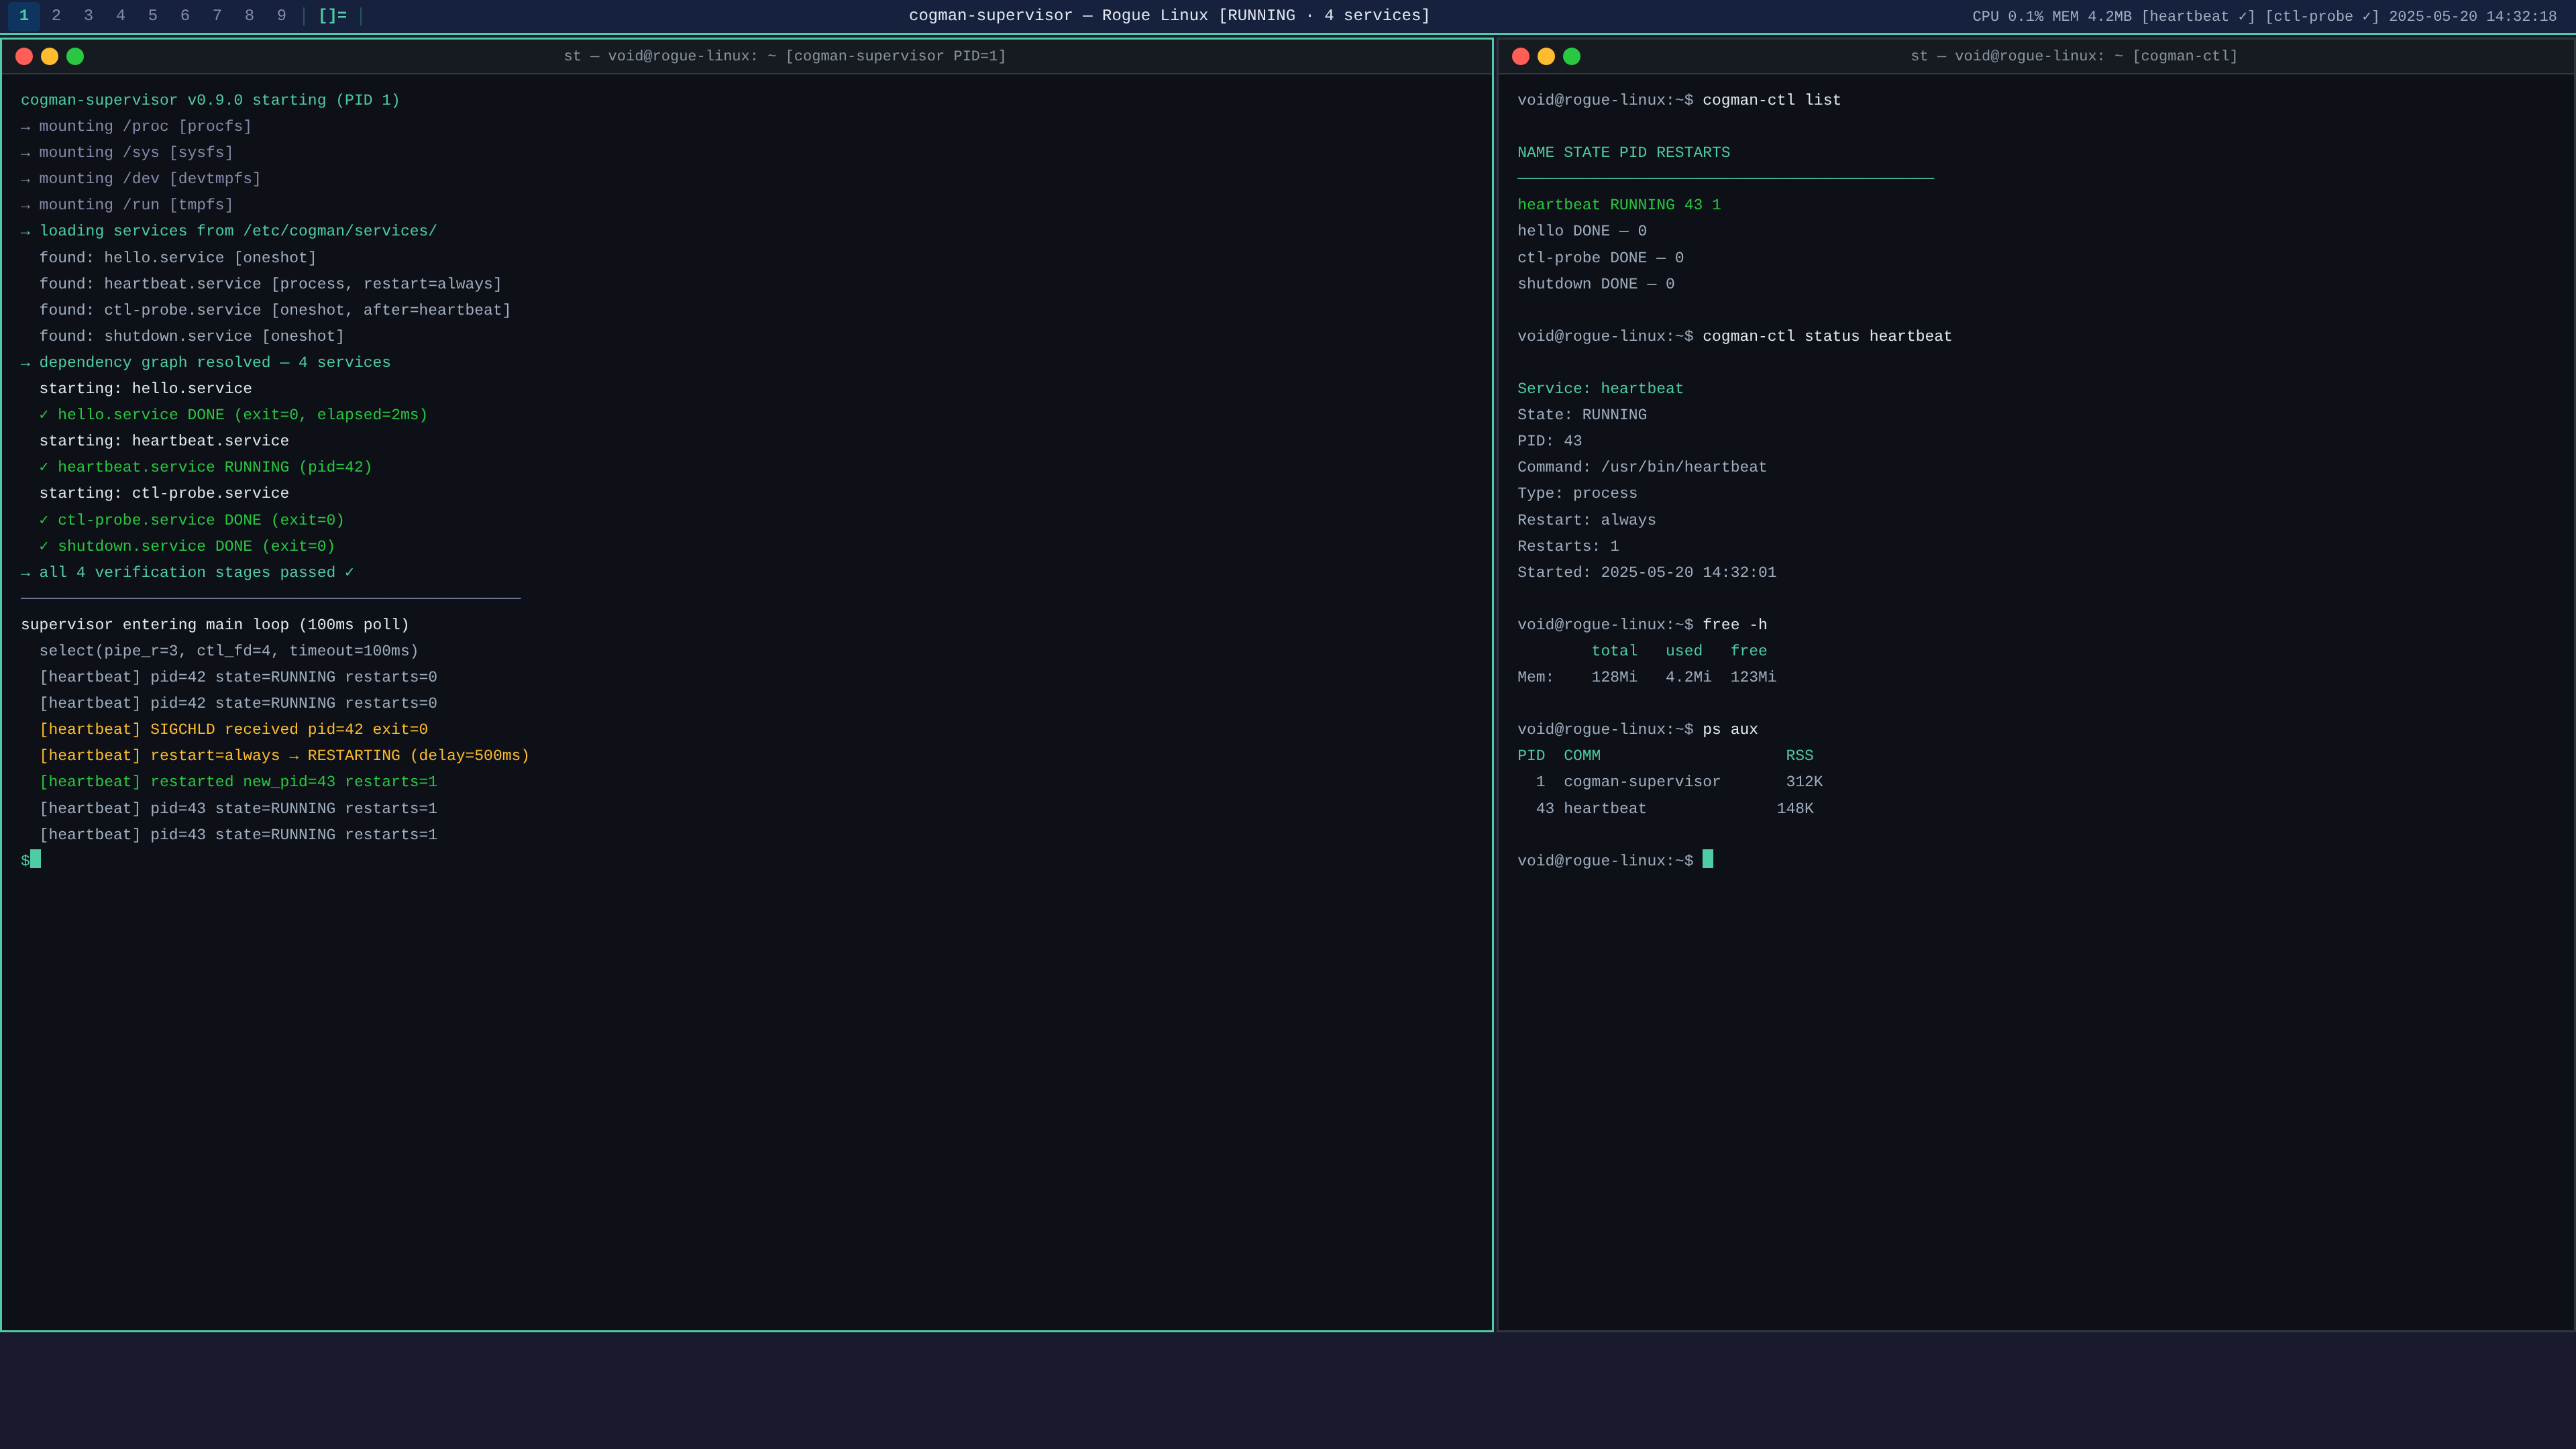
\includegraphics[width=0.92\textwidth]{extra_dwm_ui.png}
  \caption{DWM Window Manager running on Rogue Linux under QEMU with X11}
  \label{fig:dwm}
\end{figure}

\begin{figure}[H]
  \centering
  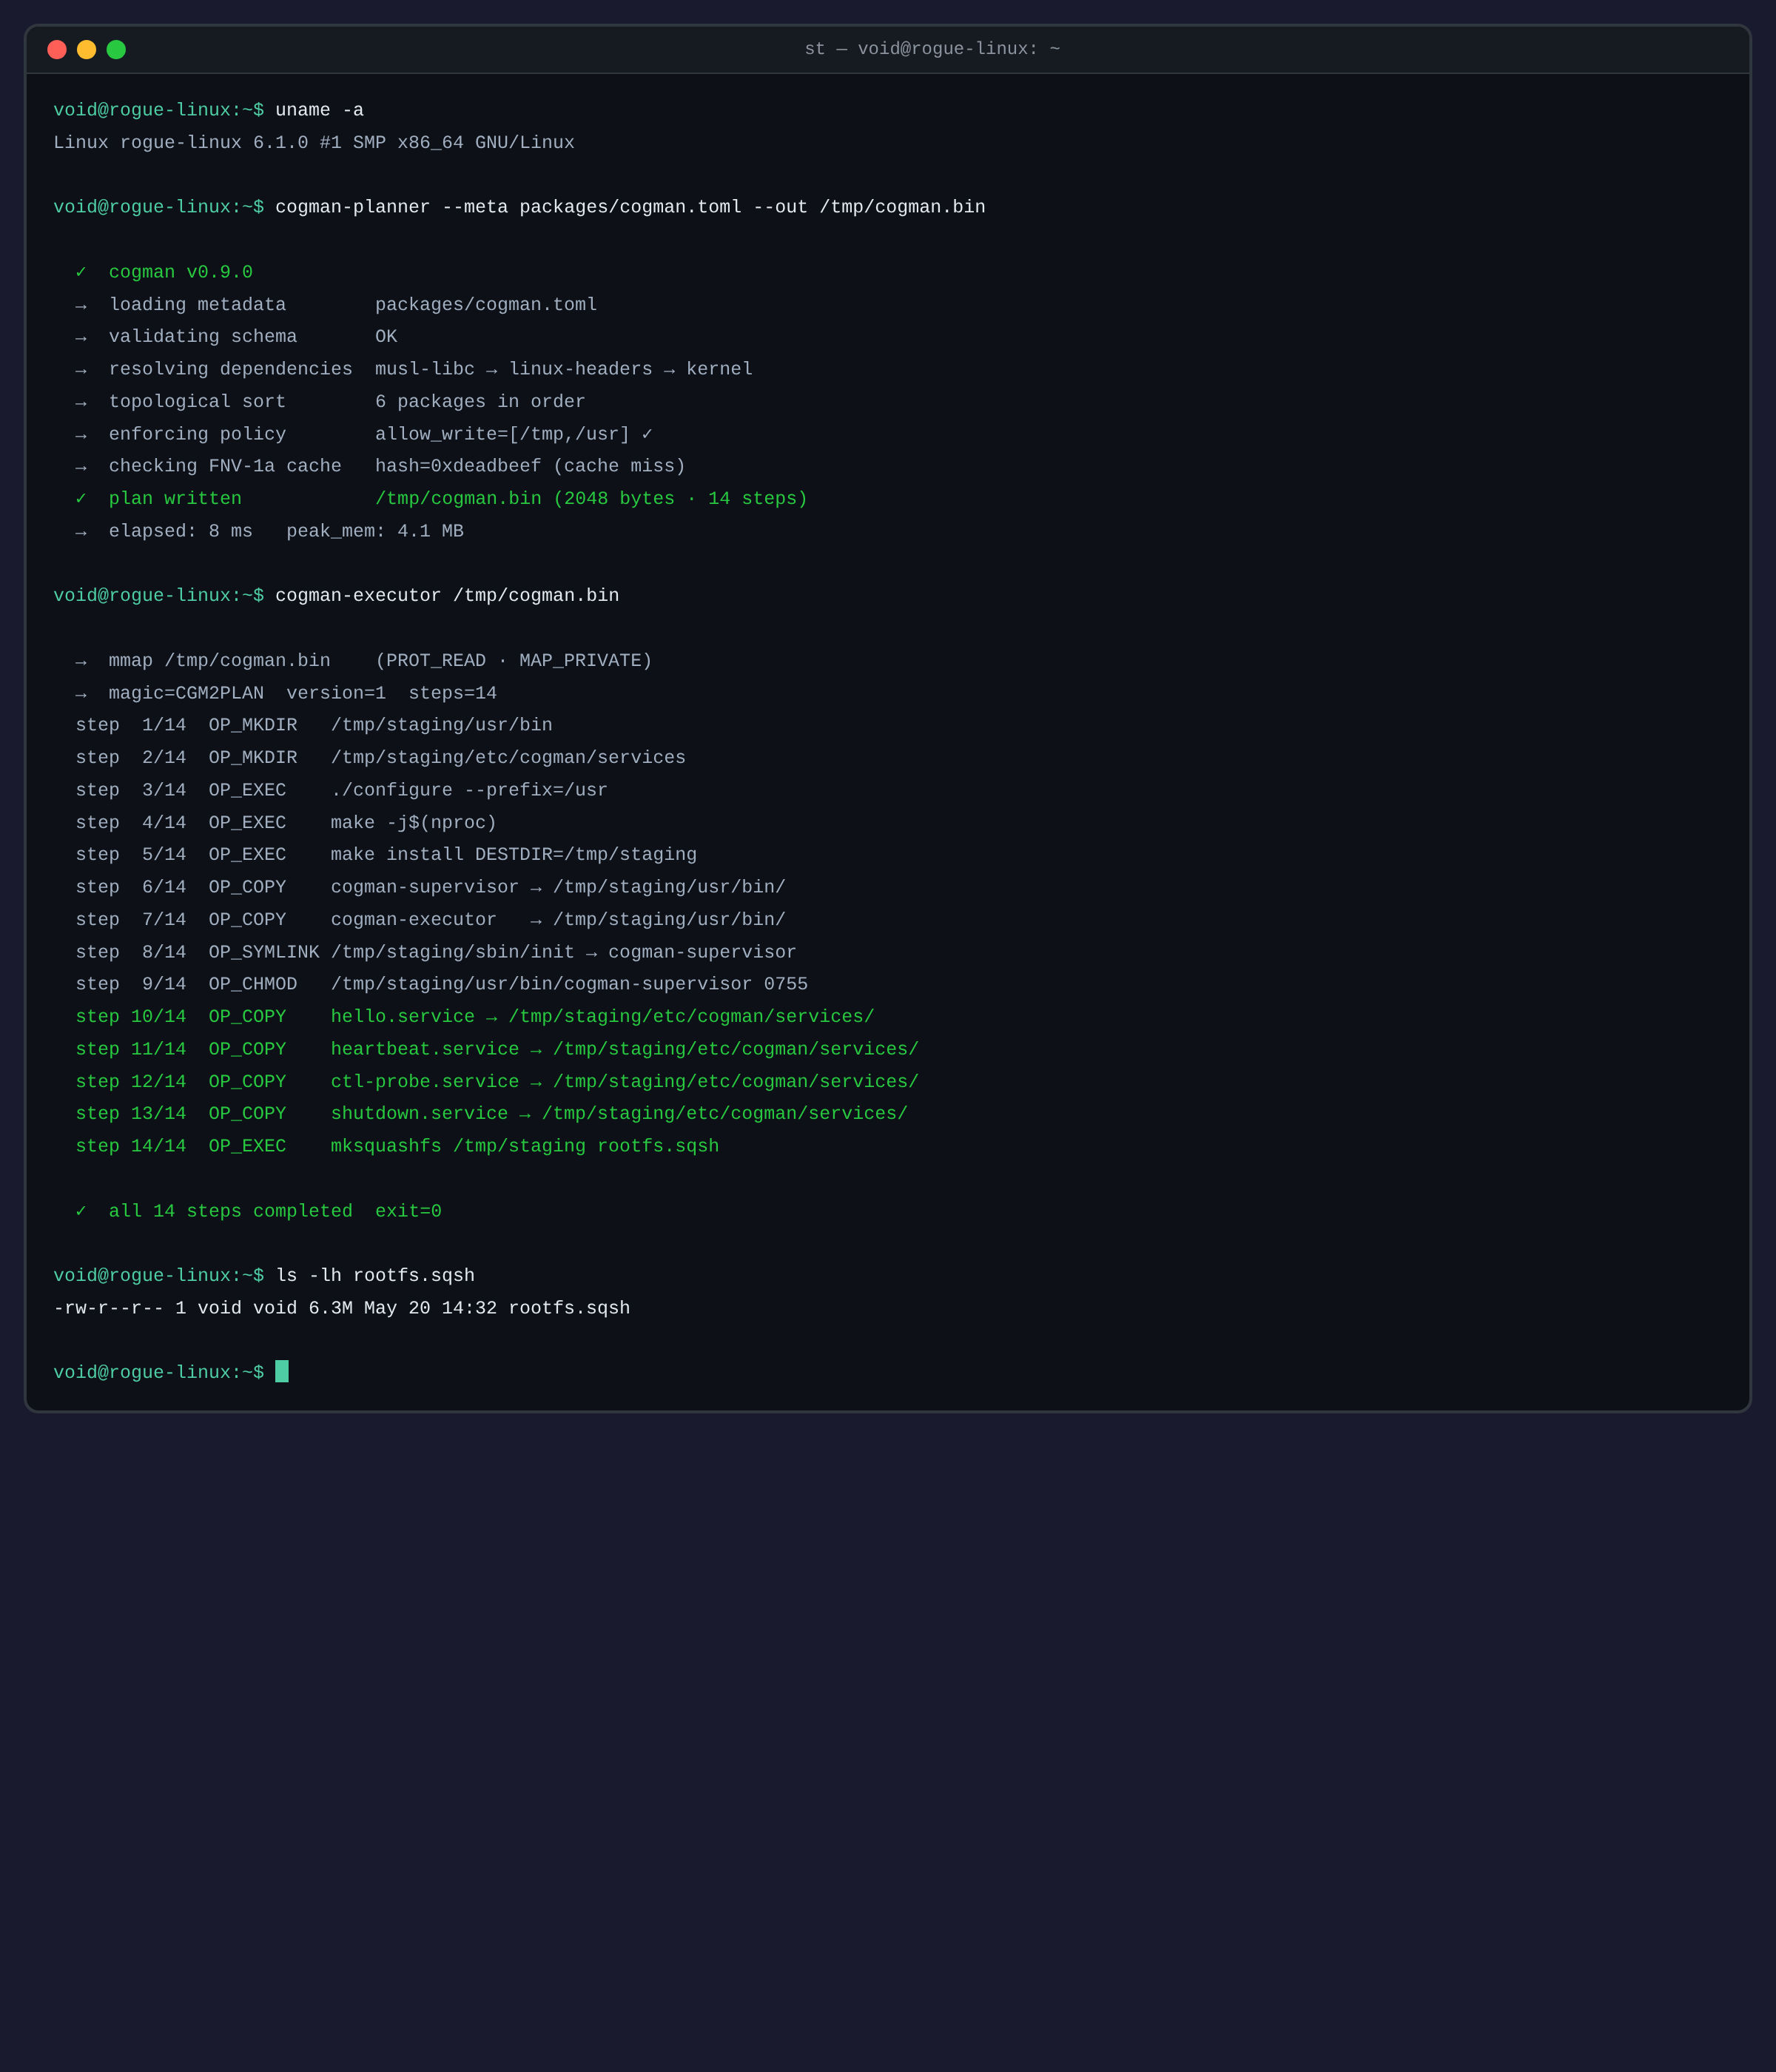
\includegraphics[width=0.92\textwidth]{extra_terminal.png}
  \caption{Terminal Environment --- cogman-ctl commands and BusyBox shell session}
  \label{fig:terminal}
\end{figure}

%% ══════════════════════════════════════ APPENDIX C — INTERNSHIP CERTIFICATES
\clearpage
\phantomsection
\addcontentsline{toc}{chapter}{Appendix C: Internship Certificates}
\begin{center}
{\large\bfseries APPENDIX C}\\[4pt]
{\large\bfseries\MakeUppercase{Internship Certificates}}
\end{center}
\vspace{4pt}

\begin{figure}[H]
  \centering
  \includegraphics[width=\textwidth,height=0.82\textheight,keepaspectratio]%
    {../intership/Sridharan.png}
  \caption*{Internship Certificate --- Sridharan T (620822205302)}
\end{figure}
\clearpage

\begin{figure}[H]
  \centering
  \includegraphics[width=\textwidth,height=0.92\textheight,keepaspectratio]%
    {../intership/ShanmugaSrilan.png}
  \caption*{Internship Certificate --- Praveenraj G (620822205078)}
\end{figure}
\clearpage

\begin{figure}[H]
  \centering
  \includegraphics[width=\textwidth,height=0.92\textheight,keepaspectratio]%
    {../intership/Praveenraj.png}
  \caption*{Internship Certificate --- Shanmuga Srilan T (620822205097)}
\end{figure}
\clearpage

\begin{figure}[H]
  \centering
  \includegraphics[width=\textwidth,height=0.92\textheight,keepaspectratio]%
    {../intership/Mugilan.png}
  \caption*{Internship Certificate --- Mugilan K (620822205063)}
\end{figure}

% ══════════════════════════════════════════════════════ REFERENCES
\clearpage
\addcontentsline{toc}{chapter}{References}
\begin{thebibliography}{20}

\bibitem{buildroot}
Buildroot Project.
\textit{Buildroot: Making Embedded Linux Easy}.
2023. \url{https://buildroot.org/}

\bibitem{yocto}
Yocto Project.
\textit{Yocto Project Documentation}.
2023. \url{https://docs.yoctoproject.org/}

\bibitem{nix}
E. Dolstra.
\textit{The Purely Functional Software Deployment Model}.
PhD Thesis, Utrecht University, 2006.

\bibitem{systemd}
L. Poettering et al.
\textit{systemd -- System and Service Manager}.
2010--present. \url{https://systemd.io/}

\bibitem{daemontools}
D. J. Bernstein.
\textit{daemontools: Service Management}.
2000. \url{https://cr.yp.to/daemontools.html}

\bibitem{s6}
L. Bercot.
\textit{s6 -- A Small Supervision Suite}.
2012--present. \url{https://skarnet.org/software/s6/}

\bibitem{rust}
The Rust Foundation.
\textit{The Rust Programming Language}, 2nd ed.
2024. \url{https://doc.rust-lang.org/book/}

\bibitem{serde}
Serde Working Group.
\textit{serde -- A Serialisation Framework for Rust}.
2024. \url{https://serde.rs/}

\bibitem{qemu}
QEMU Project.
\textit{QEMU -- The Fast! Processor Emulator}.
2024. \url{https://www.qemu.org/}

\bibitem{qwen}
Alibaba Cloud.
\textit{Qwen2.5 Technical Report}.
arXiv:2412.15115, 2024.

\bibitem{llamacpp}
G. Gerganov et al.
\textit{llama.cpp: LLM Inference in C/C++}.
2022. \url{https://github.com/ggerganov/llama.cpp}

\bibitem{c11}
ISO/IEC.
\textit{ISO/IEC 9899:2011 -- Programming Languages: C}.
International Standard, 2011.

\bibitem{kerrisk}
M. Kerrisk.
\textit{The Linux Programming Interface}.
No Starch Press, San Francisco, 2010.

\bibitem{stevens}
W. R. Stevens and S. A. Rago.
\textit{Advanced Programming in the UNIX Environment}, 3rd ed.
Addison-Wesley, 2013.

\bibitem{repro}
Reproducible Builds Project.
\textit{Reproducible Builds}.
2024. \url{https://reproducible-builds.org/}

\bibitem{busybox}
BusyBox Project.
\textit{BusyBox: The Swiss Army Knife of Embedded Linux}.
2023. \url{https://busybox.net/}

\bibitem{bazel}
Bazel Authors.
\textit{Bazel Documentation: Remote Caching}.
2024. \url{https://bazel.build/remote/caching}

\bibitem{posix}
The Open Group.
\textit{POSIX.1-2017 -- Base Specifications Issue 7}.
2017. \url{https://pubs.opengroup.org/}

\bibitem{toml}
T. Preston-Werner.
\textit{TOML v1.0.0 Specification}.
2021. \url{https://toml.io/en/v1.0.0}

\bibitem{linux}
L. Torvalds et al.
\textit{Linux Kernel Source}.
2024. \url{https://kernel.org/}

\end{thebibliography}

%% ══════════════════════════════════════ PROGRAM OUTCOMES & COURSE OUTCOMES
\clearpage
\phantomsection
\addcontentsline{toc}{chapter}{Program Outcomes and Course Outcomes}
\enlargethispage{6\baselineskip}

\begin{center}
  {\large\bfseries PROGRAM OUTCOMES (POs)}
\end{center}
\vspace{4pt}

{\fontsize{9.5}{12.5}\selectfont
\renewcommand{\arraystretch}{1.08}
\setlength{\tabcolsep}{5pt}
\noindent\begin{tabular}{|p{0.09\textwidth}|p{0.215\textwidth}|p{0.615\textwidth}|}
\hline
\textbf{PO 1}  & \textbf{Engineering knowledge}         & Apply the knowledge of mathematics, science, engineering fundamentals and an engineering specialization to the solution of complex engineering problems. \\
\hline
\textbf{PO 2}  & \textbf{Problem analysis}               & Identify, formulate, review research literature, and analyze complex engineering problems reaching substantiated conclusions using first principles of mathematics, natural sciences, and engineering sciences. \\
\hline
\textbf{PO 3}  & \textbf{Design/development of solutions}& Design solutions for complex engineering problems and design system components or processes that meet the specified needs with appropriate consideration for the public health and safety, and the cultural, societal, and environmental considerations. \\
\hline
\textbf{PO 4}  & \textbf{Conduct investigations of complex problems} & Use research-based knowledge and research methods including design of experiments, analysis and interpretation of data, and synthesis of the information to provide valid conclusions. \\
\hline
\textbf{PO 5}  & \textbf{Modern tool usage}              & Create, select, and apply appropriate techniques, resources, and modern engineering and IT tools including prediction and modeling to complex engineering activities with an understanding of the limitations. \\
\hline
\textbf{PO 6}  & \textbf{The engineer and society}       & Apply reasoning informed by the contextual knowledge to assess societal, health, safety, legal and cultural issues and the consequent responsibilities relevant to the professional engineering practice. \\
\hline
\textbf{PO 7}  & \textbf{Environment and sustainability} & Understand the impact of the professional engineering solutions in societal and environmental contexts, and demonstrate the knowledge of, and need for sustainable development. \\
\hline
\textbf{PO 8}  & \textbf{Ethics}                         & Apply ethical principles and commit to professional ethics and responsibilities and norms of the engineering practice. \\
\hline
\textbf{PO 9}  & \textbf{Individual and team work}       & Function effectively as an individual, and as a member or leader in diverse teams, and in multidisciplinary settings. \\
\hline
\textbf{PO 10} & \textbf{Communication}                  & Communicate effectively on complex engineering activities with the engineering community and with society at large, such as, being able to comprehend and write effective reports and design documentation, make effective presentations, and give and receive clear instructions. \\
\hline
\textbf{PO 11} & \textbf{Project management and finance} & Demonstrate knowledge and understanding of the engineering and management principles and apply these to one's own work, as a member and leader in a team, to manage projects and in multidisciplinary environments. \\
\hline
\textbf{PO 12} & \textbf{Life-long learning}             & Recognize the need for, and have the preparation and ability to engage in independent and life-long learning in the broadest context of technological change. \\
\hline
\end{tabular}
}

%% ─────────────────────────── COURSE OUTCOMES PAGE ───────────────────────────
\clearpage
\phantomsection
\vspace*{\fill}

\begin{flushleft}
{\fontsize{11}{14}\selectfont
\begin{tabular}{@{}ll@{}}
\textbf{COURSE CODE \& NAME} & :\quad C412 -- (CS3811 -- PROJECT) \\[2pt]
\textbf{REGULATION}          & :\quad R2021 \\[2pt]
\textbf{YEAR / SEM}          & :\quad IV / VIII \\
\end{tabular}
}
\end{flushleft}
\vspace{14pt}

\begin{center}
  {\large\bfseries COURSE OUTCOMES}
\end{center}
\vspace{6pt}

{\fontsize{11}{14}\selectfont
\renewcommand{\arraystretch}{1.3}
\noindent\begin{tabular}{@{}p{0.10\textwidth}p{0.04\textwidth}p{0.81\textwidth}@{}}
\textbf{C412.1} & E & Analyze the problem requirements for designing a minimal Linux distribution targeting cybersecurity and penetration-testing operations. \\[3pt]
\textbf{C412.2} & C & Develop the Cogman toolchain modules --- planner, executor, and supervisor --- integrating build-time and runtime management without external dependencies. \\[3pt]
\textbf{C412.3} & E & Choose and configure appropriate kernel options, security tools (nmap, tcpdump, socat), and system services for a hardened minimal rootfs. \\[3pt]
\textbf{C412.4} & C & Combine all components through a unified pipeline, verify correctness via automated QEMU boot tests, and validate the complete system against all test cases. \\[3pt]
\textbf{C412.5} & C & Elaborate performance benchmarks, document the complete system design, and compile the final project report and presentation. \\
\end{tabular}
}

\vspace{20pt}

\begin{center}
{\fontsize{11}{14}\selectfont
\renewcommand{\arraystretch}{1.3}
\setlength{\tabcolsep}{3pt}
\begin{adjustbox}{max width=\linewidth}
\begin{tabular}{|l|c|c|c|c|c|c|c|c|c|c|c|c|c|c|}
\hline
\textbf{CO/PO} & \textbf{PO1} & \textbf{PO2} & \textbf{PO3} & \textbf{PO4} & \textbf{PO5} & \textbf{PO6} & \textbf{PO7} & \textbf{PO8} & \textbf{PO9} & \textbf{PO10} & \textbf{PO11} & \textbf{PO12} & \textbf{PSO1} & \textbf{PSO2} \\
\hline
C412.1 & 3 & 3 & 2 & 2 & 2 & 1 & -- & 2 & 2 & 2 & 2 & 3 & 3 & 3 \\
\hline
C412.2 & 3 & 3 & 3 & 2 & 3 & 2 & -- & 3 & 3 & 2 & 2 & 3 & 3 & 3 \\
\hline
C412.3 & 3 & 3 & 3 & 3 & 3 & 2 & 2 & 3 & 3 & 3 & 2 & 3 & 2 & 3 \\
\hline
C412.4 & 3 & 3 & 3 & 3 & 3 & 2 & 3 & 3 & 3 & 3 & 3 & 3 & 3 & 3 \\
\hline
C412.5 & 3 & 3 & 3 & 3 & 3 & 2 & 3 & 3 & 3 & 3 & 3 & 3 & 3 & 3 \\
\hline
\textbf{C412} & \textbf{3.00} & \textbf{3.00} & \textbf{2.80} & \textbf{2.60} & \textbf{2.80} & \textbf{1.80} & \textbf{2.67} & \textbf{2.80} & \textbf{2.80} & \textbf{2.60} & \textbf{2.40} & \textbf{3.00} & \textbf{2.80} & \textbf{3.00} \\
\hline
\end{tabular}
\end{adjustbox}
}
\end{center}

\vspace*{\fill}

\end{document}
